%  Bow-Tie Architecture in the Drosophila melanogaster Connectome
%  Master thesis, University of Calabria.
%
%  Sorgente in un file unico. Si compila con pdfLaTeX; la bibliografia e'
%  in fondo, non serve un .bib separato.
%  Non restano campi da completare: frontespizio, anno accademico e
%  bibliografia sono tutti definitivi.

\documentclass[12pt,a4paper,oneside]{article}

%----------------------------------------------------------------------
%  pacchetti
%----------------------------------------------------------------------
\usepackage[utf8]{inputenc}
\usepackage[T1]{fontenc}
\usepackage[english]{babel}
\usepackage{lmodern}
\usepackage{microtype}

\usepackage[a4paper,top=3cm,bottom=3cm,left=3cm,right=3cm]{geometry}
\usepackage{setspace}
\onehalfspacing

\usepackage{amsmath,amssymb,amsthm}
\usepackage{booktabs}
\usepackage{multirow}
\usepackage{graphicx}
\graphicspath{{figures/}}
\usepackage{float}
\usepackage{caption}
\usepackage{subcaption}

\usepackage{xcolor}
\usepackage[hidelinks]{hyperref}
\usepackage{url}
\usepackage{tikz}
\usetikzlibrary{arrows.meta,positioning,fit,backgrounds}

% figure e tabelle numerate progressivamente
\usepackage{chngcntr}
\counterwithout{figure}{section}
\counterwithout{table}{section}
\counterwithout{equation}{section}

\usepackage{fancyhdr}
\pagestyle{fancy}
\fancyhf{}
\fancyhead[L]{\small\MakeUppercase{\leftmark}}
% logo istituzionale in alto a destra:
% \fancyhead[R]{\includegraphics[height=1.0cm]{unical_logo.png}}
\fancyfoot[C]{\thepage}
\renewcommand{\headrulewidth}{0.4pt}
\renewcommand{\sectionmark}[1]{\markboth{\thesection\quad #1}{}}

% ambienti per definizioni e proposizioni
\theoremstyle{definition}
\newtheorem{definition}{Definition}[section]
\theoremstyle{plain}
\newtheorem{proposition}{Proposition}[section]
\newtheorem{lemma}{Lemma}[section]

% abbreviazioni usate nel testo
\newcommand{\Drosophila}{\textit{Drosophila melanogaster}}
\newcommand{\Dros}{\textit{Drosophila}}
\newcommand{\kin}{k_{\mathrm{in}}}
\newcommand{\kout}{k_{\mathrm{out}}}
\newcommand{\sigmapi}{\ensuremath{\Sigma\Pi}}
\newcommand{\neff}{n^{\mathrm{eff}}_{\mathrm{waist}}}
\newcommand{\code}[1]{\texttt{#1}}

%=======================================================================
\begin{document}

%----------------------------------------------------------------------
%  frontespizio
%----------------------------------------------------------------------
\begin{titlepage}
\centering
\vspace*{1.5cm}

% il logo e' quadrato: dato in larghezza sarebbe alto quasi 7 cm
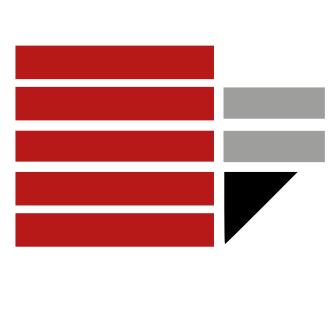
\includegraphics[height=3cm]{logo.png}\\[1.2cm]

{\scshape\Large University of Calabria\par}
\vspace{0.4cm}
{\scshape Department of Mathematics and Computer Science\par}
\vspace{0.3cm}
{\scshape Master's Course in \textsc{Computer Science and Artificial Intelligence}\par}

\vspace{2.2cm}

{\huge\bfseries Bow-Tie Architecture in the\\[0.3cm]
\Drosophila{} Connectome:\\[0.3cm]
A Two-Scale Structural Analysis\par}

\vspace{2.8cm}

\begin{minipage}[t]{0.45\textwidth}
\raggedright
\large
Supervisor:\\[0.3cm]
\textbf{Professor Giorgio Terracina}
\end{minipage}
\hfill
\begin{minipage}[t]{0.45\textwidth}
\raggedleft
\large
Candidate:\\[0.3cm]
\textbf{Federico Di Franco}\\
\textbf{Student ID: 263678}
\end{minipage}

\vfill
{\scshape Academic Year 2025/2026\par}
\end{titlepage}

\clearpage
\pagenumbering{roman}

%----------------------------------------------------------------------
%  dichiarazione
%----------------------------------------------------------------------
\section*{Declaration}
\markboth{DECLARATION}{DECLARATION}
\thispagestyle{plain}

I hereby declare and confirm that this thesis is entirely the result of my
own original work. Where other sources of information have been used, they
have been indicated as such and properly acknowledged. I further declare
that this or similar work has not been submitted for credit elsewhere.

This printed thesis is identical with the electronic version submitted.

\vspace{2.5cm}

\noindent
\begin{minipage}[t]{0.45\textwidth}
\raggedright
Date\\[1.4cm]
\rule{5cm}{0.4pt}
\end{minipage}
\hfill
\begin{minipage}[t]{0.45\textwidth}
\raggedleft
Signature\\[1.4cm]
\rule{5cm}{0.4pt}
\end{minipage}

\clearpage

%----------------------------------------------------------------------
%  abstract
%----------------------------------------------------------------------
\section*{Abstract}
\addcontentsline{toc}{section}{Abstract}
\markboth{ABSTRACT}{ABSTRACT}
% due righe in piu' su questa pagina: senza, l'abstract sborda e quelle due
% righe si prendono da sole la pagina successiva
\enlargethispage{2\baselineskip}

Understanding how cognitive functions emerge from the physical wiring of the
brain is one of the central challenges of modern neuroscience. The recent
release of the synapse-resolution connectome of the adult \Drosophila{}
brain has made it possible, for the first time, to address this question
computationally on a complete nervous system.

This thesis asks whether the \Dros{} connectome exhibits a bow-tie, or
hourglass, architecture: whether many input pathways converge onto a small
set of intermediate elements which then diverge again towards many outputs.
The question is addressed at two complementary scales that serve as a check
on each other. At the local scale we count, exhaustively and exactly, motifs
in which $\kin$ groups of neurons converge onto a single intermediate group,
called the waist, which in turn projects onto $\kout$ further groups. The
counting uses a flow-vector formulation that never enumerates the search
space, which is what makes an exhaustive treatment possible at all. At the
global scale we compute the $\tau$-core of the network, the smallest set of
neurons carrying a prescribed fraction of all sensory-to-motor paths, and
from it the hourglass score defined by Sabrin et al.

The thesis makes four contributions. The first is theoretical: we
characterise exactly when motif counts compose, showing that the boundary
between patterns countable with a linear flow vector and patterns requiring
a sum-of-products formulation is precisely the presence of branching, and
that cyclic patterns are not factorisable over vectors at all. The second is
computational: a search engine that makes exhaustive counting tractable at
connectome scale, gaining a factor of $219$ on the worst bottleneck through
a sparse reformulation, and verified row by row against an independent
reference implementation. The third is empirical: an analysis of all four
level windows of the hierarchy rather than a single one, which reveals that
the architecture changes qualitatively with depth, with signatures involving
a purely lateral branch growing from $38.0\%$ to $82.6\%$ of all motif
instances.
The fourth is methodological: a hypothesis carried through to the point
where it can be tested rather than asserted. An apparent neurochemical
difference between backward and forward waists is significant on the shallow
window, is traced there to regional composition, and does not replicate
across the remaining windows; it is therefore reported as an open question
about the optic lobe rather than as a property of the connectome, together
with the procedure that established the distinction.

The hourglass effect is present but depends on how paths are routed, with a
score of $0.498$ under structural routing against values between $0.74$ and
$0.87$ reported for \textit{C.\ elegans}. The two scales agree on the
mid-hierarchy waists of the olfactory pathway and disagree on input groups,
and that disagreement turns out to be interpretable rather than
contradictory.

\clearpage

%----------------------------------------------------------------------
%  indici
%----------------------------------------------------------------------
\tableofcontents
\clearpage
\listoffigures
\clearpage
\listoftables
\clearpage

\section*{Glossary}
\addcontentsline{toc}{section}{Glossary}
\markboth{GLOSSARY}{GLOSSARY}

\begin{tabbing}
\hspace{2.5cm}\= \kill
\textbf{AL}      \> Antennal Lobe, the first olfactory processing centre \\
\textbf{BLAS}    \> Basic Linear Algebra Subprograms \\
\textbf{BWD}     \> Backward, an edge running from a deeper to a shallower level \\
\textbf{E/I}     \> Excitatory / Inhibitory \\
\textbf{EB}      \> Ellipsoid Body \\
\textbf{EM}      \> Electron Microscopy \\
\textbf{FB}      \> Fan-shaped Body, a neuropil of the central complex \\
\textbf{FDR}     \> False Discovery Rate \\
\textbf{FWD}     \> Forward, an edge running from a shallower to a deeper level \\
\textbf{GNG}     \> Gnathal Ganglia \\
\textbf{LAT}     \> Lateral, an edge between neurons of the same level \\
\textbf{LH}      \> Lateral Horn \\
\textbf{LO}      \> Lobula, a visual processing neuropil \\
\textbf{LOP}     \> Lobula Plate \\
\textbf{MB}      \> Mushroom Body, the centre for olfactory learning \\
\textbf{MB\_CA}  \> Mushroom Body Calyx, its input region \\
\textbf{ME}      \> Medulla, the largest visual neuropil \\
\textbf{PLP}     \> Posterior Lateral Protocerebrum \\
\textbf{PRW}     \> Prow \\
\textbf{PVLP}    \> Posterior Ventrolateral Protocerebrum \\
\textbf{\sigmapi{}} \> The sum-of-products formulation used for branching patterns \\
\end{tabbing}

\clearpage
\pagenumbering{arabic}

%=======================================================================
\section{Introduction}
\label{sec:introduction}
%=======================================================================

\subsection{Motivation}
\label{sec:motivation}

One of the most ambitious goals of modern neuroscience is to understand how
cognitive functions such as memory, learning and decision-making emerge from
the physical structure of the brain \cite{bassett2017}. For most of the
history of the field this question could only be approached indirectly.
Lesion studies, electrophysiology and imaging observed neural activity
without access to the underlying wiring diagram, which meant that structural
hypotheses about brain function could be formulated but not rigorously
tested.

Advances in large-scale electron microscopy and automated image segmentation
have begun to dissolve this barrier. Connectomics, the science of producing
complete maps of synaptic connectivity in neural tissue \cite{bullmore2009},
now yields global wiring diagrams in which every neuron and every synapse is
labelled. Where traditional neural sampling reconstructed a few hundred
neurons at a time, a connectome provides the entire network at once, which
permits computational analyses at a scale and resolution that were
previously out of reach. The adult \Drosophila{} brain has emerged as the
premier model organism for this pursuit: it contains only about
$140{,}000$ neurons, some five orders of magnitude fewer than the human
brain, and yet supports a behavioural repertoire spanning visual pursuit,
olfactory learning, sleep regulation and courtship \cite{lin2024}.

The availability of a complete directed graph of a complex brain creates an
opportunity, but it does not by itself create understanding. A raw
connectome is a sparse, cyclic and heterogeneous directed graph with no
intrinsic coordinate system. Artificial neural networks are designed with
layered topologies through which information flows in one direction;
biological circuits are not. They feature extensive recurrent connectivity,
and feedback projections from deeper processing stages back to earlier ones
are plentiful relative to feed-forward ones \cite{winding2023}. This makes
it structurally difficult to say what ``earlier'' and ``later'' mean in a
circuit, and consequently difficult to compare connectivity patterns across
brain regions in any principled way, because there is no agreed axis along
which to place them.

A central concept for making sense of this complexity is that of network
motifs: small recurring connectivity patterns that occur in a network far
more often than chance would predict \cite{milo2002}. At the level of neural
circuits, motifs are the elementary computational building blocks from which
larger structures are assembled. A feed-forward chain of three neurons
implements a simple relay; adding a feedback arc to that chain turns it into
a loop capable of sustaining activity over time; a lateral connection
between two populations firing in parallel creates a cross-stream
interaction. If one knows which motifs are common in a given connectome, and
how their composition changes from one brain region to another, it becomes
possible to read circuit-level computational strategies off the wiring
diagram alone.

This thesis focuses on one particular architectural template, the bow-tie,
also called the hourglass. A bow-tie is a structure in which many inputs
converge onto a narrow set of intermediate elements, called the waist, which
then diverge again towards many outputs. The template is known to recur
across widely different complex systems: cellular metabolism, the Internet
protocol stack and manufacturing supply networks all display it
\cite{sabrin2020}. Its presence is informative because it implies that the
system compresses information through a narrow channel before redistributing
it, and that in turn constrains both what the system can compute and how
vulnerable it is to the loss of individual components. If the \Dros{} brain
is organised this way, the neurons occupying the waist are the ones through
which most of the sensory-to-motor traffic must pass, which makes them
natural targets for functional investigation.

\subsection{Problem Statement}
\label{sec:problem}

The technical question of this thesis can be stated as follows. Given the
full synaptic graph of the adult \Dros{} brain, comprising $134{,}181$
neurons with an assigned hierarchical level and $2{,}700{,}513$ synaptic
pairs, determine whether the network exhibits a bow-tie architecture, at
what scale it does so, and which anatomical structures occupy the waist. The
problem decomposes into three sub-problems, each of which has to be solved
before the next becomes meaningful.

The first is that of counting without enumeration. A bow-tie motif with two
input groups and two output groups, searched over the groups of a single
level window, induces a space of more than eight billion candidate
combinations. Explicit enumeration of subgraph occurrences, in the style of
the classical subgraph isomorphism algorithms \cite{ullmann1976,cordella2004},
is entirely infeasible at that scale. What is required instead is a counting
formulation that produces exact occurrence counts without ever materialising
an individual match. Such formulations do exist, but they do not exist for
every pattern, and the conditions under which they apply have to be
established rather than assumed. The condition turns out to be a property of
the shape of the pattern and nothing else: a count factorises when the
pattern contains no cycle, and does not when it contains one.

The second sub-problem concerns the relationship between two different ways
of asking the same question. Motif counting is inherently local: it measures
convergence and divergence in the immediate neighbourhood of a group of
neurons. The hourglass effect, by contrast, is a global property of
end-to-end information flow through the whole network. These are two
different measurements of the same architectural intuition, and there is no
guarantee that they agree. Establishing whether they do, and characterising
precisely where they do not, is part of the problem rather than an
afterthought, because a disagreement between two independent measurements is
either a warning that one of them is wrong or a finding in its own right.

The third sub-problem is that of distinguishing structure from composition.
Anatomical regions of the fly brain differ systematically in size, in
connection density and in neurotransmitter composition. Any apparent
difference between two classes of motifs may therefore reflect merely
\emph{where} those motifs happen to live rather than \emph{what} they are.
Controlling for regional composition is essential, and so is repeating the
controlled comparison on data that did not suggest the hypothesis in the
first place. This thesis contains a case in which a controlled effect held
on one subset of the data, reversed on another and disappeared on the whole,
which is a pattern that looks convincingly significant at every stage until
the last one.

\subsection{Research Objectives}
\label{sec:objectives}

The first objective is to establish the algebra of pattern counting, by
determining which connectivity patterns admit a linear counting formulation,
which require a sum-of-products formulation, and which require quadratic
memory. The result should be a statement about the shape of the pattern
rather than an empirical rule of thumb, and it should be verifiable by
exhaustive enumeration on small graphs so that its correctness does not rest
on the derivation alone.

The second objective is to make exhaustive counting tractable, by designing
and implementing a search engine capable of counting all bow-tie motifs over
the full connectome, for every level window, in hours rather than days. Here
correctness must be verified against an independent reference
implementation, not merely inferred from the mathematics, because an
optimisation that is correct in principle can still be wrong in code.

The third objective is to characterise the architecture at both scales, by
applying the local motif search and the global hourglass analysis to the
same connectome, reporting where the two converge and where they diverge,
and interpreting the divergence rather than explaining it away.

The fourth objective is to test structural hypotheses with adequate
controls. This means evaluating the statistical significance of the observed
motifs against several complementary null models rather than one, and
testing biological hypotheses about the waists, in particular whether
backward and forward waists differ in neurotransmitter composition,
with explicit controls for regional composition and with replication across
independent level windows.

\subsection{Contributions}
\label{sec:contributions}

The theoretical contribution of this thesis is an exact characterisation of
when motif counts compose, developed in Section~\ref{sec:pattern-algebra}.
Counting occurrences of a pattern means counting the ways it can be laid
over the graph, that is, the ways of assigning a neuron to each node of the
pattern so that every edge of the pattern lands on an edge of the graph;
these assignments are called \emph{homomorphisms}. Both the cost of counting
them and the way counts combine depend only on the shape of the pattern. Paths admit a pure matrix
product and their counts add across unions of node groups; trees require an
element-wise product at every branching node and their counts do not add;
cyclic patterns cannot be factorised over vectors at all. The boundary
between the tractable and the intractable is therefore exactly the presence
of branching, and an exhaustive catalogue up to four nodes shows that
$87\%$ of connected patterns already fall on the intractable side.

The computational contribution is a search engine that is both fast and
verified, described in Section~\ref{sec:engine}. Reformulating the inner
loop as a single matrix product delegated to optimised linear algebra
routines, and then switching to a sparse product for the largest waists,
yields a factor of $219$ on the worst bottleneck of the search. The engine
is verified row by row, across all $1{,}043{,}872$ rows and all $26$
columns, against a slow but readable reference implementation retained
specifically for that purpose.

The empirical contribution is an analysis across all four level windows of
the hierarchy, presented in Section~\ref{sec:results-windows}. Previous work
on this connectome has concentrated on a single window. Extending the
analysis to all four shows that the structure changes qualitatively with
depth: signatures involving a purely lateral branch account for $38.0\%$ of
all motif instances in the shallow window and $82.6\%$ in the deep one, and
the
deepest level of the hierarchy turns out to be the most internally dense
while remaining marginal as a waist.

The methodological contribution is a hypothesis pursued to the point where
the data can decide it, reported in Section~\ref{sec:results-nt}. The
hypothesis is that backward waists carry a distinct neurochemical signature,
and it is a natural one: inhibition is widely associated with feedback
control. It is significant on the shallow window, reverses sign on the
second and does not hold on the full connectome, and the reason is
identified: the two classes of motif sit in different brain regions, whose
neurochemistry differs. What survives is a narrower and better specified
claim about the medulla, stated as a hypothesis for future work, together
with the three-step procedure that separated it from the broader one. The
procedure is the transferable part, and it is described in enough detail to
be reused.

\subsection{Thesis Outline}
\label{sec:outline}

Section~\ref{sec:background} introduces the background required for the rest
of the work: the graph formalism, the \Dros{} connectome and its
hierarchical decomposition, network motifs, and the hourglass framework of
Sabrin et al. Section~\ref{sec:methods} develops the counting theory, both
analysis pipelines, the statistical validation scheme and the computational
optimisations that make the analysis feasible. Section~\ref{sec:results}
presents the results, and Section~\ref{sec:conclusions} summarises the
contributions, states the limitations and outlines directions for further
work.

%=======================================================================
\section{Theoretical Background}
\label{sec:background}

This chapter assembles the four things the rest of the thesis needs, in the
order in which they become necessary.

It begins with the graph formalism and the matrix representation of a
network, which is what turns questions about connectivity into arithmetic
that a computer can do at this scale. It then describes the connectome
itself: what FlyWire measured, how its neurons are ordered along a
sensory-to-motor axis, what the anatomical labels mean, and how neurons are
grouped so that the search space becomes finite. It introduces network
motifs, the notion that recurring small patterns are the building blocks of
a network, and the classification of those patterns by direction that this
thesis relies on. Finally it sets out the bow-tie and the hourglass, which
are the two objects the whole analysis is about, and explains why they are
not the same thing even though the literature often uses the words
interchangeably.

That last distinction organises everything that follows. A \emph{bow-tie} is
a local pattern: a few groups converging on one and then diverging again. An
\emph{hourglass} is a global property: the whole network routing its traffic
through a narrow set of intermediaries. A network can have many of the first
without being the second, which is why this thesis measures both and then
asks whether they agree.
%=======================================================================

\subsection{Fundamentals of Network Science}
\label{sec:network-science}


Two things are needed before the connectome can be discussed at all: a
language for describing networks, and a representation that makes
computation on them possible. This section provides both, and neither is
developed further than the rest of the thesis actually uses.

\subsubsection{Graph Formalism}

A connectome is modelled as a directed graph $G = (V, E)$, where $V$ is the
set of neurons and $E \subseteq V \times V$ the set of synaptic connections.
An edge $(u,v) \in E$ indicates that neuron $u$ forms at least one chemical
synapse onto neuron $v$; the direction of the edge is the direction in which
the signal travels. Edges may additionally carry a weight $w(u,v)$ equal to
the number of individual synaptic contacts between the two neurons, which in
this dataset ranges from the reporting threshold of five up to several
hundred.

Throughout this thesis we work with the unweighted, de-duplicated graph, so
that an ordered pair of neurons contributes at most one edge regardless of
how many synapses connect them. This choice is deliberate and worth
justifying, because it discards information. Motif counting asks whether a
connectivity \emph{pattern} exists between particular neurons, not how
strong that connection is. If multiplicities were retained, a motif count
would conflate the number of distinct circuits realising a pattern with the
strength of the individual connections within them, and a single very
strongly connected pair could dominate the count of a pattern that occurs
only once. Since the quantity of interest here is how many distinct circuits
implement a given architecture, the unweighted graph is the correct object.

\subsubsection{Matrix Representations}

A graph can equally well be written as a matrix, and doing so is what makes
the analysis in this thesis possible, so it is worth setting out both the
representation and the one identity that is used throughout.

The \emph{adjacency matrix} $A \in \{0,1\}^{|V| \times |V|}$ records the
edges in a table: the entry $A_{uv}$ is $1$ if the edge $(u,v)$ is present
and $0$ otherwise. Written out in full this table is unusable at connectome
scale. With $134{,}181$ neurons it has more than $18$ billion entries,
occupying over $18$\,GB at one byte each, while the graph actually contains
$2{,}700{,}513$ edges: fewer than one entry in six thousand is non-zero.
Storing only the non-zero entries, as the Compressed Sparse Row format does,
is therefore not an optimisation but a precondition for holding the data in
memory at all, and every matrix in this thesis is stored that way.

The reason the representation matters, beyond storage, is that it turns a
question about connectivity into a multiplication. Consider the product
$A^2$. Its entry $(A^2)_{uv}$ is $\sum_w A_{uw} A_{wv}$, and each term of
that sum is $1$ exactly when there is an edge from $u$ to $w$ and one from
$w$ to $v$, that is, when $w$ is an intermediate step on a two-edge route
from $u$ to $v$. The sum therefore counts those routes. The same argument
applied repeatedly gives the general form: the number of directed paths of
length $k$ from a set of neurons $S$ to a set of neurons $T$ is
\begin{equation}
  \label{eq:path-count}
  \mathbf{1}_S^{\top} A^k \, \mathbf{1}_T ,
\end{equation}
where $\mathbf{1}_S$ is the indicator vector of $S$, the vector with a $1$
in the position of every neuron in $S$ and $0$ elsewhere. Counting paths, an
apparently combinatorial task, has become a matrix expression.

The practical value of this lies in how the expression is evaluated. Forming
$A^k$ explicitly would be hopeless, since even $A^2$ is far denser than $A$
and $A^3$ denser still. But the expression never needs to be evaluated that
way: one starts from the vector $\mathbf{1}_S$ and multiplies it by $A$
repeatedly, obtaining after each multiplication a vector whose entry at
neuron $v$ is the number of paths of that length reaching $v$. Only one
vector of $|V|$ numbers is ever held, and each multiplication touches each
edge once, so the whole computation costs $O(k \cdot |E|)$ time and
$O(|V|)$ memory instead of the cube of the number of neurons. An entire
class of counting problems thereby becomes linear in the size of the
network, and this vector, propagated step by step, is what
Section~\ref{sec:counting} will call the \emph{flow vector}.

Two cautions belong here. The identity counts \emph{walks} rather than
paths, since a route that visits the same neuron twice is included, and in a
graph with cycles the distinction is not cosmetic: the number of walks grows
without bound as their permitted length increases. And the trick works
because a chain is a sequence with no branches, so it does not carry over
unchanged to patterns that branch, which is the problem
Chapter~\ref{sec:methods} takes up.

\subsection{The \Drosophila{} Connectome}
\label{sec:connectome}


This section describes the object of study. It covers why the fruit fly is
the organism for which this analysis is possible at all, what the FlyWire
dataset contains, how its neurons are ordered along an axis running from
sensory input to motor output, what the anatomical labels mean, and how
neurons are grouped so that an exhaustive search becomes finite. The last two
are the choices on which every later result depends, and they are argued for
rather than assumed.

\subsubsection{A Model Organism for Structural Analysis}

The adult \Dros{} brain occupies a favourable position in the space of model
organisms. It is small enough to have been reconstructed completely at
synaptic resolution, which no vertebrate brain has been, and yet complex
enough to support behaviour that is not trivially reflexive. With
approximately $140{,}000$ neurons it retains sensory integration,
associative learning and memory, so that structural findings about it are
plausibly informative about principles that generalise, rather than being
peculiarities of a simple nervous system.

\subsubsection{The FlyWire Dataset}
\label{sec:dataset}

The data used in this work derive from the FlyWire reconstruction of the
adult female brain \cite{lin2024}, distributed through the Codex portal.
Four tables are used. The first lists synaptic pairs with their contact
counts, already filtered at a threshold of five synapses in the public
export, which removes the least reliable segmentation artefacts. The second
gives neuron identifiers together with their anatomical group assignment and
their predicted neurotransmitter, discussed below. The third provides
functional \emph{super-class} labels, which sort neurons by the role they
play rather than by where they sit: sensory, optic, central, descending and
five others, set out in full in Section~\ref{sec:groups}. The fourth
supplies the hierarchical level assignment described below.

The tables cover $139{,}255$ neurons. After restricting the data to those
that possess both a level assignment and a non-degenerate anatomical group,
the working network comprises $134{,}181$ neurons and $2{,}700{,}513$
de-duplicated synaptic pairs. All
figures reported in this thesis refer to that restricted network.

The neurotransmitter annotation requires a word of its own, since
Section~\ref{sec:results-nt} depends on it entirely and it is the one field
in the dataset that is inferred rather than observed. A neuron's
neurotransmitter cannot be read off an electron micrograph directly; FlyWire
assigns it with a classifier trained on the appearance of the synapses
themselves, and each assignment carries a confidence score. Six
neurotransmitters occur in the working network: acetylcholine, in $82{,}298$
neurons, glutamate in $19{,}605$, GABA in $16{,}017$, and the three
modulators serotonin, dopamine and octopamine in a further $1{,}677$
together.

These are grouped into three functional classes, plus a fourth for the
uncertain. Acetylcholine is the principal \emph{excitatory} transmitter of
the insect brain, making the receiving neuron more likely to fire. GABA and
glutamate are treated as \emph{inhibitory}, making it less likely; the
second of these is worth flagging, because glutamate is excitatory in
vertebrates and it is specifically in insects that it acts through a
chloride channel and inhibits. Serotonin, dopamine and octopamine are
\emph{modulatory}: rather than exciting or inhibiting directly they change
how other connections behave. Finally, any neuron whose prediction carries a
confidence below $0.5$ is treated as \emph{unknown} and excluded from the
excitatory and inhibitory counts rather than guessed at. Applying that
threshold leaves $82.2\%$ of the working network classified: $57.0\%$
excitatory, $24.3\%$ inhibitory, $0.9\%$ modulatory and $17.8\%$ unknown.
That last figure is not negligible, and Section~\ref{sec:results-nt} states
where it bears on the conclusions.

\subsubsection{Hierarchical Levels}
\label{sec:levels}

The raw connectome has no intrinsic notion of depth, and without one it is
impossible to say whether a given connection runs forwards or backwards.
To provide such a notion, each neuron is assigned a discrete hierarchical
level $y \in \{1,\dots,5\}$ reflecting its position along the axis running
from sensory input to motor output. Level~1 contains the neurons closest to
the sensory periphery and level~5 those closest to motor output. The level
assignment used here is taken as given from earlier work on this dataset and
is not re-derived. It is, however, examined from two directions:
Section~\ref{sec:results-hierarchy} reports what the levels turn out to
contain, and Section~\ref{sec:results-coherence} asks whether they remain
informative under the grouping this thesis actually uses, which is not the
one they were built for.

Because everything that follows is conditioned on these levels, it is worth
stating how they were obtained. The assignment proceeds in two steps.

A spectral embedding of the connectome first places every neuron on a
continuous axis. The method is called spectral because the positions are
obtained from the eigenvectors of a matrix built from the connectivity,
rather than from any property of the individual neurons; concretely, the
construction minimises an energy that penalises edges running backwards
along the axis, so that a neuron receiving from few others
and projecting to many is pushed towards one end and a neuron in the opposite
situation towards the other. The output is a real number for each neuron,
which we will call its \emph{flow score}, and not yet a level: it is a
position on a line, with no natural place to draw a boundary.

The second step draws those boundaries. A decision tree is fitted to the flow
score with the functional super-class as the target, and the thresholds it
selects become the level boundaries. Because the tree is choosing the cuts
that best separate sensory from optic from central from motor neurons, the
boundaries are placed where the biological composition of the population
changes rather than at arbitrary quantiles. Four cuts produce five levels,
at flow scores $29.8$, $-1.5$, $-13.5$ and $-25.4$, and
Figure~\ref{fig:level-construction} shows both the tree and where its cuts
fall on the population.

\begin{figure}[H]
\centering
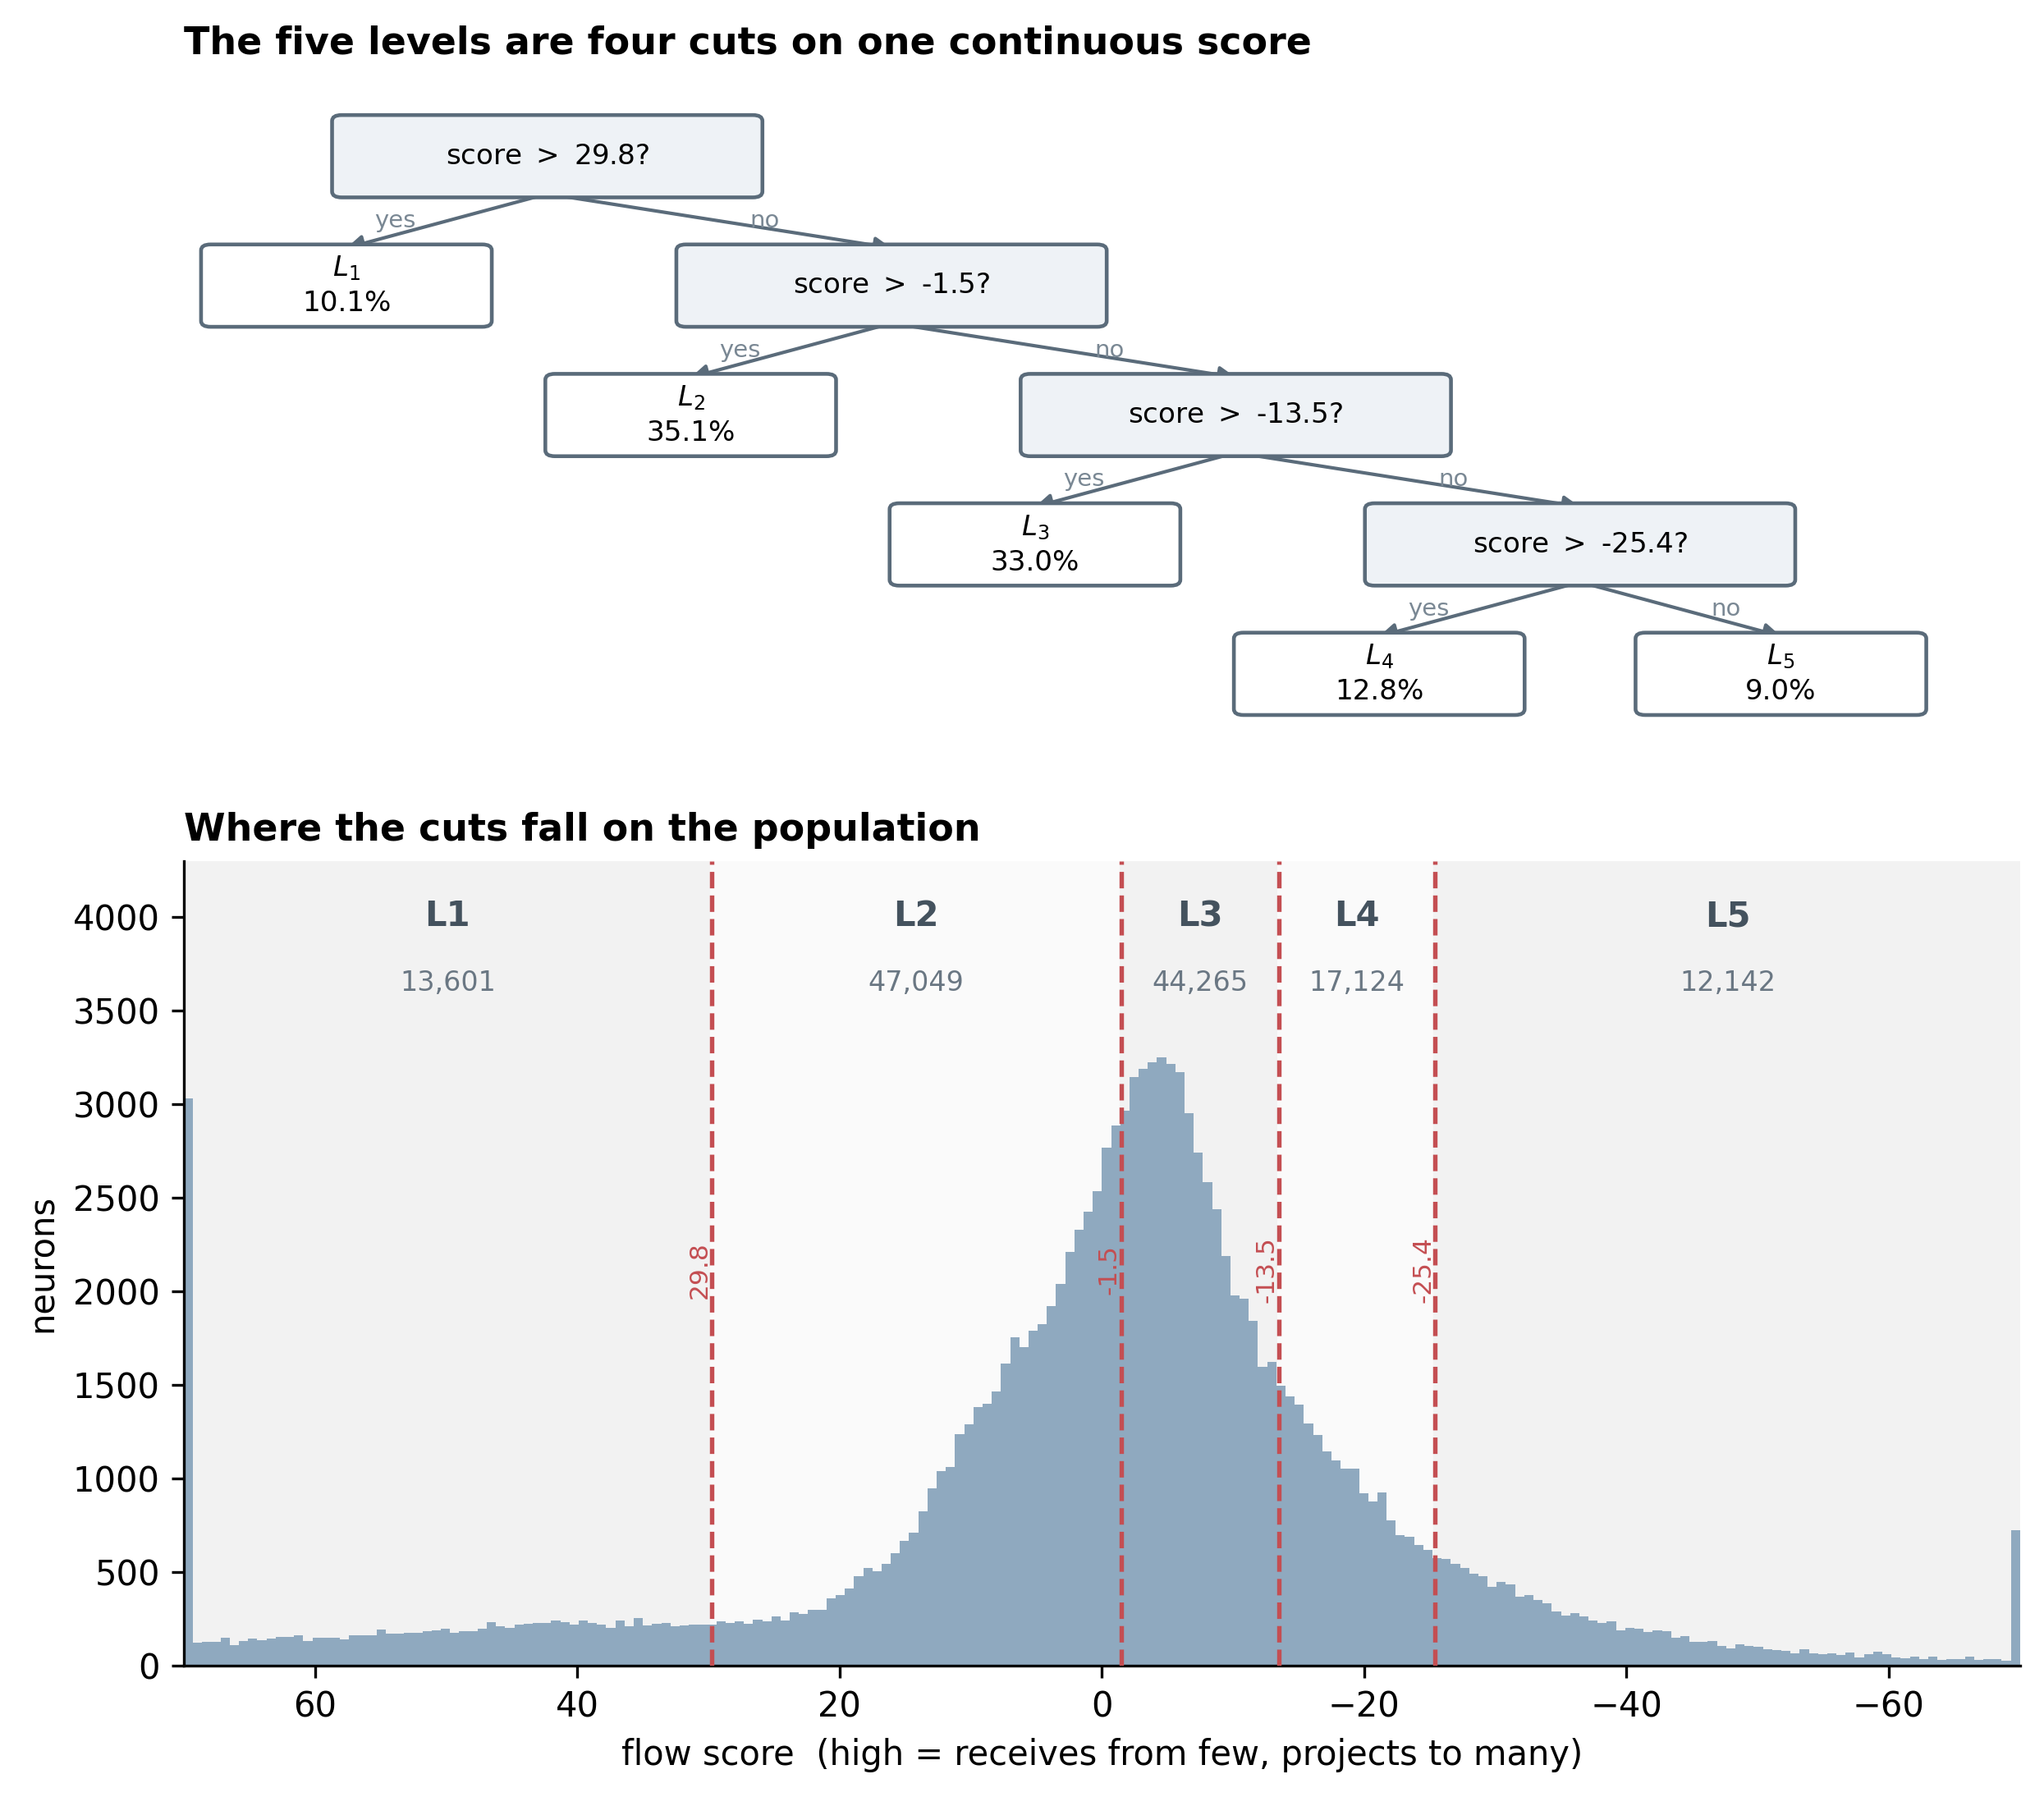
\includegraphics[width=0.92\textwidth]{level_construction.png}
\caption[How the hierarchical levels are constructed]{How the five levels are
obtained. Above, the decision tree: because all four thresholds apply to the
same quantity, the tree is a comb in which each test peels off one level and
passes the remainder to the next, and the percentages are the share of the
$134{,}181$ neurons falling in each. Below, the same four cuts drawn on the
distribution of the flow score itself, with the score increasing to the left
so that the sensory end of the axis is on the left and the motor end on the
right; the bars at the extremes collect the tails, which run to $906$ and
$-306$. The two central levels are the populous ones, and the cut between
them falls almost exactly on the peak of the distribution.}
\label{fig:level-construction}
\end{figure}

Two things are worth noticing in that figure, because they explain results
that appear later. The distribution is heavily concentrated near the middle
of the axis, so levels~2 and~3 together hold $68\%$ of the neurons, and the
boundary between them cuts through the densest part of the population rather
than through a gap. Neither fact is a defect of the construction: a
continuous axis has no gaps to cut at, which is precisely why a criterion
external to the geometry, namely the super-class, is needed to place the
boundaries at all.

This has a consequence that matters for the next section. Since the cut
points were chosen to separate super-classes, levels and super-classes are
not independent, and pairing them is in one sense the natural thing to do.
This thesis nevertheless groups neurons more finely, for reasons set out in
Section~\ref{sec:groups}, and the cost of that choice is measured rather
than assumed.

Once levels are available, every edge acquires a direction relative to the
hierarchy. For an edge running from a neuron at level $y_u$ to a neuron at
level $y_v$ we write
\begin{equation}
  \label{eq:edge-direction}
  \mathrm{dir}(u,v) =
  \begin{cases}
    \mathrm{FWD} & \text{if } y_u < y_v \quad \text{(forward)},\\
    \mathrm{BWD} & \text{if } y_u > y_v \quad \text{(backward)},\\
    \mathrm{LAT} & \text{if } y_u = y_v \quad \text{(lateral)}.
  \end{cases}
\end{equation}
A forward edge carries information deeper into the hierarchy, a backward
edge returns it towards the periphery, and a lateral edge moves it sideways
within a single processing stage. This three-way classification is used
throughout the thesis and underlies the finer signature scheme introduced in
Section~\ref{sec:motifs}.

A remark on notation is needed here, because the natural abbreviations are
not available. The two directions would ordinarily be written FF for
feed-forward and FB for feedback, and this is how they appear in much of the
network-motif literature. In this connectome the second of those collides
with an anatomical name: \code{FB} is the standard abbreviation of the
fan-shaped body, a neuropil of the central complex, and it occurs in nineteen
of the anatomical groups set out in Section~\ref{sec:nomenclature}; it also
appears in this thesis, in Table~\ref{tab:within-null}, as an area rather
than as a direction. A reader who meets \code{BWD->FWD} without the glossary at
hand has no way of telling which of the two is meant. The abbreviations used
for directions are therefore \code{FWD}, \code{BWD} and \code{LAT}, which
collide with nothing, and the anatomical codes keep their usual meaning. In
running text the three are called forward, backward and lateral; the terms
\emph{feed-forward} and \emph{feedback} are kept for the general notions as
they appear in the literature, and are not used as names for the classes
measured here.

\subsubsection{The Anatomical Nomenclature}
\label{sec:nomenclature}

Every result in this thesis names anatomical structures by abbreviation, and
those abbreviations are not arbitrary labels: they follow a system that is
worth setting out before any of them appears in a figure, since a reader who
does not know it cannot interpret a single pattern.

The insect brain is divided into \emph{neuropils}, dense regions of
synaptic connections separated by tracts of fibres, and the standard
nomenclature of Ito et al.\ \cite{ito2014} assigns each one a short
uppercase code. FlyWire annotates every neuron with the set of neuropils in
which it \emph{arborises}, that is, in which its branches spread out and make
synapses, and this annotation is the \code{group} field of the dataset. The field has $628$ distinct values, which sounds unmanageable
until one sees how they are built. There are only $44$ distinct neuropils in
the annotation, and a group is either a single neuropil, of which there are
$44$, or a pair of neuropils written with a dot between them, of which there
are $584$. No group names more than two. So \code{ME} is a neuron confined to
the medulla, \code{LO} one confined to the lobula, and \code{ME.LO} a neuron
that arborises in both and therefore connects them; \code{AL.MB\_CA} spans
the antennal lobe and the mushroom body calyx, which is the anatomical
signature of an olfactory \emph{projection neuron}, a neuron whose branches
span two regions and which therefore carries signals from one to the other.
Reading a group name is thus a
matter of reading at most two codes, and the dot should be understood as
``and'', not as a hierarchy.

Three of these neuropils deserve a word on their own, because they carry
most of the results reported later. The \emph{medulla}, the \emph{lobula} and
the \emph{lobula plate} are three successive stages of the optic lobe: light
is transduced in the retina, passes to the lamina and then to the medulla,
which is the largest neuropil in the brain and performs the first substantial
visual computation; from there information splits into two parallel streams,
one reaching the lobula, associated with the analysis of form and features,
and one reaching the lobula plate, which is the stage specialised for
detecting motion. A pattern such as \code{ME.LO} therefore names a neuron
bridging two consecutive stages of this pathway, and a circuit running from
medulla groups through the lobula to the lobula plate is a circuit moving
from early visual processing into motion analysis. The olfactory counterpart
is the chain from the \emph{antennal lobe}, which receives input from the
smell receptors, to the \emph{mushroom body}, the centre for olfactory
learning, and the \emph{lateral horn}, which mediates innate rather than
learned responses to odours.

The $44$ neuropils are themselves organised into thirteen \emph{super-regions}
in the same nomenclature, and this grouping is the macro-level of the
anatomy. The medulla, lobula, lobula plate, lamina and accessory medulla make
up the optic lobe; the fan-shaped body, ellipsoid body, protocerebral bridge
and noduli make up the central complex; the calyx, pedunculus and the two
lobes make up the mushroom body; and so on through the superior, inferior,
ventrolateral, ventromedial and periesophageal neuropils. Table~\ref{tab:neuropils}
gives the complete list with the population of each, grouped by super-region.
The super-regions matter here for two reasons: they let a reader place an
unfamiliar code without consulting an atlas, and they define a third
granularity, intermediate between the nine functional super-classes and the
$628$ groups, which Section~\ref{sec:results-granularity} uses as a control.

The two halves of this description have different standing, and it is worth
separating them. The neuropil codes themselves are carried by the data: the
per-synapse annotation of the connection table names the same forty-four
regions, in hemisphere-resolved form, and the tokens appearing in the
\code{group} field are exactly those. The assignment of neuropils to
super-regions, by contrast, is not a field of the dataset at all; it is the
hierarchy of the published nomenclature, applied here. Nothing in the data
would reveal an error in it, so it is stated as a convention taken from
\cite{ito2014} rather than as a measurement.

% [t] e non [H]: con [H] la tabella non entrava nella pagina in corso e la
% spezzava, lasciando tre quarti di pagina bianchi prima di lei
\begin{table}[t]
\centering
\caption[The 44 neuropils of the annotation]{The $44$ neuropils that compose
the \code{group} annotation, grouped by super-region and ordered by
population within each. The counts divide a neuron between the two neuropils
of a composite group, so they sum to the $134{,}181$ neurons that carry both
a group and a level. Any group name in this thesis is one of these codes or
two of them joined by a dot.}
\label{tab:neuropils}
\scriptsize
\begin{minipage}[t]{0.49\textwidth}
\vspace{0pt}
\centering
\begin{tabular}{llr}
\toprule
Code & Name & Neurons \\
\midrule
\multicolumn{3}{l}{\textit{Optic Lobe}} \\
\code{ME} & Medulla & 55{,}811 \\
\code{LO} & Lobula & 18{,}231 \\
\code{LOP} & Lobula Plate & 8{,}669 \\
\code{LA} & Lamina & 7{,}157 \\
\code{AME} & Accessory Medulla & 36 \\
\midrule
\multicolumn{3}{l}{\textit{Ocellar Ganglion}} \\
\code{OCG} & Ocellar Ganglion & 274 \\
\midrule
\multicolumn{3}{l}{\textit{Antennal Lobe}} \\
\code{AL} & Antennal Lobe & 3{,}048 \\
\midrule
\multicolumn{3}{l}{\textit{Lateral Horn}} \\
\code{LH} & Lateral Horn & 2{,}121 \\
\midrule
\multicolumn{3}{l}{\textit{Mushroom Body}} \\
\code{MB\_CA} & Mushroom Body Calyx & 2{,}440 \\
\code{MB\_ML} & Mushroom Body Medial Lobe & 2{,}002 \\
\code{MB\_VL} & Mushroom Body Vertical Lobe & 484 \\
\code{MB\_PED} & Mushroom Body Pedunculus & 246 \\
\midrule
\multicolumn{3}{l}{\textit{Central Complex}} \\
\code{FB} & Fan-shaped Body & 1{,}728 \\
\code{EB} & Ellipsoid Body & 382 \\
\code{NO} & Noduli & 376 \\
\code{PB} & Protocerebral Bridge & 108 \\
\midrule
\multicolumn{3}{l}{\textit{Lateral Complex}} \\
\code{LAL} & Lateral Accessory Lobe & 981 \\
\code{BU} & Bulb & 31 \\
\code{GA} & Gall & 12 \\
\midrule
\bottomrule
\end{tabular}
\end{minipage}\hfill
\begin{minipage}[t]{0.49\textwidth}
\vspace{0pt}
\centering
\begin{tabular}{llr}
\toprule
Code & Name & Neurons \\
\multicolumn{3}{l}{\textit{Superior Neuropils}} \\
\code{SMP} & Superior Medial Protocerebrum & 3{,}458 \\
\code{SLP} & Superior Lateral Protocerebrum & 3{,}150 \\
\code{SIP} & Superior Intermediate Protocerebrum & 443 \\
\midrule
\multicolumn{3}{l}{\textit{Inferior Neuropils}} \\
\code{ICL} & Inferior Clamp & 980 \\
\code{CRE} & Crepine & 920 \\
\code{SCL} & Superior Clamp & 408 \\
\code{IB} & Inferior Bridge & 268 \\
\code{ATL} & Antler & 65 \\
\midrule
\multicolumn{3}{l}{\textit{Ventrolateral Neuropils}} \\
\code{AVLP} & Anterior Ventrolateral Protocerebrum & 3{,}682 \\
\code{PLP} & Posterior Lateral Protocerebrum & 2{,}274 \\
\code{PVLP} & Posterior Ventrolateral Protocerebrum & 1{,}607 \\
\code{AOTU} & Anterior Optic Tubercle & 926 \\
\code{WED} & Wedge & 408 \\
\midrule
\multicolumn{3}{l}{\textit{Ventromedial Neuropils}} \\
\code{IPS} & Inferior Posterior Slope & 1{,}604 \\
\code{SPS} & Superior Posterior Slope & 1{,}534 \\
\code{VES} & Vest & 432 \\
\code{GOR} & Gorget & 70 \\
\code{EPA} & Epaulette & 10 \\
\midrule
\multicolumn{3}{l}{\textit{Periesophageal Neuropils}} \\
\code{SAD} & Saddle & 968 \\
\code{PRW} & Prow & 593 \\
\code{AMMC} & Antennal Mechanosensory and Motor Centre & 513 \\
\code{FLA} & Flange & 334 \\
\code{CAN} & Cantle & 8 \\
\midrule
\multicolumn{3}{l}{\textit{Gnathal Ganglia}} \\
\code{GNG} & Gnathal Ganglia & 5{,}379 \\
\midrule
\multicolumn{3}{l}{\textit{Unassigned}} \\
\code{UNASGD} & Unassigned & 10 \\
\bottomrule
\end{tabular}
\end{minipage}
\end{table}

\subsubsection{Group-Level Abstraction}
\label{sec:groups}

Counting motifs over individual neurons is both computationally hopeless and
biologically uninformative. It is hopeless because a five-node motif over
$134{,}000$ nodes has astronomically many candidate instantiations, and
uninformative because individual neurons are not the units at which circuit
function is usually described: what one wants to know is that the antennal
lobe projects to the mushroom body calyx, not that one particular neuron
does.

We therefore abstract from neurons to \emph{metanodes}. A metanode is a pair
consisting of an anatomical category and a hierarchical level, so that the
neurons of one structure sitting at level~2 form one metanode and those of
the same structure at level~3 form another. A motif is then a pattern over
metanodes, and its count is the number of distinct neuron-level
instantiations of that pattern. This preserves the quantity that actually
matters, namely how many real circuits realise the pattern, while reducing
the search space by several orders of magnitude.

Two quantities derived from these counts are used throughout the results and
are worth naming now, because they answer different questions and frequently
disagree. The \emph{number of patterns} in a set is how many distinct
metanode configurations it contains, each counted once however often it
occurs. The \emph{mass} of that set is the sum of the counts of its patterns,
that is, the total number of neuron-level circuits realising any of them. A
class of motifs may contain very many distinct patterns that are each rare,
giving it a large number of patterns and a small mass, or a handful of
patterns that are each realised enormously often, giving the reverse. Both
are reported wherever the two diverge, and percentages are stated as shares
of one or the other, never of an unspecified total.

Which categorisation to use is a real choice, and three are available.

The coarsest is the \emph{super-class}, a functional label carried by the
FlyWire classification and taking nine values. Since these names recur
throughout the results, and since three of them concern the visual system
specifically and are easy to confuse, they are set out here.
\emph{Sensory} neurons carry signals into the brain from the sense organs.
\emph{Optic} neurons lie within the optic lobe, the large visual region that
occupies most of each side of the head, and process visual input locally.
\emph{Visual projection} neurons carry visual information \emph{out} of the
optic lobe towards the central brain, and \emph{visual centrifugal} neurons
run the other way, carrying signals from the central brain back \emph{into}
the optic lobe. \emph{Central} neurons lie in the central brain and are
neither sensory nor motor: this is where association, learning and
decision-making happen. \emph{Descending} neurons carry commands out of the
brain towards the nerve cord that drives the body, \emph{ascending} neurons
carry signals up from the nerve cord into the brain, \emph{motor} neurons
drive muscles directly, and \emph{endocrine} neurons release hormones rather
than acting on a specific target. The
finest is the \emph{anatomical group} of Section~\ref{sec:nomenclature},
which takes $628$ values. Between them sits the \emph{super-region}, obtained
by replacing each neuropil of a group with the super-region that contains it,
so that \code{ME.LO} becomes \code{OL}, both of its neuropils lying in the
optic lobe, while \code{LO.PLP} becomes \code{OL.VLNP}, its two neuropils
lying in different super-regions; this yields $79$ values.

Paired with the five levels, the three give metanode sets that differ by
almost two orders of magnitude. On the shallow window they give $24$, $188$
and $879$ metanodes respectively, with median populations of $511$, $11$ and
$3$ neurons and metagraphs of $293$, $6{,}295$ and $24{,}914$ edges.
Figure~\ref{fig:metagraph} shows the coarsest graph in full and the
distribution of metanode sizes.

This thesis uses the \emph{anatomical group}. The reason is that the question
being asked is which \emph{structure} occupies the waist, and the super-class
label cannot express an answer to it: the category \emph{central} alone
collapses $521$ distinct anatomical groups into one node. The antennal lobe
projection neurons, which carry odour information from the antennal lobe to
the mushroom body; the Kenyon cells, which are the numerous small neurons
forming the body of the mushroom body itself and on which odour memories are
stored; and the mushroom body output neurons, which read that structure out
towards behaviour, are all, without exception, \emph{central}; so is the
lateral horn.  Any statement about how information is routed within the
central brain is therefore unavailable at that granularity, by construction
rather than by accident.

The cost of the finer choice is a long tail of very small categories. The
median group holds eight neurons across the whole connectome and the median
metanode three on the shallow window, and $344$ of the $628$ groups hold
fewer than ten neurons each. Stated that way the abstraction sounds far too
specific to support any general claim, which is why it is worth stating the
other half of the same distribution: those $344$ small groups together
account for $0.8\%$ of the neurons, and $99.2\%$ of the population lives in
groups of ten neurons or more. The median is low because the tail is long,
not because the analysis rests on tiny categories. The
$\mathit{min\_count}$ threshold of Section~\ref{sec:micro-methods} then
removes any pattern supported by fewer than ten instances, so the small
categories that do exist are also the ones least likely to survive into a
reported result. What remains a genuine limitation is that no threshold can
make a category informative if it was small to begin with, and
Section~\ref{sec:results-granularity} repeats the entire analysis at both of
the coarser granularities in order to measure what that costs.

\begin{figure}[H]
\centering
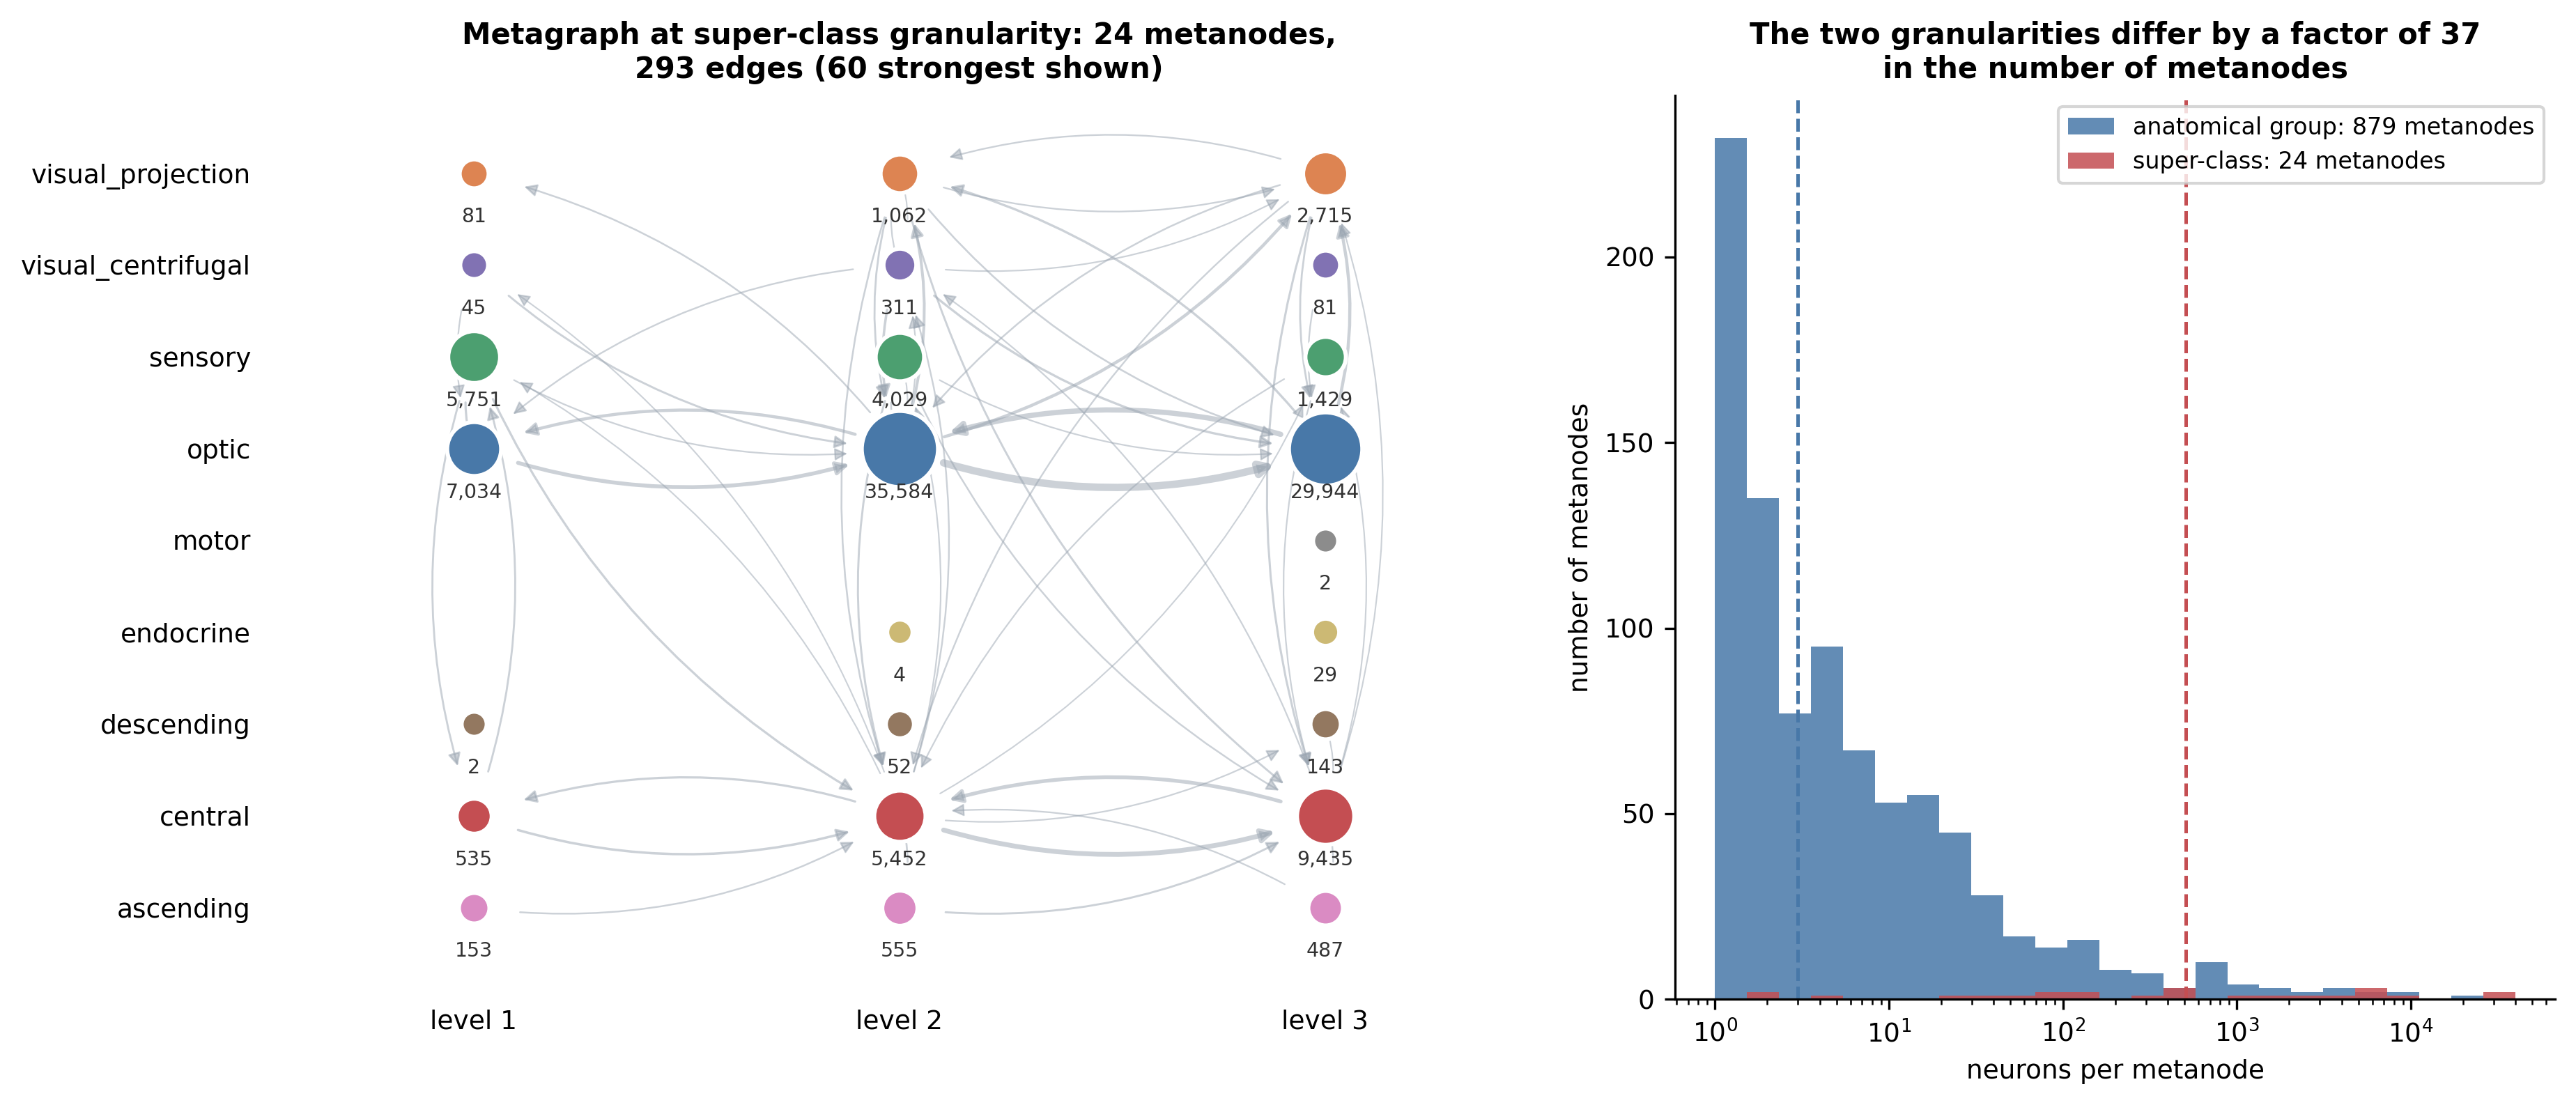
\includegraphics[width=\textwidth]{metagraph.png}
\caption[The metagraph at two granularities]{The metagraph on which motifs
are counted. On the left, the graph at super-class granularity for window
$\{1,2,3\}$: each node is a metanode, that is a (super-class, level) pair,
placed by level on the horizontal axis and sized by the number of neurons it
contains; the sixty strongest of its $293$ edges are drawn. On the right, the
distribution of metanode populations under the two categorisations, with
medians marked. The group-level metagraph has $879$ nodes and $24{,}914$
edges and cannot be drawn legibly, which is itself an indication of the
difference in resolution between the two.}
\label{fig:metagraph}
\end{figure}

\subsection{Network Motifs}
\label{sec:motifs}


A motif is a small connectivity pattern that occurs more often than chance
would predict. This section defines the idea, explains why the comparison
against chance is part of the definition rather than an afterthought, and
introduces the scheme by which the patterns of this thesis are classified
according to the direction their edges run in the hierarchy. That
classification is used continuously from here on, so it is developed in full
here rather than where the results first need it.

\subsubsection{Motifs as Building Blocks}

Milo et al.\ \cite{milo2002} introduced network motifs as patterns of
interconnection that recur in a network significantly more often than they
do in randomised networks preserving specified properties. The significance
requirement is what distinguishes a motif from a merely frequent subgraph,
and it is essential: a pattern may be common simply because the network is
dense, or because certain nodes happen to have very high degree, without
that frequency reflecting anything about the organisation of the system. The
comparison against a randomised ensemble is therefore not a statistical
formality added at the end but part of the definition, and
Section~\ref{sec:validation-methods} describes the three ensembles used
here.

\subsubsection{Directional Classification}

Given the level assignment, every edge of a motif carries one of the three
directions of Equation~\eqref{eq:edge-direction}. A bow-tie motif with two
input groups and two output groups has four edges, two entering the waist
and two leaving it. Rather than labelling the motif by all four edges
individually, which would produce an unwieldy number of categories, we
classify each \emph{branch} by whether its edges agree with one another. If
both edges entering the waist are forward, the input branch is labelled
\code{FWD}; if they disagree, it is labelled \emph{mix}. The same applies to the
output branch. The resulting label is written
\begin{equation}
  \label{eq:signature}
  \mathrm{signature} = \mathrm{sig}_{\mathrm{in}} \rightarrow
                       \mathrm{sig}_{\mathrm{out}},
  \qquad
  \mathrm{sig} \in \{\mathrm{FWD},\mathrm{BWD},\mathrm{LAT},\mathrm{mix}\},
\end{equation}
which yields sixteen possible signatures. A motif labelled
\code{FWD->LAT}, for instance, is one in which two groups feed forward onto a
waist that then distributes laterally within its own level.
Figure~\ref{fig:signature-grid} draws all sixteen.

% [H] e non [t]: e' troppo alta per stare in cima a una pagina, quindi come
% float verrebbe rimandata fino in fondo al documento. La coda bianca sulla
% pagina precedente e' il prezzo da pagare per tenerla dove la si cita.
\begin{figure}[H]
\centering
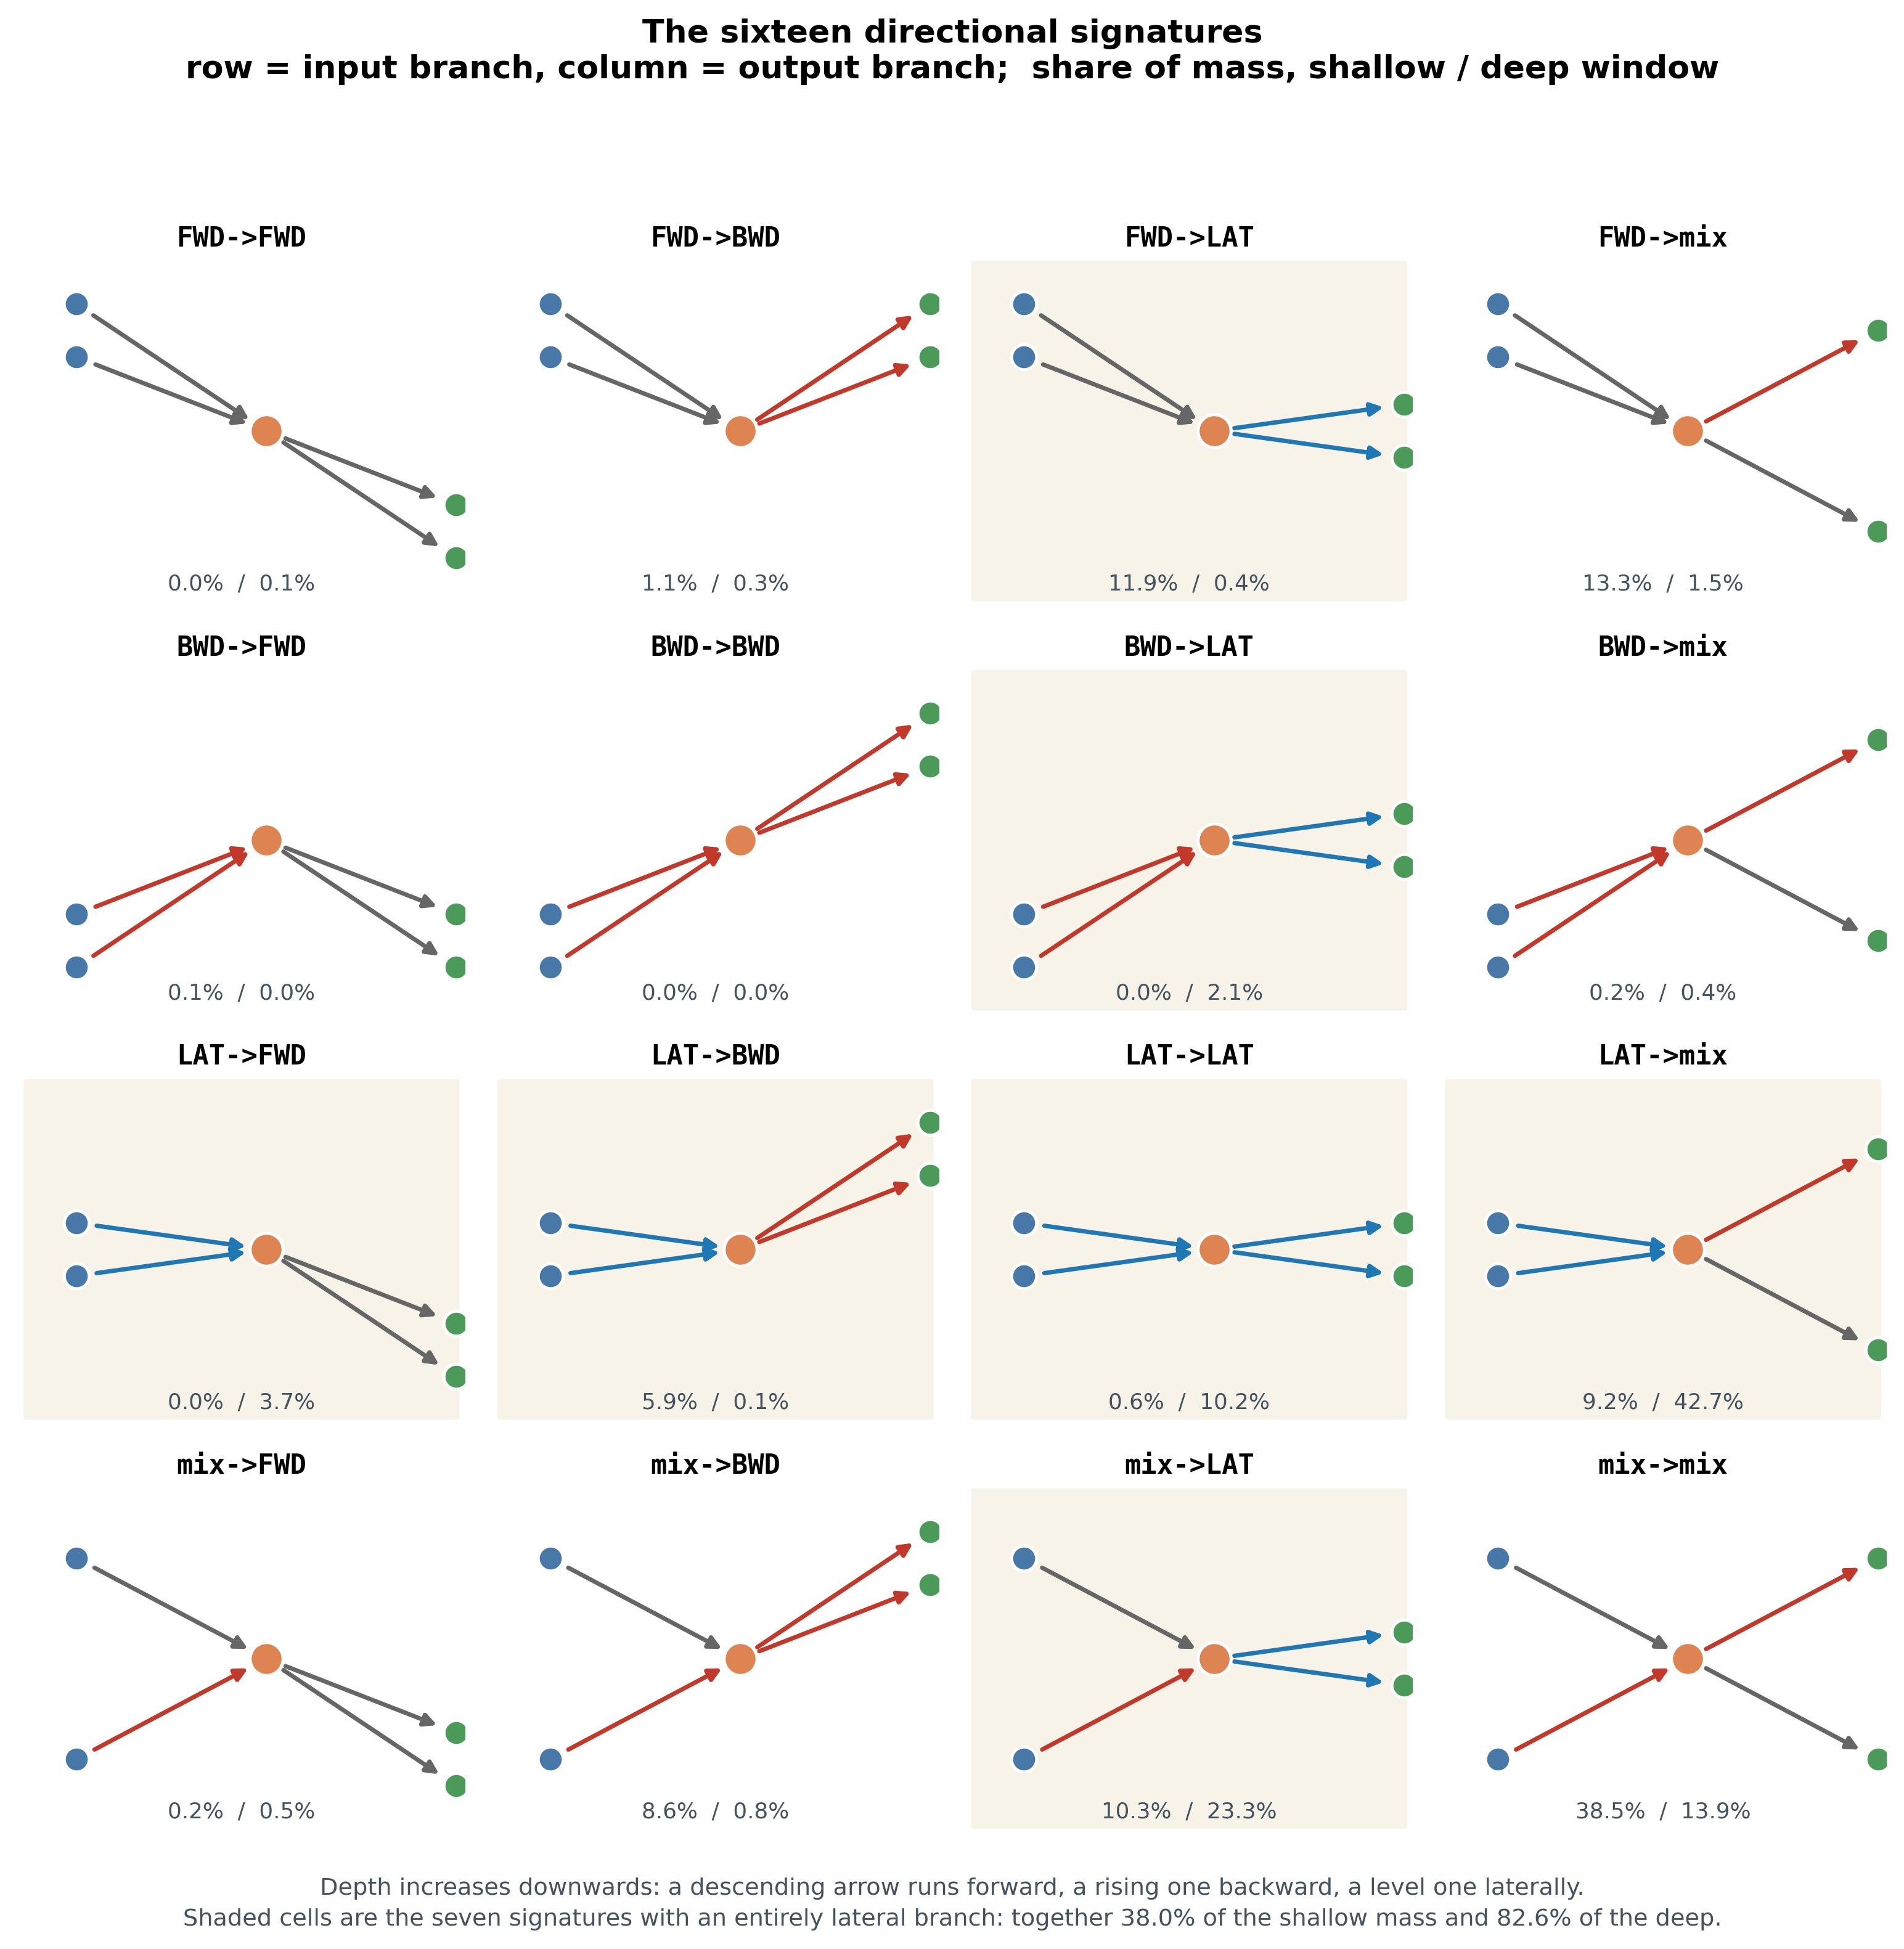
\includegraphics[width=0.98\textwidth]{signature_grid.png}
\caption[The sixteen directional signatures]{The sixteen signatures, laid
out as a matrix: the row gives the direction of the input branch and the
column that of the output branch. Depth increases downwards, so the
direction of a branch can be read from the slope of its arrows, and a
\emph{mix} branch is drawn with one arrow of each kind. Beneath each cell
are the shares of motif mass in the shallow and deep windows, from
Table~\ref{tab:signatures}. The shaded cells are the seven signatures in
which at least one branch is entirely lateral; the contrast between their
two numbers is the shift reported in
Section~\ref{sec:results-signature}.}
\label{fig:signature-grid}
\end{figure}

It is worth being explicit about why the signature is defined at this level
of detail rather than more simply, because the alternative was tried first
and does not work.

The obvious classification, and the one used in earlier work on this dataset,
labels a motif by the agreement of all four of its edges at once: a motif is
\emph{pure\_FWD}, \emph{pure\_BWD} or \emph{pure\_LAT} when every edge runs
the same way, and \emph{mixed} otherwise. The difficulty is arithmetic. Four
edges each running in one of three directions give $81$ possible
combinations, of which only three have all four in agreement, so complete
agreement is improbable before one looks at any data at all. On the shallow
window the outcome is what that arithmetic predicts: $29{,}453{,}022$
patterns, $94.4\%$ of the total, fall into \emph{mixed}, while
\emph{pure\_LAT} takes $1{,}651{,}892$ ($5.3\%$), \emph{pure\_FWD}
$57{,}821$ ($0.19\%$) and \emph{pure\_BWD} only $22{,}065$ ($0.07\%$). A
label that assigns nineteen patterns in twenty to a single class is not
telling us much about the connectome; it is telling us that four independent
things rarely agree.

The signature of Equation~\eqref{eq:signature} avoids this by asking for
agreement within each branch separately rather than across the motif as a
whole. Two edges agree far more often than four, so the classes it produces
are populated rather than empty, and the thirteen classes hiding inside
\emph{mixed} turn out to behave very differently from one another. This is
why the finer scheme is used throughout, and why the coarse label appears in
this thesis only where a comparison with earlier work requires it.

\subsection{Bow-Tie and Hourglass Architecture}
\label{sec:hourglass-theory}


This section defines the two structures the thesis is about and separates
them, because the literature often does not. The bow-tie is a local pattern
and is defined precisely enough to be counted; the hourglass is a global
property of a network and is defined precisely enough to be measured. The
distinction is what makes it meaningful to ask, later, whether the two
agree.

\subsubsection{The Bow-Tie Motif}

\begin{definition}[Bow-tie motif]
\label{def:bowtie}
Given metanodes $A_1,\dots,A_{\kin}$, a waist metanode $B$, and metanodes
$D_1,\dots,D_{\kout}$, with
$\{A_m\} \cap \{D_n\} = \emptyset$ and $B \notin \{A_m\} \cup \{D_n\}$, a
bow-tie motif instance is a tuple of distinct neurons
$(a_1,\dots,a_{\kin}, b, d_1,\dots,d_{\kout})$ with $a_m \in A_m$,
$b \in B$, $d_n \in D_n$, such that $(a_m, b) \in E$ for all $m$ and
$(b, d_n) \in E$ for all $n$.
\end{definition}

Figure~\ref{fig:bowtie-schema} shows the structure schematically. The
requirement that the input and output groups be disjoint deserves particular
emphasis, because it is easy to omit and expensive to omit. Without it a
metanode may appear simultaneously among the inputs and the outputs of the
same motif, so that what is counted is not a bow-tie at all but a
configuration in which a group feeds back into itself through the waist.
Such configurations are extremely numerous, because the same group
reappearing on both sides multiplies the available combinations, and they
are also degenerate in the sense that they do not describe convergence
followed by divergence. Enforcing the constraint removes $6.60\%$ of the patterns but $57.3\%$ of
the total count mass, which gives a measure of how strongly degenerate
configurations dominate when the search is left unconstrained.

\begin{figure}[H]
\centering
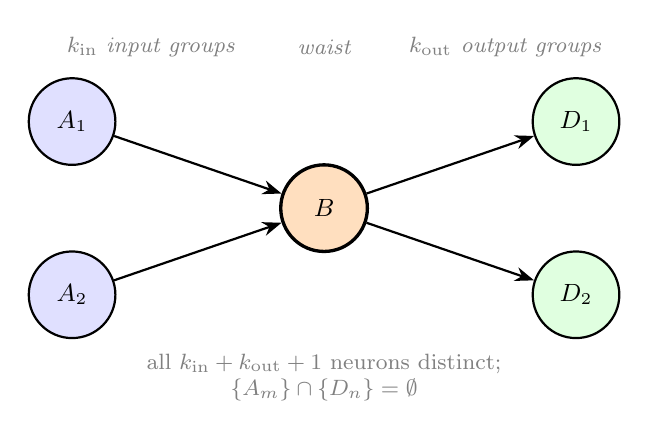
\begin{tikzpicture}[
  >={Stealth[length=2.4mm]},
  grp/.style={circle,draw,thick,minimum size=11mm,inner sep=0pt,font=\small},
  inp/.style={grp,fill=blue!12},
  wst/.style={grp,fill=orange!25,very thick},
  outg/.style={grp,fill=green!12},
  lab/.style={font=\footnotesize\itshape,gray}
]
  \node[inp] (a1) at (0,1.1)  {$A_1$};
  \node[inp] (a2) at (0,-1.1) {$A_2$};
  \node[wst] (b)  at (3.2,0)  {$B$};
  \node[outg] (d1) at (6.4,1.1)  {$D_1$};
  \node[outg] (d2) at (6.4,-1.1) {$D_2$};

  \draw[->,thick] (a1) -- (b);
  \draw[->,thick] (a2) -- (b);
  \draw[->,thick] (b) -- (d1);
  \draw[->,thick] (b) -- (d2);

  \node[lab] at (1.0,2.05) {$\kin$ input groups};
  \node[lab] at (3.2,2.05) {waist};
  \node[lab] at (5.5,2.05) {$\kout$ output groups};

  \node[font=\footnotesize,gray,align=center] at (3.2,-2.15)
    {all $\kin+\kout+1$ neurons distinct;\\
     $\{A_m\} \cap \{D_n\} = \emptyset$};
\end{tikzpicture}
\caption[The bow-tie motif]{The bow-tie motif of
Definition~\ref{def:bowtie}. Each node is a metanode, that is, a pair
consisting of an anatomical group and a hierarchical level; an instance of
the motif is a tuple of distinct neurons, one drawn from each metanode,
connected as shown. The disjointness requirement between input and output
groups is what prevents degenerate configurations in which a group feeds
back into itself through the waist.}
\label{fig:bowtie-schema}
\end{figure}

\subsubsection{The Hourglass Effect}

Sabrin et al.\ \cite{sabrin2020} formalise the hourglass property of a
hierarchical network in three steps. One begins by fixing a set $S$ of
source nodes and a set $T$ of target nodes; in a connectome these are
naturally the sensory and the motor neurons respectively. For each node $v$
of the network one then computes its \emph{path centrality}, defined as the
number of source-to-target paths that traverse $v$. Ordering all nodes by
decreasing path centrality and taking the smallest prefix of that ordering
which together covers a fraction $\tau$ of all source-to-target paths yields
the \emph{$\tau$-core}, written $C(\tau)$. Intuitively, the $\tau$-core is
the smallest set of neurons through which most of the traffic must pass.

A small core is not by itself evidence of an hourglass, and this is the
point at which the framework becomes subtle. A network might have a small
core simply because its source-to-target dependencies are themselves
concentrated, quite apart from any hierarchical organisation. The comparison
is therefore made against the \emph{flat dependency network}, constructed by
connecting every source directly to every target it can reach and discarding
all intermediate structure. This flat network has exactly the same
dependencies as the original but no hierarchy whatsoever. Writing
$C_f(\tau)$ for its core, the hourglass score is
\begin{equation}
  \label{eq:hscore}
  H = 1 - \frac{|C(\tau)|}{|C_f(\tau)|} .
\end{equation}
A value of $H$ close to $1$ means that the real network routes its flow
through far fewer intermediaries than its dependency structure requires,
which is the signature of an hourglass. A value close to $0$ means that the
apparent concentration is entirely explained by the dependencies themselves
and that the hierarchy contributes nothing.

\subsection{Previous Work}
\label{sec:related}

Two recent theses prepared under the same supervision analyse the same
connectome with complementary aims. Tricoli \cite{tricoli2025} studies
neuronal assemblies through motif-based characterisation combined with
hierarchical flow ranking, with the goal of identifying groups of neurons
that share structural roles and might therefore act as functional units.
Curcio \cite{curcio2026} introduces a parametric framework for motif
discovery conditioned on hierarchical position, and explores the resulting
search space along three axes: the vertical depth of the window, the
horizontal complexity of the pattern, and the distance spanned by
skip connections.

Both of those works enumerate motifs of fixed size and interpret them in
terms of super-class composition. The present thesis differs from them in
three respects. It targets one specific architectural template, the bow-tie,
rather than attempting a full motif census, and this restriction is what
makes exact counting through a closed formulation possible where enumeration
would not be. It pairs the local analysis with a global hourglass
measurement and then quantifies the agreement between the two rather than
reporting either in isolation. And it treats statistical validation and
the fate of unconfirmed hypotheses as first-class outputs, on the view that
an analysis whose controls are not reported cannot be assessed by a reader.

Earlier work on the larval connectome of the same species
\cite{corradini2025} treated the brain as a flat homogeneous graph and
enumerated motifs without conditioning on hierarchical position at all,
which produces useful global statistics but collapses together circuits
operating at very different processing stages. The present work uses the
adult connectome, in which the number of neurons is larger by an order of
magnitude, so the contrast is one of method rather than a direct
comparison of results.

%=======================================================================
\section{Methods}
\label{sec:methods}

The two questions of the previous chapter are answered at two different
scales, and this chapter describes the machinery for both, in the order in
which the results are later presented: the global question first, then the
local one.

The order matters and is worth justifying. Asking which structures form
waists only makes sense once one knows whether the network has an hourglass
organisation at all; and a measurement of that global organisation is
interpretable on its own, whereas a catalogue of local patterns is not,
since any large network contains many patterns of any given shape. The
global analysis therefore comes first and sets the terms, the local one then
identifies the structures responsible, and Section~\ref{sec:results-bridge}
compares what the two say about the same tissue.

Both rest on the same foundation, which is why it is described before either.
Section~\ref{sec:counting} develops a way of counting how many times a
pattern occurs without ever enumerating its occurrences, by exploiting the
fact that a count over a branching pattern factorises into a product over
the point where the branches meet. That single idea is applied twice: to the
waist of a bow-tie, where it gives the number of local patterns, and to a
node of the whole network, where it gives the number of sensory-to-motor
paths through it. The chapter then covers the statistical validation that
distinguishes a motif from a merely frequent pattern, the engineering that
makes an exhaustive count feasible, and the checks that establish that the
counts are right.
%=======================================================================

\subsection{Counting Without Enumeration}
\label{sec:counting}


Everything in this thesis rests on being able to count occurrences of a
pattern without listing them, because at connectome scale the occurrences
number in the hundreds of billions and listing them is not an option. This
section develops that capability in four steps: it recasts pattern counting
as a linear-algebraic operation, extends it from chains to branching
patterns, establishes exactly which patterns the extension covers, and
verifies the resulting formulae against brute-force enumeration. The fourth
step also fixes the limits of the method, which are as important to state as
its reach.

\subsubsection{Homomorphism Counting and Flow Vectors}

Counting the occurrences of a pattern $P$ in a graph $G$ amounts to counting
the homomorphisms from $P$ into $G$ that respect the prescribed group
memberships. A homomorphism here is simply an assignment of a neuron to each
node of the pattern such that every edge of the pattern is realised by an
edge of the graph. For a pattern that is a \emph{path} this reduces to
Equation~\eqref{eq:path-count}: one propagates a vector along the pattern
through a sequence of sparse matrix--vector products, and the total count
falls out at the end. The vector being propagated is called the \emph{flow
vector}, and its $i$-th entry has a direct interpretation as the number of
partial matches of the pattern that terminate at neuron $i$.

The propagation of the flow vector along a chain of groups follows the
implementation of Curcio \cite{curcio2026}, from which this part of the code
derives; the extension to branching patterns developed in
Section~\ref{sec:sigmapi} is specific to the present work.

The flow vector has a property that turns out to be decisive. Because the
operation is linear, the count computed over a union of groups equals the
sum of the counts computed over the individual groups. Counting the pattern
on $A_1 \cup A_2$ therefore requires no more work than counting it on $A_1$
and on $A_2$ separately and adding the results. This is what allows a search
to consider large collections of groups without the cost growing with the
number of combinations of them.

\subsubsection{The \sigmapi{} Formulation}
\label{sec:sigmapi}

A bow-tie is not a path. It is a tree with a branching point at the waist,
and at that branching point the two incoming branches are required to be
incident on the \emph{same} neuron. That requirement is what destroys the
linearity, because the count of the combined pattern is no longer determined
by the counts of its parts: knowing how many neurons of $A_1$ reach the
waist and how many neurons of $A_2$ reach it does not tell us how many
neurons of the waist are reached by both.

The correct formulation must therefore work neuron by neuron across the
waist. Let $v_{A_m}[i]$ denote the number of neurons of group $A_m$ that
project onto neuron $i$ of the waist, and let $w_{D_n}[i]$ denote the number
of neurons of group $D_n$ that receive from that same neuron $i$. Then the
exact count of the bow-tie is
\begin{equation}
  \label{eq:sigmapi}
  c(A_1,\dots,A_{\kin};B;D_1,\dots,D_{\kout})
  \;=\;
  \sum_{i \in B}
  \left( \prod_{m=1}^{\kin} v_{A_m}[i] \right)
  \left( \prod_{n=1}^{\kout} w_{D_n}[i] \right).
\end{equation}
Reading the expression from the inside outwards makes its logic clear. For a
fixed waist neuron $i$, the product over $m$ counts the ways of choosing one
input neuron from each input group such that all of them project onto $i$,
and the product over $n$ counts the ways of choosing one output neuron from
each output group such that $i$ projects onto all of them. Multiplying the
two gives the number of complete bow-ties centred on $i$. Summing over the
waist then aggregates across all possible centres. The products enforce
coincidence on a single neuron; the sum aggregates over the waist. It is
from this structure that the formulation takes its name, \sigmapi{}, and it
is exact: no approximation and no sampling are involved anywhere.

Figure~\ref{fig:sigmapi} works a small example through in full. The left
panel isolates one waist neuron and draws its actual connections, so that
the four factors can be read off by counting arrows; the right panel repeats
those four numbers for every waist neuron and sums the products. Two things
are worth noticing. The arithmetic never constructs a bow-tie: it multiplies
four counts per waist neuron, of which there are at most a few thousand,
where the bow-ties themselves number in the billions. And a single zero
anywhere in a column removes that neuron from the total, which is the
observation the pruning of Section~\ref{sec:pruning} exploits.

\begin{figure}[H]
\centering
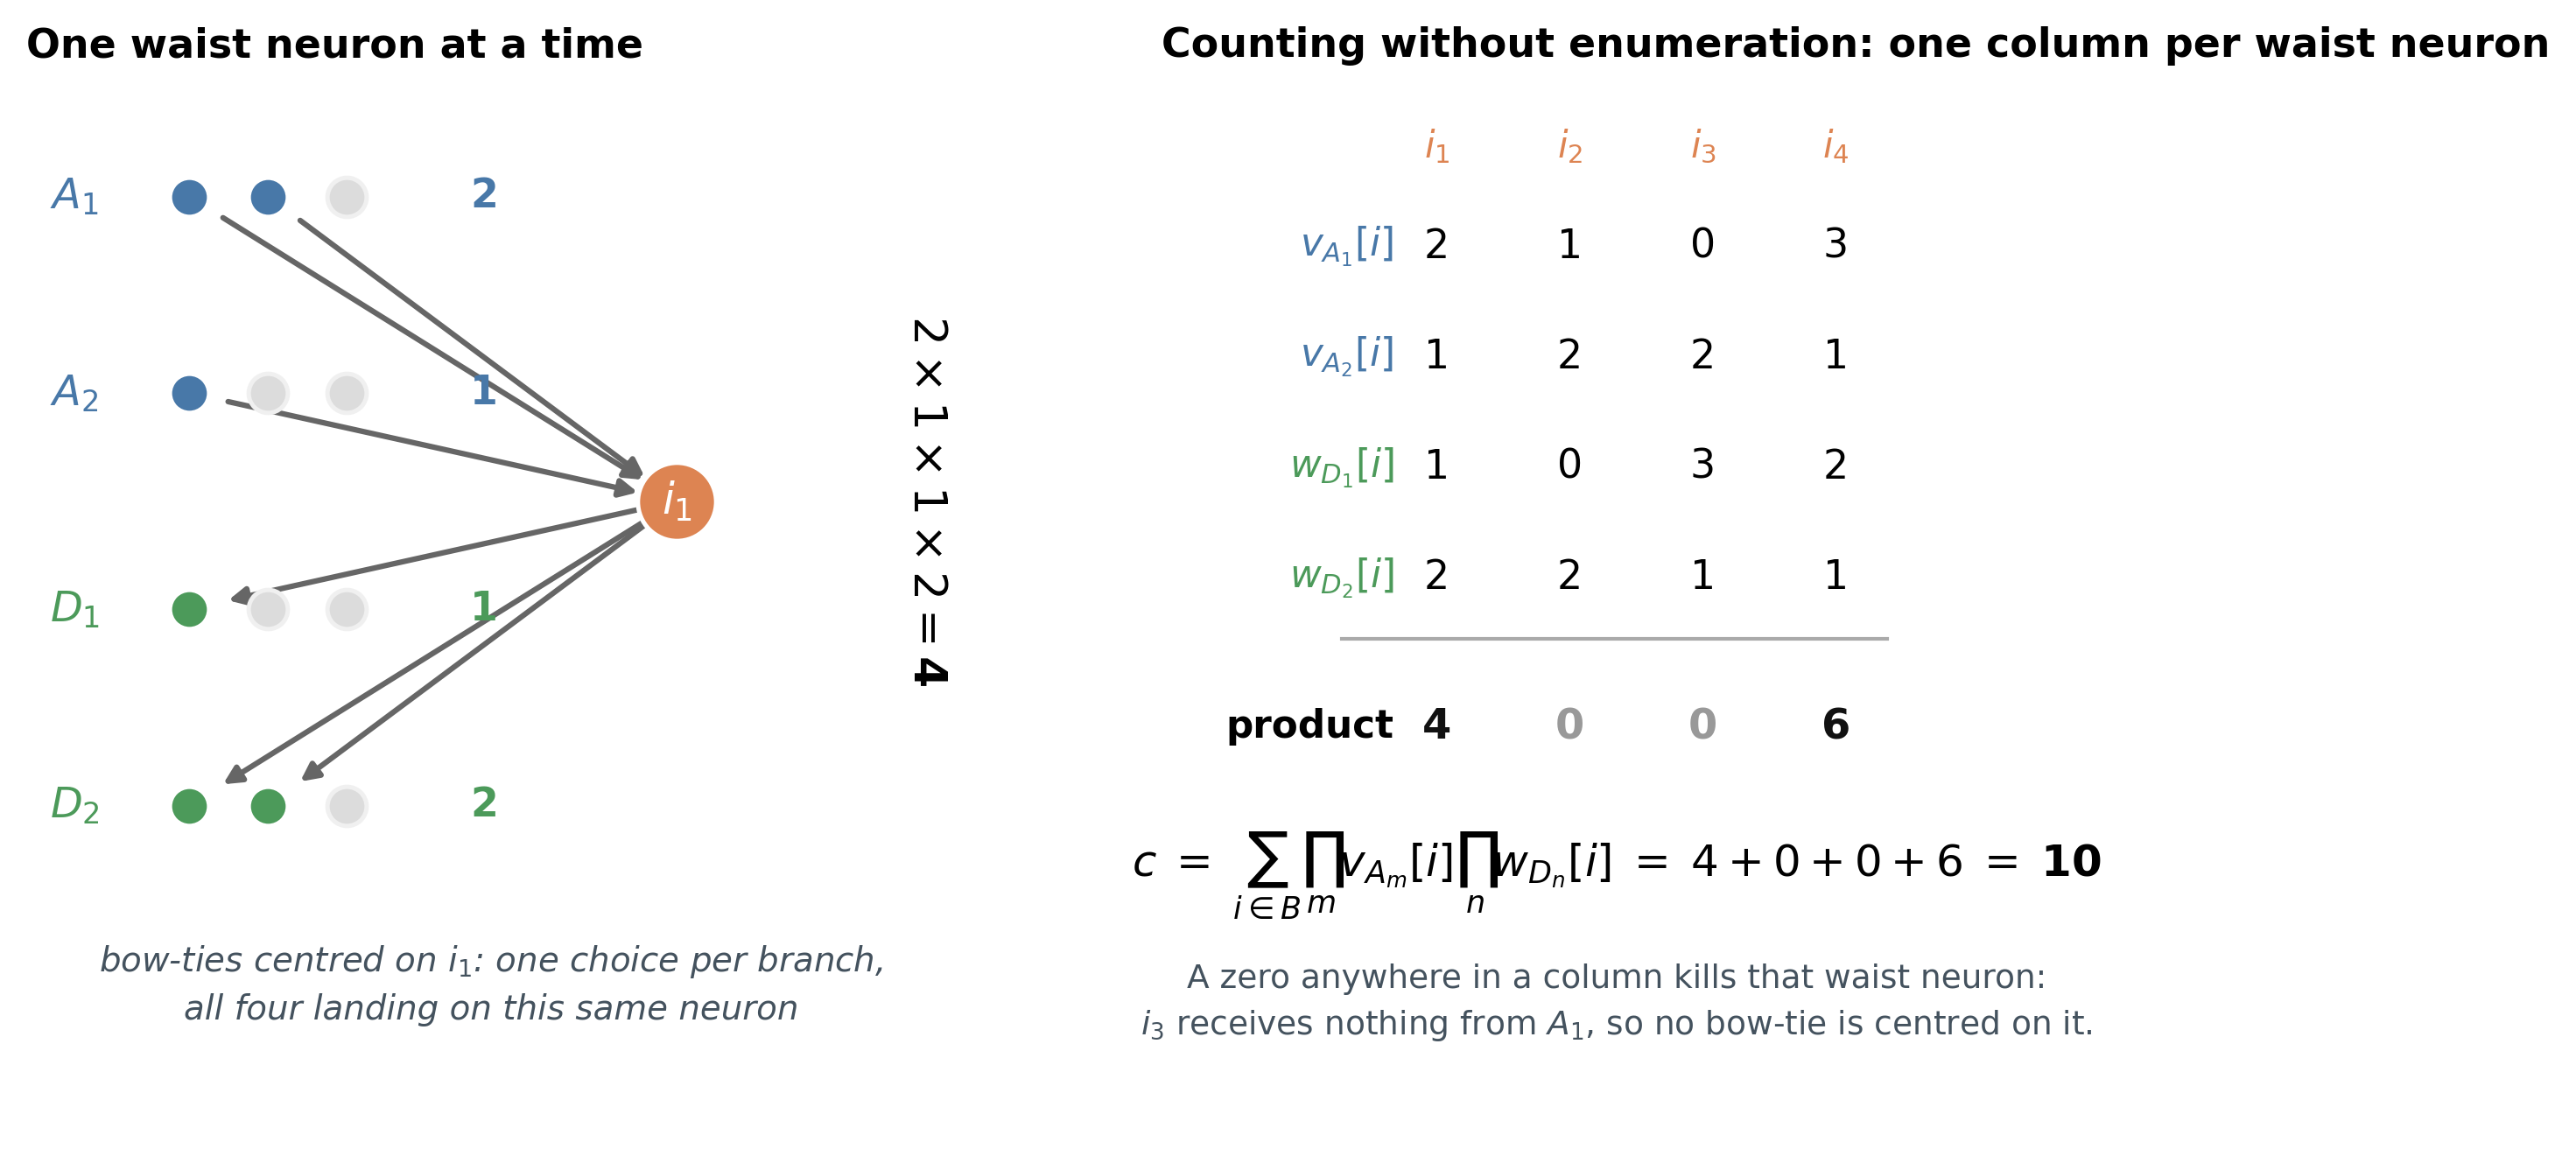
\includegraphics[width=\textwidth]{sigmapi_scheme.png}
\caption[How the bow-tie count factorises]{How the count of a bow-tie
factorises over the waist. On the left, a single waist neuron $i_1$, with the
neurons of each group that actually connect to it drawn in colour and the
rest greyed out: two neurons of $A_1$ project onto it, one of $A_2$, and it
projects onto one neuron of $D_1$ and two of $D_2$, so
$2 \times 1 \times 1 \times 2 = 4$ distinct bow-ties are centred on this
neuron. On the right, the same four counts for every neuron of the waist,
their products, and the sum that gives the count of the pattern. Nothing in
the procedure builds an individual bow-tie.}
\label{fig:sigmapi}
\end{figure}

\subsubsection{The Algebra of Patterns}
\label{sec:pattern-algebra}

The contrast between Equations~\eqref{eq:path-count}
and~\eqref{eq:sigmapi} is not an accident of the bow-tie. It generalises to
a statement about pattern shapes.

\begin{proposition}[Counting cost by pattern shape]
\label{prop:algebra}
Let $P$ be a connectivity pattern to be counted in a graph on $n$ nodes.
If $P$ is a \emph{path}, its count is a pure matrix product, computable in
$O(n)$ memory, and the count is additive over unions of node groups.
If $P$ is a \emph{tree}, its count requires matrix--vector products along
the edges together with an element-wise product at each branching node;
memory remains $O(n)$, but additivity fails at the branching nodes.
If $P$ is \emph{cyclic}, its count is not factorisable over vectors at all,
and a matrix must be maintained, requiring $O(n^2)$ memory.
\end{proposition}

Figure~\ref{fig:pattern-algebra} puts the three cases side by side.

\begin{figure}[H]
\centering
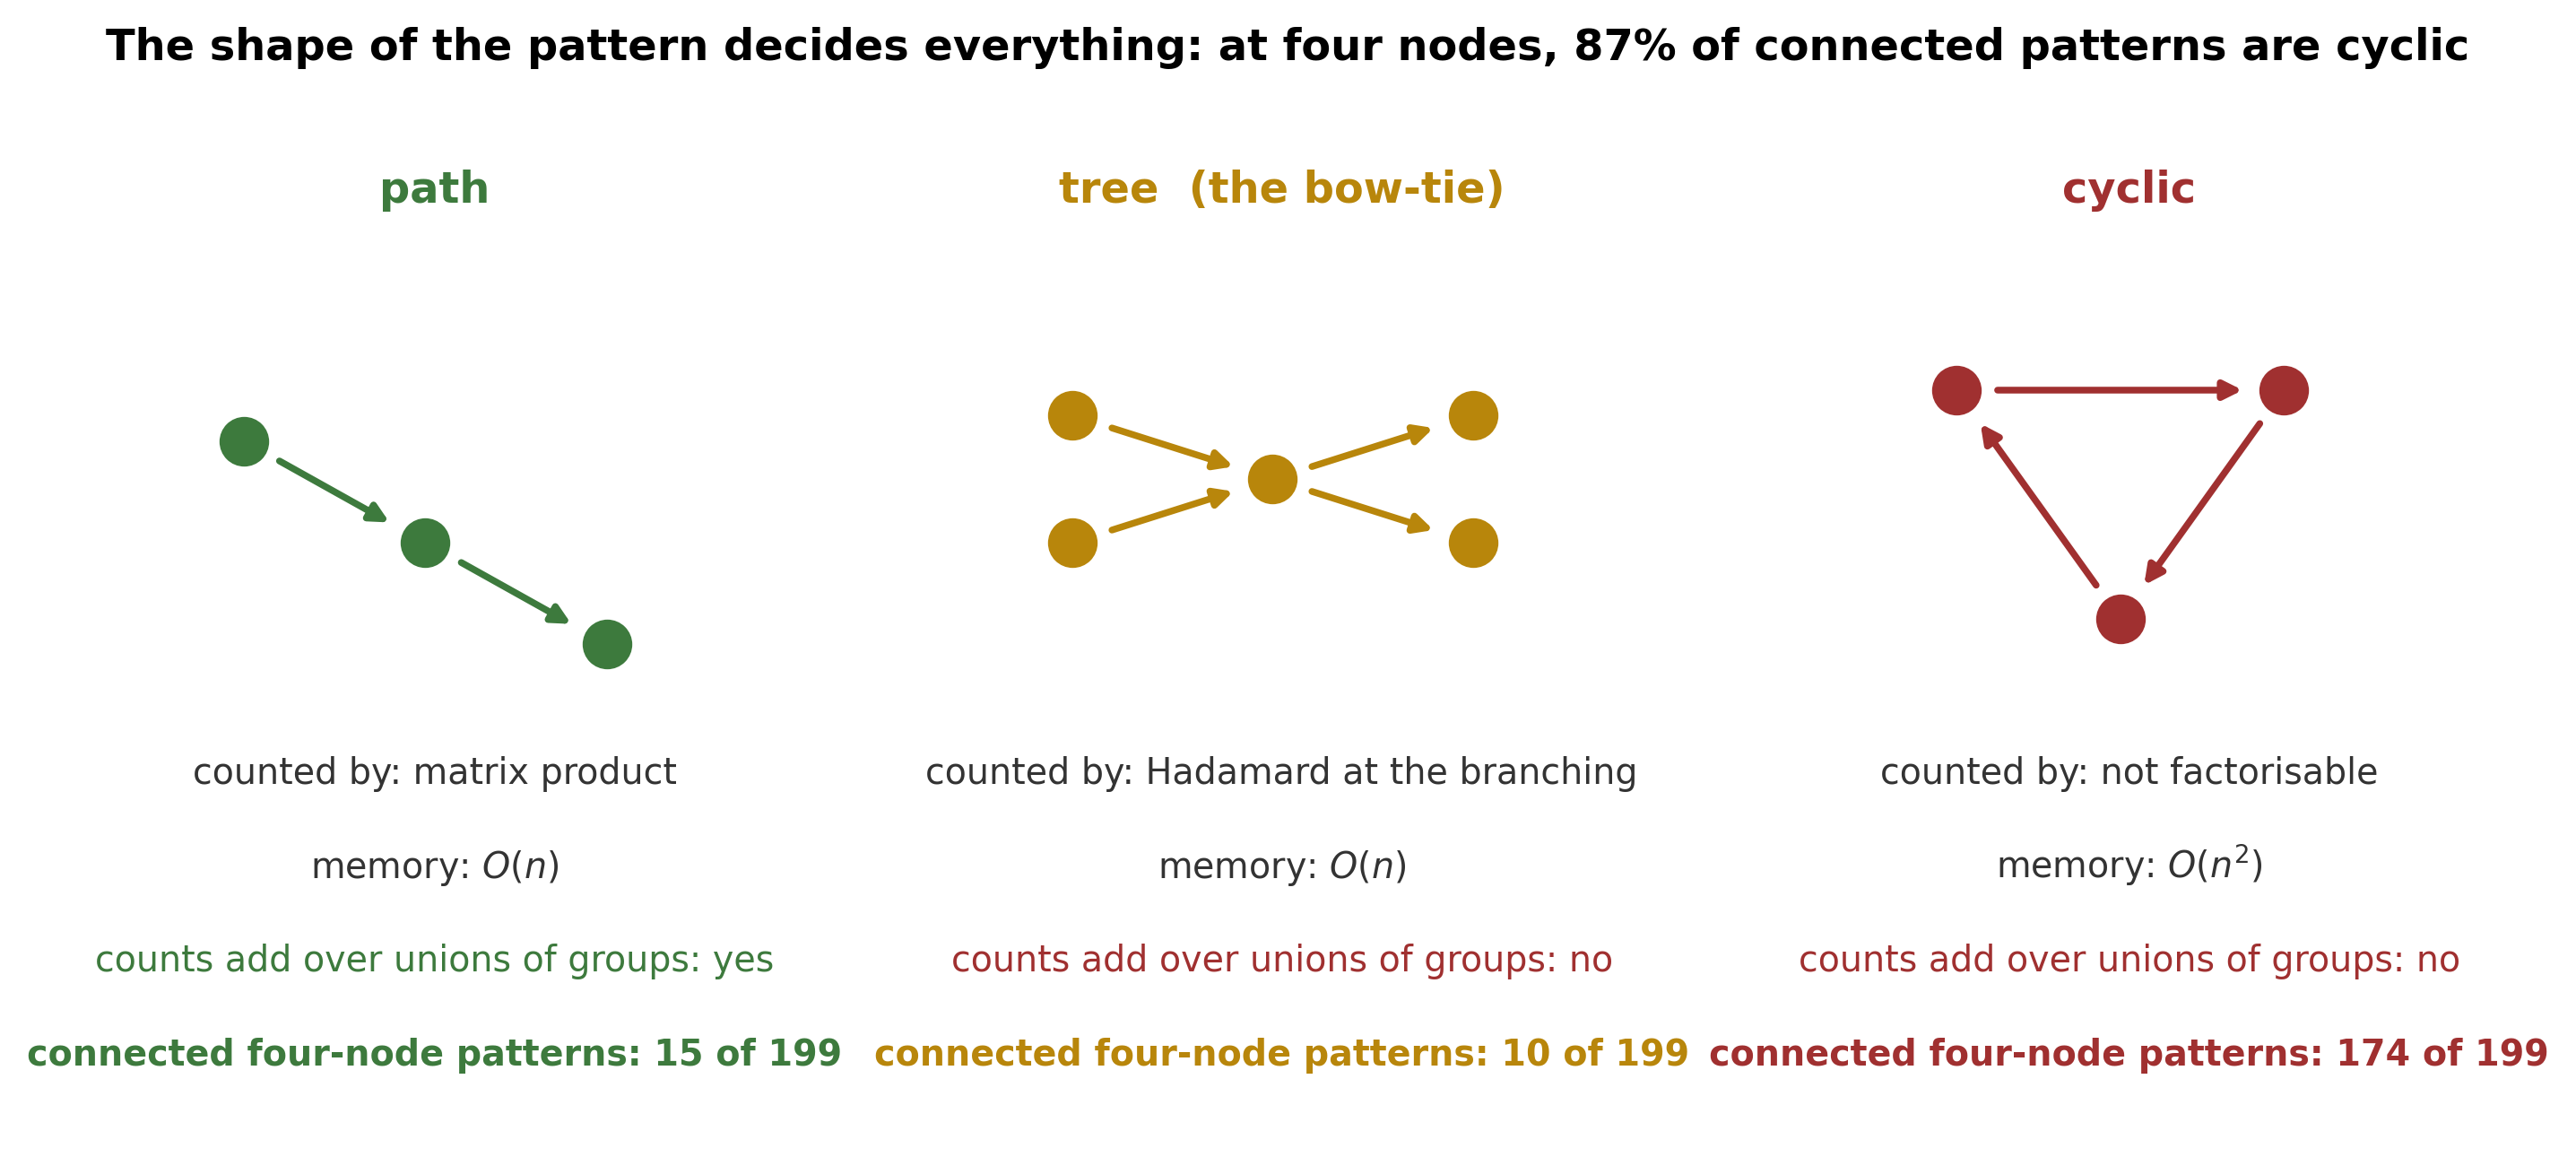
\includegraphics[width=\textwidth]{pattern_algebra.png}
\caption[The three classes of pattern]{The three classes of
Proposition~\ref{prop:algebra}, with what each costs to count. A path is a
chain with no branching: its count is a matrix product and, being linear, it
adds across unions of groups. A tree branches but contains no cycle: the
branching forces an element-wise product, which keeps the memory linear but
destroys additivity, and the bow-tie of this thesis is exactly such a case.
A cyclic pattern admits no factorisation over vectors at all. The counts
beneath each panel are the connected four-node patterns of each kind, from
Table~\ref{tab:pattern-catalogue}.}
\label{fig:pattern-algebra}
\end{figure}

The practical consequence is that the boundary between the cheap and the
expensive is exactly the presence of branching, and that a second boundary,
between the feasible and the infeasible at connectome scale, is the presence
of a cycle. This is not an empirical observation but a consequence of the
structure of the pattern, and it was verified rather than assumed: for all
connected patterns up to four nodes, the closed-form counts derived
automatically from the pattern were compared against explicit enumeration on
random graphs and agreed exactly in every case.

Proposition~\ref{prop:algebra} also answers a question that arises naturally
when one tries to combine circuits. Given the counts of two linear chains
that share a middle node, when is the count of their combination obtained by
composing them? The answer is that composition works along the chain and
fails at the junction, and the junction is precisely where \sigmapi{}
becomes necessary.

\subsubsection{Pragmatic Proof}
\label{sec:algebra-coverage}

Proposition~\ref{prop:algebra} classifies patterns, but it does not by
itself say how much of the space of patterns each class occupies, and
without that the classification could be a distinction without practical
consequence. To settle the question we enumerated all connected
non-isomorphic patterns up to four nodes, derived the factorised counting
formula automatically for each of them, and verified every formula against
exhaustive homomorphism enumeration on random graphs.

\begin{table}[H]
\centering
\caption{Exhaustive catalogue of connected patterns by shape, with formulae
verified against explicit enumeration.}
\label{tab:pattern-catalogue}
\begin{tabular}{rrrrrl}
\toprule
Nodes & Patterns & Paths & Trees & Cyclic & Formulae verified \\
\midrule
3 &  13 &  6 &  0 &   7 (54\%) &  6/6 \\
4 & 199 & 15 & 10 & 174 (87\%) & 25/25 \\
\bottomrule
\end{tabular}
\end{table}

All thirty-one derived formulae reproduced the enumerated counts exactly,
which establishes that the automatic derivation is correct on every case it
was tested against. The figure worth carrying forward, however, is in the
penultimate column of the second row: already at four nodes, $87\%$ of
connected patterns are cyclic and therefore not factorisable over vectors.
The flow-vector and \sigmapi{} machinery is thus powerful on the patterns it
covers and silent on the large majority of the space. That is exactly why a
bow-tie, which is a tree, is a tractable target at connectome scale while a
general motif census is not, and it places the present method in relation to
enumeration-based approaches rather than in competition with them.

Two boundaries of this result should be stated plainly. The catalogue stops
at four nodes because exhaustive enumeration on five would require $2^{20}$
edge masks for $120$ permutations, which this approach cannot reach; the
classification itself does not depend on pattern size, so the qualitative
conclusion carries, but the percentages beyond four nodes are not measured
here. Furthermore, the classification concerns homomorphisms, whereas the
requirement that the participating neurons all be distinct is a separate
layer sitting on top of the count, handled by \emph{inclusion--exclusion}:
one counts without the restriction, then subtracts the cases in which two
nodes coincide, then adds back those subtracted twice, and so on. The two should
not be conflated: factorisability is a property of the shape of the pattern,
whereas node distinctness is a property of the kind of count one wishes to
perform.

\subsection{Macro-Scale Analysis: the \texorpdfstring{$\tau$}{tau}-Core}
\label{sec:macro-methods}

The bow-tie search of the previous section asks a local question: which
groups of neurons form convergent--divergent patterns, and how often. It
cannot, by construction, answer the global one. A network can be full of
local bow-ties without being an hourglass overall, if each of those bow-ties
routes a different part of the traffic and none of them is on the path of
everything else; and conversely a network could funnel all of its traffic
through a handful of neurons that never appear in any frequent local
pattern. The two questions are independent, and the second is the one the
architecture literature actually asks.

This section describes how it is answered. The idea, taken from Sabrin and
Dovrolis \cite{sabrin2020}, is to stop looking at patterns and start looking
at \emph{paths}. If the network really is an hourglass, then a small set of
nodes must lie on almost all the routes from the sensory periphery to the
motor output, and removing that set must disconnect almost everything.
Measuring how small that set is, and comparing it against how small it would
have to be in a network with the same inputs and outputs but no intermediate
structure at all, gives a single number for how hourglass-like the
architecture is. Three definitions are needed to make this precise: the
centrality of a node with respect to paths, the minimal set that covers a
given fraction of them, and the reference against which its size is judged.

\subsubsection{Path Centrality and the \texorpdfstring{$\tau$}{tau}-Core}
\label{sec:taucore-def}

Fix a set of sources $S$ and a set of targets $T$, and let $\Pi$ be the set
of paths from some source to some target. The \emph{path centrality} of a
node $v$ is the number of those paths that pass through it,
\begin{equation}
  \label{eq:path-centrality}
  P(v) = \bigl| \{\pi \in \Pi : v \in \pi\} \bigr|.
\end{equation}
This is computed without enumerating any path. Writing $a_h(v)$ for the
number of paths of exactly $h$ hops from a source to $v$, and $b_h(v)$ for
the number of $h$-hop paths from $v$ to a target, both obtained by
propagating along the layers of the routing, the centrality of $v$ under a
bound $H$ on path length is
\begin{equation}
  \label{eq:centrality-factorised}
  P(v) = \sum_{h_1 + h_2 \le H} a_{h_1}(v)\, b_{h_2}(v),
\end{equation}
which is the same factorisation over a meeting point that
Equation~\eqref{eq:sigmapi} uses for the waist of a bow-tie. The macro and
micro analyses therefore rest on the same algebra, applied once to a pattern
and once to a whole network.

For a set of nodes $X$, let $\pi(X)$ denote the fraction of paths in $\Pi$
that pass through at least one member of $X$. The \emph{$\tau$-core} is the
smallest set covering a fraction $\tau$ of all paths,
\begin{equation}
  \label{eq:taucore}
  C(\tau) = \operatorname*{arg\,min}_{X \subseteq V} |X|
  \quad \text{subject to} \quad \pi(X) \ge \tau .
\end{equation}
Finding the smallest such set exactly is an instance of \emph{set cover},
the problem of choosing the fewest sets that between them cover everything,
which is NP-hard: no algorithm is known that solves it exactly in time
polynomial in the size of the input, and at this scale an exact search is
out of the question. The core is therefore built greedily, as in the
original work: at each step the node of highest
path centrality is added to the core and its paths are removed, and the
centralities are recomputed on what remains. Throughout this thesis
$\tau = 0.9$, so the core is the smallest set of neurons that carries nine
tenths of the sensory-to-motor traffic.

\subsubsection{The Flat Reference and the Hourglass Score}
\label{sec:hscore-def}

The size of $C(\tau)$ is not interpretable on its own, because it depends on
how many sources and targets the network has. A network with ten thousand
sensory neurons will need a large core simply to touch all of them, hourglass
or not. What is needed is a reference: how large would the core have to be in
a network that has the same sources, the same targets and the same
source-to-target dependencies, but no intermediate structure through which to
share them?

That reference is the \emph{flat dependency network} $G_f$, which retains
only the sources and the targets and joins each pair $(s,t)$ by a single edge
whenever a path from $s$ to $t$ exists in the original network. Every path in
$G_f$ has length one, so no node can ever lie on the route of another pair,
and covering a fraction $\tau$ of the dependencies requires naming the
sources and targets themselves. Writing $C_f(\tau)$ for the core of the flat
network, computed by the same greedy procedure, the \emph{hourglass score} is
\begin{equation}
  \label{eq:hscore}
  H = 1 - \frac{|C(\tau)|}{|C_f(\tau)|}, \qquad H \in [0, 1).
\end{equation}
The interpretation follows directly from the definition. If the network
routes its traffic through a narrow waist, then $|C(\tau)|$ is far smaller
than $|C_f(\tau)|$ and $H$ approaches one. If it has no shared intermediate
structure, the two cores are of comparable size and $H$ approaches zero. The
score therefore measures not whether a network has a bottleneck in absolute
terms, but how much narrower its bottleneck is than the flat network its own
inputs and outputs would force. Figure~\ref{fig:flat-reference} shows the
comparison on a sketch small enough to check by eye.

\begin{figure}[H]
\centering
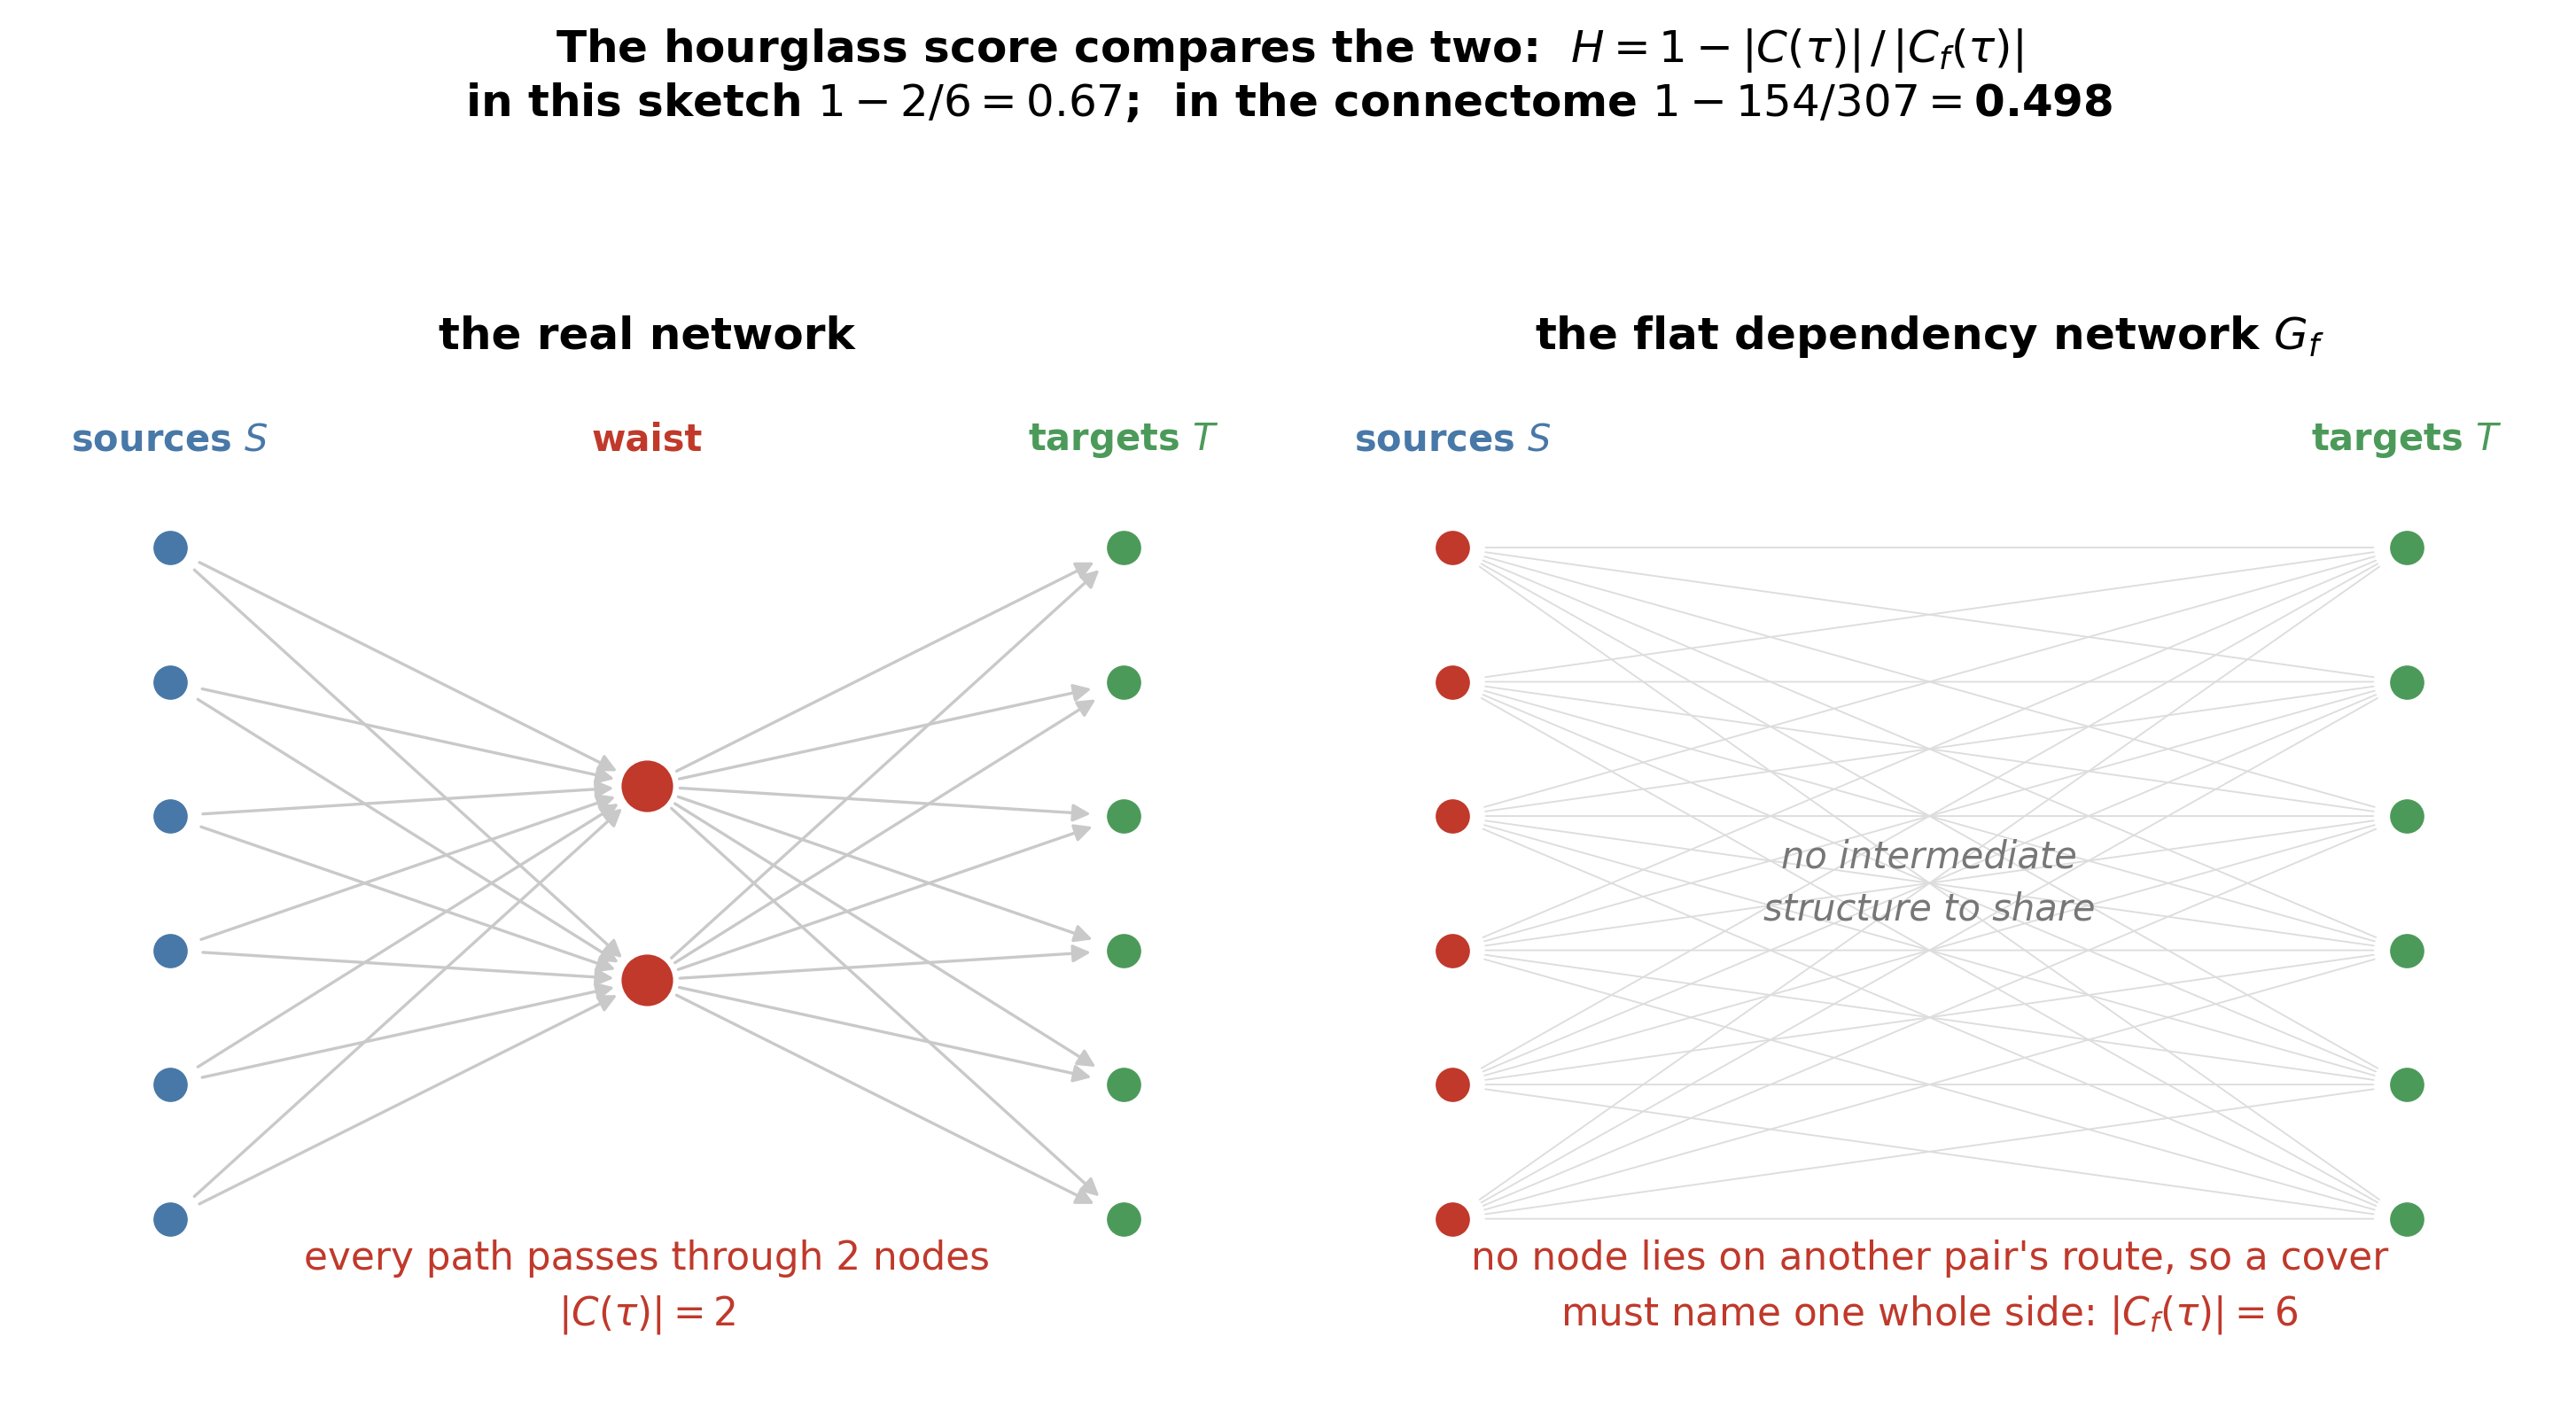
\includegraphics[width=\textwidth]{flat_reference.png}
\caption[The flat reference and the hourglass score]{Why the size of the
core has to be judged against a reference. On the left, a network in which
every route from a source to a target passes through one of two intermediate
nodes: naming those two covers everything, so the core has size two. On the
right, the flat dependency network built from the same sources and targets,
in which each dependent pair is joined directly. No node there lies on any
other pair's route, so covering the dependencies requires naming an entire
side, six nodes. The hourglass score is one minus the ratio of the two, and
it is large exactly when the real network shares intermediate structure that
the flat one cannot.}
\label{fig:flat-reference}
\end{figure}

\subsubsection{Sources, Targets and Routing}

The sources $S$ are taken to be the sensory neurons, of which there are
$12{,}711$, and the targets $T$ the motor and descending neurons, of which
there are $1{,}382$. Computing path centrality then requires a decision
about which paths are to be counted, and this decision matters more than it
might appear.

Two routing schemes are used. Under \code{levels} routing, a path may only
traverse edges that do not decrease the hierarchical level. This makes the
routing acyclic by construction, so that path counts are finite without any
further restriction, at the cost of discarding every lateral edge; because
the acyclicity comes from the structure of the hierarchy itself rather than
from an imposed bound, this scheme is referred to as \emph{structural
routing} wherever the results are discussed. Under \code{score} routing, paths follow a
continuous flow score which recovers part of the lateral connectivity, with
an explicit bound imposed on the length of admissible paths. Since almost
$39\%$ of all edges in this connectome are lateral, the difference between
the two
schemes is substantial and both are reported throughout.

\subsubsection{Why the Path Length Bound Is Mandatory}

The bound $H$ on path length in Equation~\eqref{eq:centrality-factorised}
was introduced without comment, and it deserves one, because it is not a
computational convenience but a condition for the centrality to be defined
at all.

In a cyclic graph the number of source-to-target paths diverges
combinatorially with the permitted path length, since paths may wander
through cycles arbitrarily many times. As the count diverges, the ordering
of nodes by path centrality degenerates, because a single well-connected
neuron appears on an overwhelming proportion of the increasingly baroque
paths. Section~\ref{sec:results-macro} quantifies exactly how bad this
becomes. The bound on path length is therefore not a computational
convenience that could be relaxed given more resources, but a definitional
requirement without which the measure has no content.

\subsection{Micro-Scale Analysis: Bow-Tie Motif Search}
\label{sec:micro-methods}


Where the previous section asked whether the network as a whole funnels its
traffic, this one asks which structures do the funnelling. The object counted
is the bow-tie of Definition~\ref{def:bowtie}, over metanodes rather than
neurons, and the counting uses the \sigmapi{} formulation of
Section~\ref{sec:sigmapi} directly.

Three things have to be settled before a search can be run: which
configurations are admissible, how the space of candidates is cut down
enough to make an exhaustive pass feasible, and how the resulting waists are
compared with one another. This section takes them in that order.

\subsubsection{Search Space and Parameters}

The search is governed by four parameters. The level window $NL$ fixes the
set of hierarchical levels within which motifs are sought, so that
$NL = \{1,2,3\}$ restricts attention to early sensory processing while
$NL = \{3,4,5\}$ examines deep integration. The parameters $\kin$ and
$\kout$ set the number of input and output groups of the bow-tie. The
parameter $\mathit{max\_jump}$ bounds the level difference that a single
edge of the metagraph may span, and setting it to one imposes a
layer-by-layer processing logic in which a connection may move at most one
level up or down. Finally $\mathit{min\_count}$ sets the minimum number of
occurrences a pattern must have to be retained, which suppresses the long
tail of patterns realised by only a handful of neurons. Unless stated
otherwise, all results in this thesis use $\kin = \kout = 2$,
$\mathit{max\_jump} = 1$ and $\mathit{min\_count} = 10$.

The choice $\kin = \kout = 2$ deserves a word, since the framework imposes no
such restriction. It is the smallest configuration that is genuinely a
bow-tie: two inputs are the minimum needed for convergence and two outputs
the minimum for divergence, whereas $\kin = \kout = 1$ describes a linear
chain rather than a waist, and linear chains through this hierarchy have
already been characterised in earlier work on the same dataset
\cite{curcio2026}. Taking the smallest structure that expresses the
architecture under study also keeps the count interpretable, since every
pattern is then a statement about four edges rather than about an
increasingly baroque configuration.

The framework is nonetheless parametric in both values, and the search engine
accepts any $\kin$ and $\kout$: configurations such as $(3,3)$ and $(3,2)$
run without modification. What makes larger values impractical is cost rather
than expressiveness. The number of group combinations per waist grows as
$\binom{p}{\kin}\binom{q}{\kout}$, so a waist with fifty incoming and fifty
outgoing groups goes from $1.5$ million combinations at $\kin=\kout=2$ to
$384$ million at three, a factor of $256$; interpretation degrades in the
same direction, since each pattern then constrains six edges rather than
four.

A genuine implementation limit applies only to the parameter sweep of
Section~\ref{sec:results-sweep}. That sweep avoids enumerating combinations
by evaluating an \emph{elementary symmetric polynomial}: given a list of
numbers, the $k$-th such polynomial is the sum of all products of $k$ of
them taken at a time, which is exactly the quantity a sum over all
$k$-combinations of groups requires, and which can be computed without
forming a single combination. That shortcut admits an exact
disjointness correction only for the pure forms $(k,1)$ and $(1,k)$; the
general case $(k,k)$ with $k \ge 3$ would require inclusion--exclusion to a
depth this implementation does not reach.

\subsubsection{Pruning}
\label{sec:pruning}

Three constraints reduce the search space, and it is important that none of
them affects exactness: each removes only combinations that provably
contribute nothing. The first is the disjointness requirement of
Definition~\ref{def:bowtie}, which excludes combinations in which an input
group also appears among the outputs. The second is a restriction to the
support of the waist: only those waist neurons that are reachable from at
least one input group and that in turn reach at least one output group can
possibly contribute to a count, so all others are removed before any product
is formed. The third is an early exit on null flow, which discards any
combination in which one of the factors of Equation~\eqref{eq:sigmapi} is
identically zero, since the product is then zero regardless of the remaining
factors. On the shallow window these three together eliminate more than
$97\%$ of the nominal search space.

\subsubsection{Compression Metrics}
\label{sec:compression-methods}

A waist is interesting to the extent that it \emph{compresses}, that is, to
the extent that many peripheral neurons are routed through few central ones.
The obvious way to measure this is to take the ratio of the number of
peripheral neurons to the size of the waist group, but that measure fails in
practice, and understanding why it fails motivates the correct one.

The difficulty is that a group may be nominally large while only a handful
of its neurons actually participate in any given pattern. A waist of twenty
neurons of which two carry all the flow behaves, functionally, like a waist
of two, and dividing by twenty understates its compression by an order of
magnitude; conversely, a group of twenty neurons that all participate
equally is a genuinely distributed bottleneck. What is needed is a measure
of the \emph{effective} number of participating neurons, one that equals the
group size when all neurons contribute equally and falls towards one when a
single neuron dominates.

The participation ratio provides exactly that. Writing $P_i$ for the
\sigmapi{} contribution of waist neuron $i$, that is, the number of bow-ties
centred on that neuron, we define
\begin{equation}
  \label{eq:neff}
  \neff = \frac{\left(\sum_i P_i\right)^2}{\sum_i P_i^2},
  \qquad
  \text{realised compression} =
  \frac{\text{peripheral neurons connected to an active waist}}{\neff}.
\end{equation}
If $k$ neurons contribute equally and the rest not at all, the numerator is
$(kP)^2$ and the denominator $kP^2$, so that $\neff = k$ as required. If one
neuron carries everything, both sums are dominated by that neuron and
$\neff$ tends to one. Section~\ref{sec:results-compression} shows what
difference the correction makes to the ranking of waists in practice.

\subsection{Statistical Validation}
\label{sec:validation-methods}


A pattern that occurs frequently is not thereby a motif. Large networks
contain enormous numbers of every small pattern simply because they are
large and because some neurons have very many connections, and a count on
its own cannot distinguish structure from that background. The comparison
against randomised networks is therefore not a check applied at the end but
part of what the word motif means, as Section~\ref{sec:motifs} noted.

The difficulty is that there is no single correct randomisation. Each choice
of what to preserve and what to destroy tests a different explanation, and a
pattern can be significant against one and unremarkable against another; this
thesis reports a case where the ordering of patterns inverts between two of
them. Three null models are therefore used rather than one, and this section
describes them, the way significance is assessed given the shape of the
resulting distributions, and how the size of an effect is reported once
significance is established.

\subsubsection{Three Complementary Null Models}

A single null model tests a single confound, and can therefore only ever
establish that the observed structure is not explained by that one thing.
Because several different properties of the connectome could plausibly
generate an apparent excess of bow-ties, we use three null models, each of
which destroys a different aspect of the observed structure while preserving
the others.

The three are the following.

\begin{itemize}
  \item \textbf{Model A, degree-preserving.} The classical null of Milo et
    al.\ \cite{milo2002,maslov2002}. The network is rewired through repeated
    edge swaps that leave the in-degree and out-degree of every neuron
    unchanged. It preserves the degree sequences exactly and destroys the
    anatomy completely, so a pattern still over-represented under it cannot
    be explained by degree alone.

  \item \textbf{Model B, block-density-preserving.} Edges are resampled
    independently within each pair of anatomical groups, at the density
    observed for that pair. It preserves how strongly any two regions are
    connected and destroys individual degrees, so it tests whether a pattern
    is explained by regional connectivity alone.

  \item \textbf{Model C, degree permutation within blocks.} The strictest of
    the three. Within each block the assignment of degrees to individual
    neurons is permuted, preserving both the number of edges and the
    per-block degree sequences, and randomising only \emph{which} waist
    neuron receives which degree. It leaves everything intact except the
    coincidence structure at the waist, which is precisely the property a
    bow-tie count depends on.
\end{itemize}

The three are therefore nested in strictness rather than alternative to one
another, and a pattern that survives all three has been shown not to follow
from degree, from regional density, or from the way degree is distributed
within a region. Figure~\ref{fig:null-models} shows what each one does to a
small network.

\begin{figure}[H]
\centering
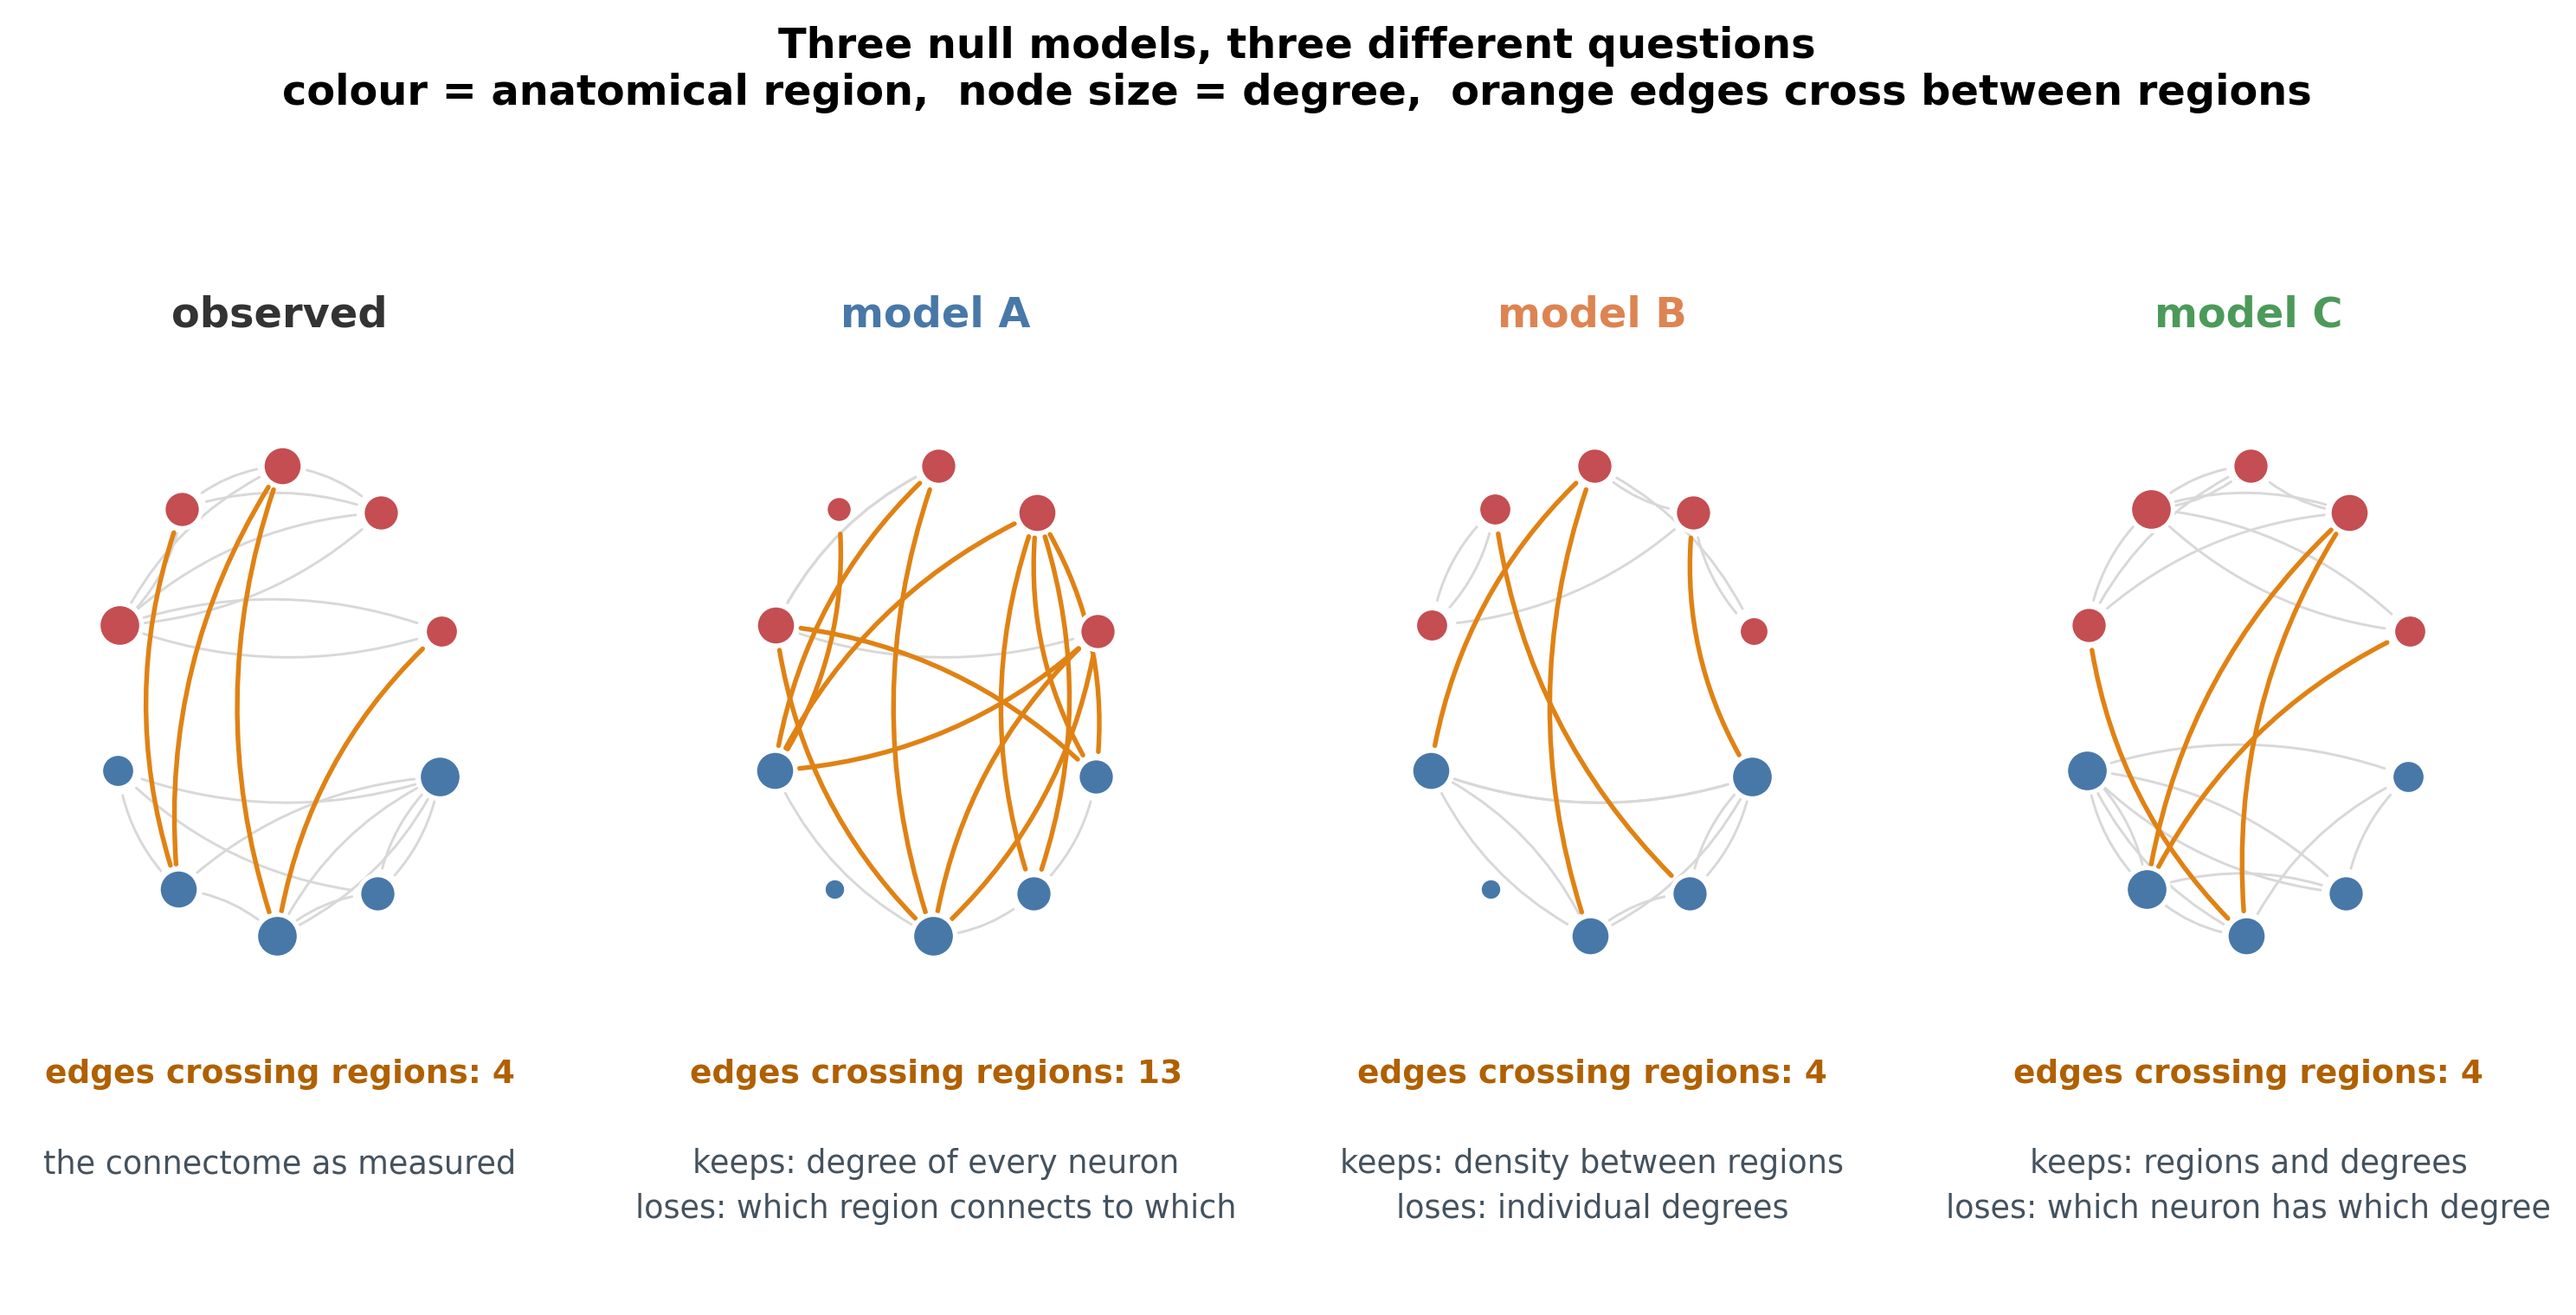
\includegraphics[width=\textwidth]{null_models.png}
\caption[What each null model preserves and destroys]{The three null models
applied to the same small network, whose ten nodes belong to two anatomical
regions shown in two colours. The size of a node is its degree and the edges
that run between the two regions are drawn in orange, so the two properties
each model is concerned with are both visible. Model A keeps every degree
but scatters the edges across regions, and the count of crossing edges rises
sharply. Model B keeps the number of crossings and randomises the degrees.
Model C keeps both and permutes only which node within a region carries
which degree, which is why it is the strictest of the three: what it
randomises is precisely the coincidence structure a bow-tie count depends
on.}
\label{fig:null-models}
\end{figure}

\subsubsection{Inference}

Significance is assessed with empirical $p$-values,
\begin{equation}
  \label{eq:pvalue}
  p = \frac{1 + \#\{c_{\mathrm{rand}} \ge c_{\mathrm{real}}\}}{N+1},
\end{equation}
where $c_{\mathrm{real}}$ is the observed count and the $c_{\mathrm{rand}}$
are the counts obtained on $N$ randomised networks. We use empirical
$p$-values rather than $z$-scores because the null distribution of motif
counts is strongly right-skewed, so that a $z$-score does not correspond to
a tail probability and would systematically overstate significance.

The set of patterns to be tested is \emph{pre-registered}: it consists of
the twenty most frequent patterns of each of the sixteen signatures, three
hundred and twenty patterns in all, selected before any randomisation was
examined. This matters because selecting patterns after seeing which ones
look unusual would guarantee significance by construction. Multiple testing
across the three hundred and twenty tests is controlled with the
Benjamini--Hochberg false discovery rate procedure \cite{benjamini1995},
which bounds the expected proportion of false positives among the
rejections. Randomisation uses $N = 100$ samples with a fixed seed, and the
mixing of the edge-swap chain was verified empirically rather than assumed
by checking that the results stabilise well before the number of swaps
actually used.

\subsubsection{Effect Size}

The ratio between the real count and the median randomised count is
deliberately \emph{not} reported as an effect size anywhere in this thesis.
It spans several orders of magnitude across the three null models and is
dominated by how thoroughly each model destroys the structure rather than by
any property of the data, which makes it uninterpretable as a measure of
biological strength. Section~\ref{sec:null-inversion} shows that the ratio
does not even preserve the ordering between signatures from one null to
another, which settles the matter.

\subsection{Computational Realisation}
\label{sec:engine}


The formulation of Section~\ref{sec:counting} makes an exhaustive count
possible in principle. Making it possible in practice, on a network of
$134{,}181$ neurons, required three pieces of engineering, and they are
described here because the analysis of the deeper windows would not have
been feasible without them: a reformulation of the inner loop as a matrix
product, a sparse variant for the cases where the dense form does not fit in
memory, and a decision about what to keep of an output that would otherwise
run to hundreds of gigabytes.

\subsubsection{The Matrix Engine}

A direct implementation of Equation~\eqref{eq:sigmapi} loops over
combinations of groups and performs, for each one, a copy followed by
$\kout$ multiplications and as many additions over arrays of the length of
the waist. On the shallow window this amounts to roughly $1.7$ billion
iterations, and profiling shows something initially surprising: the cost is
dominated not by the arithmetic but by the per-call overhead of the array
library, some two microseconds per call. The computation is therefore
limited by how often the inner loop crosses into the numerical library, not
by how much numerical work it does.

The remedy is to arrange for all combinations of a given waist to be
computed at once. Let $P_{\mathrm{in}}$ be the matrix whose row $r$ is the
element-wise product of the input flow vectors of combination $r$, and let
$P_{\mathrm{out}}$ be the analogous matrix for the output combinations. Then
every count belonging to that waist is an entry of
\begin{equation}
  \label{eq:matrix-engine}
  T = P_{\mathrm{in}} P_{\mathrm{out}}^{\top},
\end{equation}
a single dense matrix product which can be delegated wholesale to the
optimised linear algebra library. Billions of individual calls collapse into
a few thousand matrix products.

The compression metrics of Section~\ref{sec:compression-methods} follow the
same pattern and need not be computed separately per combination. Since the
per-combination vector is the element-wise product of an input row and an
output row, the sum of its squares and the count of its non-zero entries are
themselves matrix products,
\begin{equation}
  \textstyle\sum_i p_{v,i}^2 = P_{\mathrm{in}}^{2} (P_{\mathrm{out}}^{2})^{\top},
  \qquad
  n_{\mathrm{active}} = (P_{\mathrm{in}} > 0)(P_{\mathrm{out}} > 0)^{\top},
\end{equation}
so that the vector itself is never materialised for any individual
combination.

\subsubsection{The Sparse Engine}

Equation~\eqref{eq:matrix-engine} requires memory proportional to the number
of combinations multiplied by the size of the waist, and therefore switches
itself off precisely on the largest waists. This is unfortunate, because
those are the expensive ones: on the shallow window the waists that exceed
the memory budget account for the majority of the total runtime.

The way out comes from observing that on a large waist the flow vectors are
almost entirely zero. An input group typically reaches only a few hundred of
the $24{,}835$ neurons of the largest metanode, so the matrices in
Equation~\eqref{eq:matrix-engine} are dense representations of almost
nothing. Computing the same product with sparse operands produces directly,
and only, the pairs whose count is non-zero, and those are exactly the pairs
that need to be emitted. Memory then scales with the number of non-zero
entries rather than with the product of the dimensions, and the constraint
that forced the fallback disappears. The three quantities computed
alongside the count share the same sparsity structure, since the values are
non-negative counts and a product vanishes if and only if one of its factors
does; that this alignment holds is asserted at run time rather than assumed.

\subsubsection{Output Distillation}
\label{sec:distillation}

Exhaustive counting produces one row of output per pattern, and for the full
window that means $512{,}969{,}374$ rows. Retained as plain text these rows
occupy more than $100$\,GB across the four windows, which is unwieldy to
store and slow to read.

Examining what the downstream analyses actually consume shows that none of
them uses the individual rows. Every one of them either aggregates the rows
into summary counts or selects a top-$N$ subset by frequency. The row-level
output is therefore an intermediate rather than a result: it needs to exist
for the duration of a single pass and no longer. The search engine
consequently retains only the aggregates, computed by signature, by waist
and by level chain, together with top-$N$ selections in which the complete
rows are kept. This reduces the four windows from over $100$\,GB to
$68$\,MB while producing downstream results that are identical.

The selections are deliberately wider than any current analysis requires,
and they are stratified by waist and signature jointly as well as by waist
alone, so that comparisons made at parity of waist between classes of motif
remain possible. Section~\ref{sec:results-nt} depends on exactly that
stratification.

\subsection{Correctness Verification}
\label{sec:verification}

Three independent mechanisms are used to establish correctness, and they are
described here in some detail because the credibility of every number in
Section~\ref{sec:results} rests on them.

The first is a reference implementation. A slow but readable implementation
of Equation~\eqref{eq:sigmapi}, written directly from the mathematics
without any of the optimisations, is retained alongside the fast engine. The
two are compared row by row across all $1{,}043{,}872$ rows and all $26$
columns of a complete run, including $24$ waists deliberately forced onto
the sparse path by lowering the memory budget so that the sparse code is
exercised rather than merely present.

The second is exhaustive enumeration. Every closed-form count in this thesis
is checked against explicit enumeration on random graphs where enumeration
is feasible: the within-area formula of
Section~\ref{sec:results-within} on three hundred random graphs, the
symmetric-polynomial formulation used for the $(\kin, \kout)$ sweep, and the
pattern algebra of Proposition~\ref{prop:algebra}. A closed form that agrees
with brute force on small cases can still be wrong on large ones, but a
closed form that disagrees on small cases is certainly wrong, and this check
has caught real errors during development.

The third is internal consistency. Each analysis recomputes the occurrence
count of every pattern it handles directly from the graph and compares it
against the stored value, so that a corrupted or misaligned intermediate
would be detected at the point of use. All such checks reported exact
agreement.

%=======================================================================
\section{Results}
\label{sec:results}

The results follow the same path as the methods: from the whole network
inwards.

They open with the hierarchy on which everything else is conditioned,
establishing what the five levels contain and how densely they are wired,
and then testing whether that hierarchy remains meaningful when neurons are
grouped by anatomy rather than by function. With the axis established, the
global question is asked: does this connectome route its traffic through a
narrow waist, and how does the answer compare with the one obtained for
\textit{C.\ elegans}. The analysis then descends to the local scale, where
the exhaustive motif search across four level windows identifies which
structures actually form those waists, how the picture changes with depth,
and how much the choice of anatomical granularity determines what can be
seen. The two scales are then compared directly against each other.

The remaining sections take up questions that either scale raises on its own:
whether the counts survive randomisation, what the neurochemistry of the
waists is, how the picture changes when the shape of the pattern is allowed
to vary from integrative to broadcast, what happens inside a single
anatomical area, and what the whole analysis costs to run.
%=======================================================================

\subsection{Hierarchical Structure of the Connectome}
\label{sec:results-hierarchy}


Everything that follows is conditioned on the five hierarchical levels, so
the first thing to establish is what they contain and how they are wired to
one another. This section reports the size and functional composition of
each level, the density of connections between them, and the balance of
forward, backward and lateral edges. The last of these turns out to matter
for the macro-scale analysis, which discards a substantial fraction of the
edges depending on how paths are routed.

\subsubsection{Level Sizes and Composition}

Since the level assignment is inherited rather than derived here, the first
thing to establish is that it means what it is supposed to mean.
Table~\ref{tab:levels} reports how the neurons are distributed across the
five levels together with the functional composition of each level, and
Figure~\ref{fig:level-composition} shows the same two quantities.

\begin{table}[H]
\centering
\caption{Neurons per hierarchical level and functional super-class
composition (percentages by row).}
\label{tab:levels}
\begin{tabular}{lrrrrrrr}
\toprule
Level & Neurons & \% & optic & sensory & central & descending & vis.\ proj. \\
\midrule
L1 & 13,601 & 10.1 & 51.7 & \textbf{42.3} & 3.9 & 0.0 & 0.6 \\
L2 & 47,049 & 35.1 & 75.6 & 8.6 & 11.6 & 0.1 & 2.3 \\
L3 & 44,265 & 33.0 & 67.6 & 3.2 & 21.3 & 0.3 & 6.1 \\
L4 & 17,124 & 12.8 & 26.9 & 4.9 & 48.0 & 1.4 & 16.3 \\
L5 & 12,142 &  9.0 &  3.2 & 5.5 & \textbf{71.3} & \textbf{6.9} & 8.3 \\
\bottomrule
\end{tabular}
\end{table}

\begin{figure}[H]
\centering
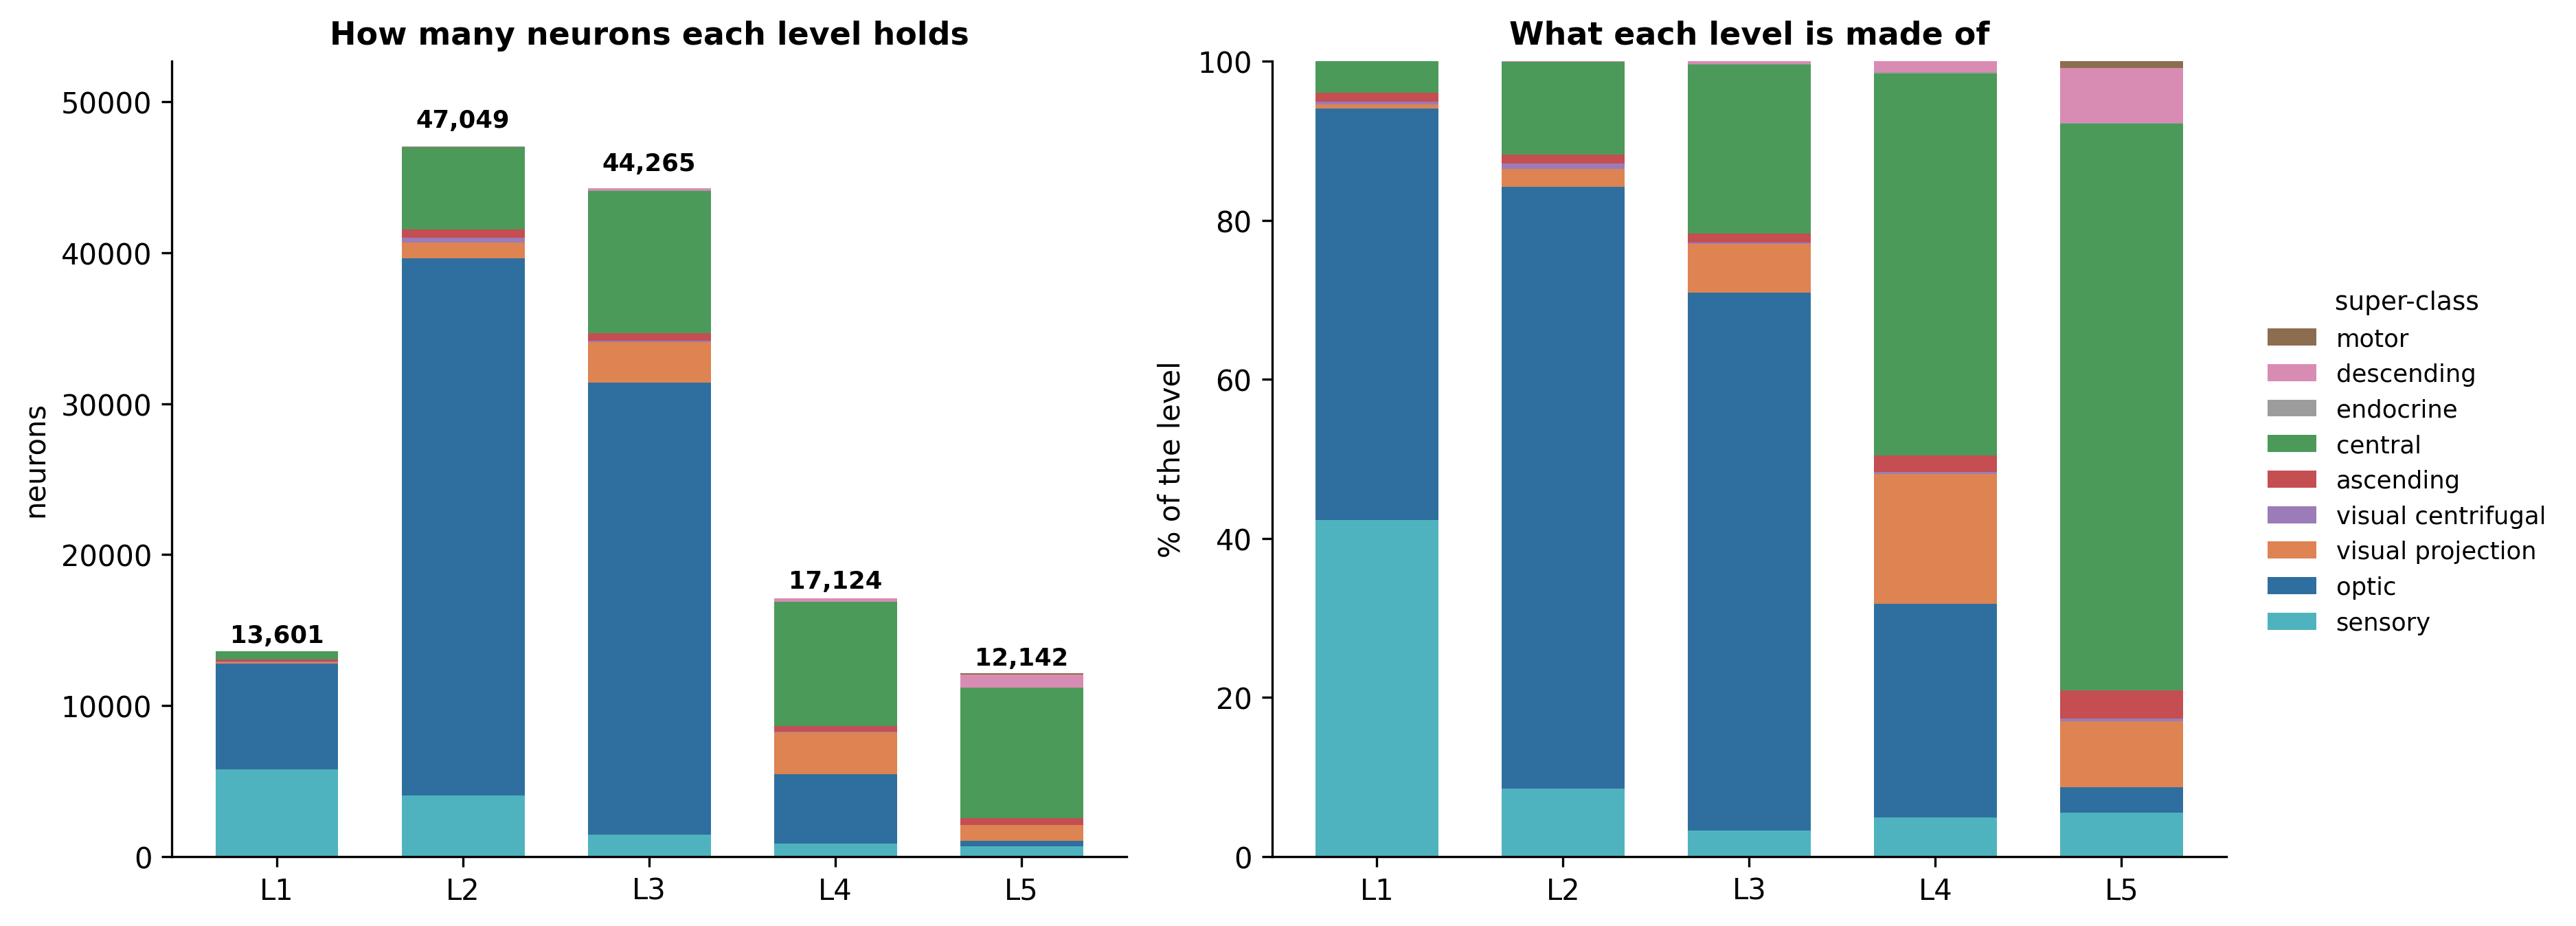
\includegraphics[width=\textwidth]{level_composition.png}
\caption[Level sizes and functional composition]{The five levels by size and
by content. On the left, how many neurons each level holds; on the right, the
same populations normalised, so that the composition can be compared across
levels of very different size. The super-classes are stacked in
sensory-to-motor order, and the resulting picture is a gradient: sensory and
optic neurons fill the shallow levels, central neurons take over from
level~4, and descending neurons, which carry signals out of the brain towards
the motor system, appear in quantity only at level~5.}
\label{fig:level-composition}
\end{figure}

The gradient is monotone in the expected direction. Sensory content falls
from $42.3\%$ at level~1 to $5.5\%$ at level~5, central content rises from
$3.9\%$ to $71.3\%$ over the same range, and descending neurons appear only
at the two deepest levels.

How much this confirms requires care, because the level boundaries were
themselves chosen to separate super-classes, as
Section~\ref{sec:levels} described. Reading the gradient as independent
confirmation of the levels would therefore be circular, and it is not
claimed here. What the gradient does confirm is something else, and it is
worth separating the two.

The construction has two stages, and only the second one saw the super-class
labels. The spectral embedding that produces the flow score is computed from
connectivity alone: it knows which neuron projects to which, and nothing
about what any of them does. The decision tree then chose four numbers on
that one-dimensional axis. Four thresholds are very little freedom, and no
choice of them could have produced the gradient of
Figure~\ref{fig:level-composition} if the underlying axis had not already
ordered the neurons that way. The alignment is therefore evidence about the
\emph{embedding}, not about the discretisation: a quantity derived purely
from wiring turns out to sort neurons into the same order that their
biological function does. That is a genuine result, and it is the reason the
levels can be trusted as an axis of information flow. What it is not is a
validation of where exactly the four cuts fall, which remains a modelling
choice inherited from earlier work.

\subsubsection{Connection Density}

Raw counts of edges between levels are dominated by the sizes of the levels
involved: level~2 alone contains $47{,}049$ neurons, so any transition
touching it appears large simply on that account. The informative quantity
is therefore the density, defined as the number of edges observed per ten
thousand pairs of neurons that could possibly be connected.
Figure~\ref{fig:level-density} shows the full matrix.

\begin{figure}[H]
\centering
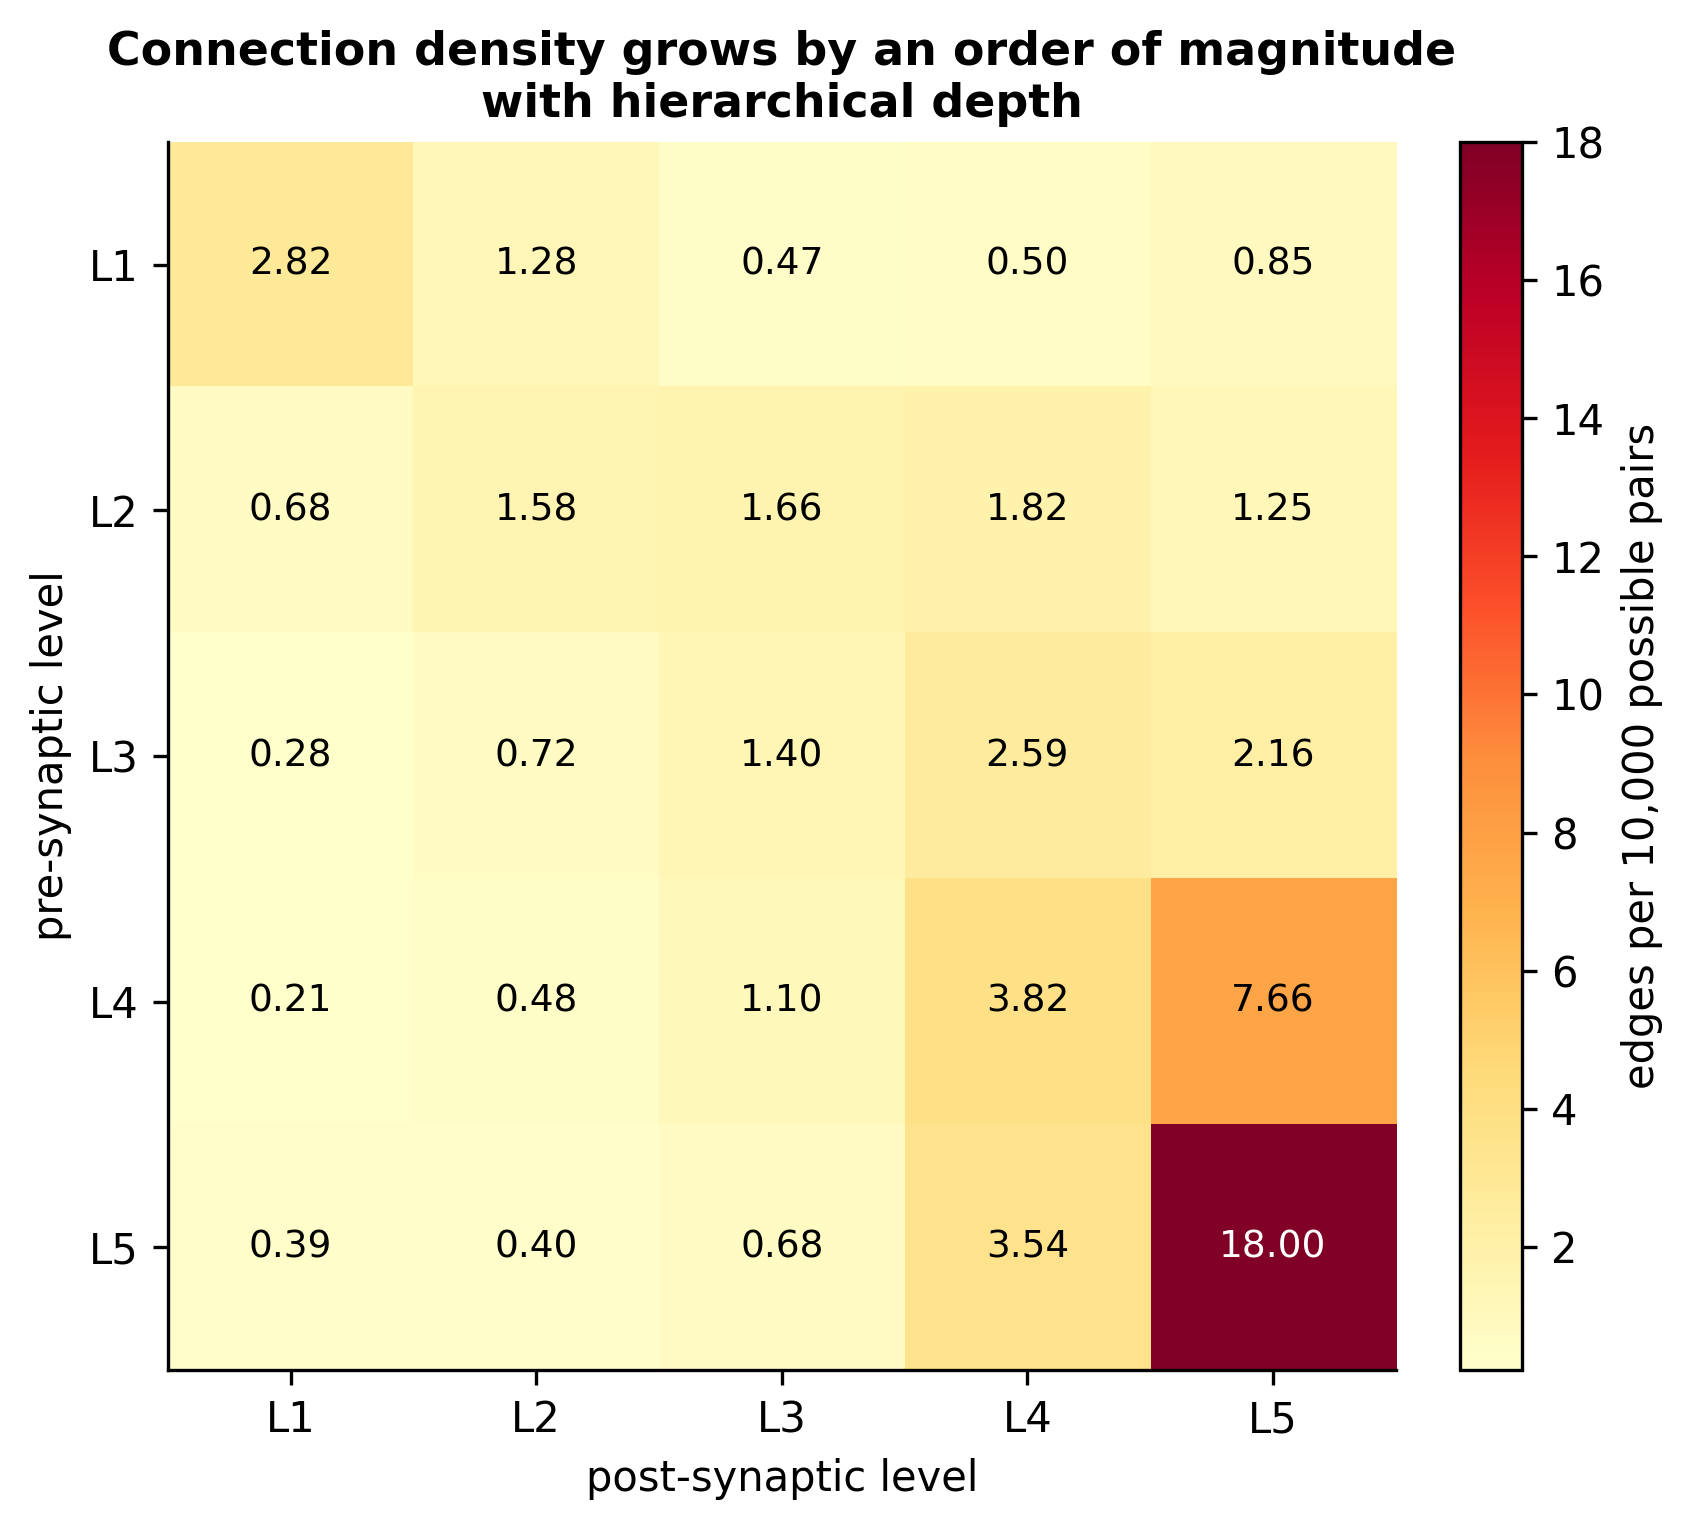
\includegraphics[width=0.68\textwidth]{level_density.png}
\caption[Level-to-level connection density]{Connection density between
hierarchical levels, expressed as edges per ten thousand possible pairs. The
normalisation removes the effect of level size, which dominates raw edge
counts. Density grows by an order of magnitude with depth, from $1.28$ along
L1$\to$L2 to $18.00$ within L5.}
\label{fig:level-density}
\end{figure}

Density grows by an order of magnitude with depth, from $1.28$ along the
L1-to-L2 transition to $18.00$ within level~5 itself. The deep brain is
therefore not a smaller copy of the shallow brain but a qualitatively denser
structure, in which each neuron participates in far more connections
relative to the population available to it. This single observation recurs
throughout the results and explains several of them.

\subsubsection{Edge Direction}

Classifying every edge of the connectome by
Equation~\eqref{eq:edge-direction} gives $1{,}169{,}787$ forward edges,
$1{,}054{,}005$ lateral edges and $476{,}721$ backward edges. Almost $39\%$
of all connections are therefore lateral, running between neurons of the
same hierarchical level. This has an immediate methodological consequence:
any routing scheme that discards lateral edges is discarding a very
substantial fraction of the connectome, which is why
Section~\ref{sec:results-macro} reports both schemes rather than choosing
one.

\subsection{Do the Levels Survive the Change of Granularity?}
\label{sec:results-coherence}

The hierarchy of Section~\ref{sec:levels} was built in two steps, and the
second of them deserves scrutiny before the levels are used any further. A
spectral embedding placed every neuron on a continuous axis, and a decision
tree then cut that axis into five bins, choosing the cut points so as to
separate the functional super-classes as cleanly as possible. The levels are
therefore calibrated against the super-class, whereas everything in this
thesis pairs them with the anatomical group instead. Nothing guarantees in
advance that a construction tuned for one categorisation remains meaningful
under another, and the question has to be settled with a measurement rather
than an assurance.

The measurement is simple to state. For each category one takes the
distribution of its neurons across the five levels and asks how concentrated
it is. Three quantities summarise this: the \emph{purity}, which is the share
of the category's neurons falling in its most populated level; the
\emph{normalised mutual information} between category and level, which is
the amount the category tells us about the level divided by the total
uncertainty of the level and is therefore comparable across categorisations
of different sizes; and the \emph{contiguity}, which asks whether the levels
a category actually occupies form a consecutive run rather than a scattering.
Each is compared against a reference in which the level labels are shuffled
at random between neurons, preserving both the sizes of the categories and
the overall distribution of levels and destroying only the association
between the two.

The first thing the measurement shows is that the concern is well founded as
stated. Anatomical groups are not confined to a single level: their mean
purity, weighted by population, is $0.563$, and only $179$ of the $628$
groups live entirely on one level. The lobula plate is a clear case, with
$647$ of its neurons at level~2, $1{,}077$ at level~3 and $157$ at level~4;
the lobula is more dispersed still, with a modal share of only $0.452$.
Whatever else is true, it is not true that a group determines a level.

\begin{table}[H]
\centering
\caption{Coherence between anatomical category and hierarchical level, at
the three granularities. Purity is the share of a category's neurons in its
modal level, averaged with weights proportional to category size; NMI is
$I(\text{category};\text{level})/H(\text{level})$. The random column shuffles
the level labels between neurons, preserving category sizes and the level
distribution.}
\label{tab:coherence}
\begin{tabular}{lrrrrr}
\toprule
Granularity & Categories & Purity & Random & NMI & Random \\
\midrule
super-class      & 9   & 0.413 & 0.351 & 0.144 & 0.000 \\
super-region     & 79  & 0.461 & 0.352 & 0.190 & 0.001 \\
anatomical group & 628 & 0.563 & 0.356 & 0.301 & 0.006 \\
\bottomrule
\end{tabular}
\end{table}

The second thing it shows is that the implication does not follow, and it
does not follow for three separate reasons.

The first is that a metanode is a \emph{pair}, not a group. The unit over
which motifs are counted is (group, level), so \code{LOP\_L2},
\code{LOP\_L3} and \code{LOP\_L4} are three different nodes of the metagraph
and are never merged. Dispersion of a group across levels is therefore not
an error the abstraction has to absorb: it is the reason the abstraction
carries the level at all. Were every group confined to one level, the level
would be a deterministic function of the group and would add nothing
whatever; the pairing is informative precisely to the extent that groups are
spread. The measured dispersion is what makes the second coordinate worth
having.

The second is that the dispersion is structured rather than diffuse. Of the
$628$ groups, $570$ occupy a consecutive run of levels once levels holding
less than five per cent of the group are discarded, and those $570$ groups
contain $99.4\%$ of all neurons. A group does not scatter over the hierarchy;
it occupies a band of adjacent depths. The lobula plate again illustrates the
pattern, sitting almost entirely on levels~2 and~3 with a thin extension into
level~4, which is what one would expect of a structure that receives from one
stage and projects to the next rather than one whose level assignment is
noise.

The third is the comparison that settles the original question. If the
layering were an artefact of having been calibrated on super-classes, it
should align with super-classes better than with anything else. It does the
opposite. The weighted purity of the super-class is $0.413$, below the
$0.563$ of the anatomical group, and the normalised mutual information tells
the same story more sharply: $0.144$ for the super-class against $0.301$ for
the group, with the super-region falling between them at $0.190$. Knowing a
neuron's anatomical group removes more than twice as much uncertainty about
its level as knowing its functional super-class does. Table~\ref{tab:coherence}
collects the figures and Figure~\ref{fig:level-coherence} displays them.

The reason is not mysterious. The decision tree was trained to separate
super-classes, but it could only separate them as well as the underlying
spectral axis allowed, and that axis is a statement about connectivity: a
neuron sits early on it if it receives from few and projects to many, late if
the reverse. Anatomical groups track connectivity closely, since a neuropil
is defined by where its neurons make synapses, whereas a super-class such as
\emph{central} contains structures at every depth of the brain and cannot
track it at all. The layering is therefore not merely transferable from
super-classes to groups; groups are the categorisation on which it is
sharpest.

% [H] e non [t]: come float verrebbe rimandata in fondo al documento, vedi
% la nota sulla figura delle firme. La larghezza e' 0.88 e non 1 perche' a
% piena larghezza mancava un centimetro per stare nella pagina in corso, e
% la pagina restava vuota per due terzi.
\begin{figure}[H]
\centering
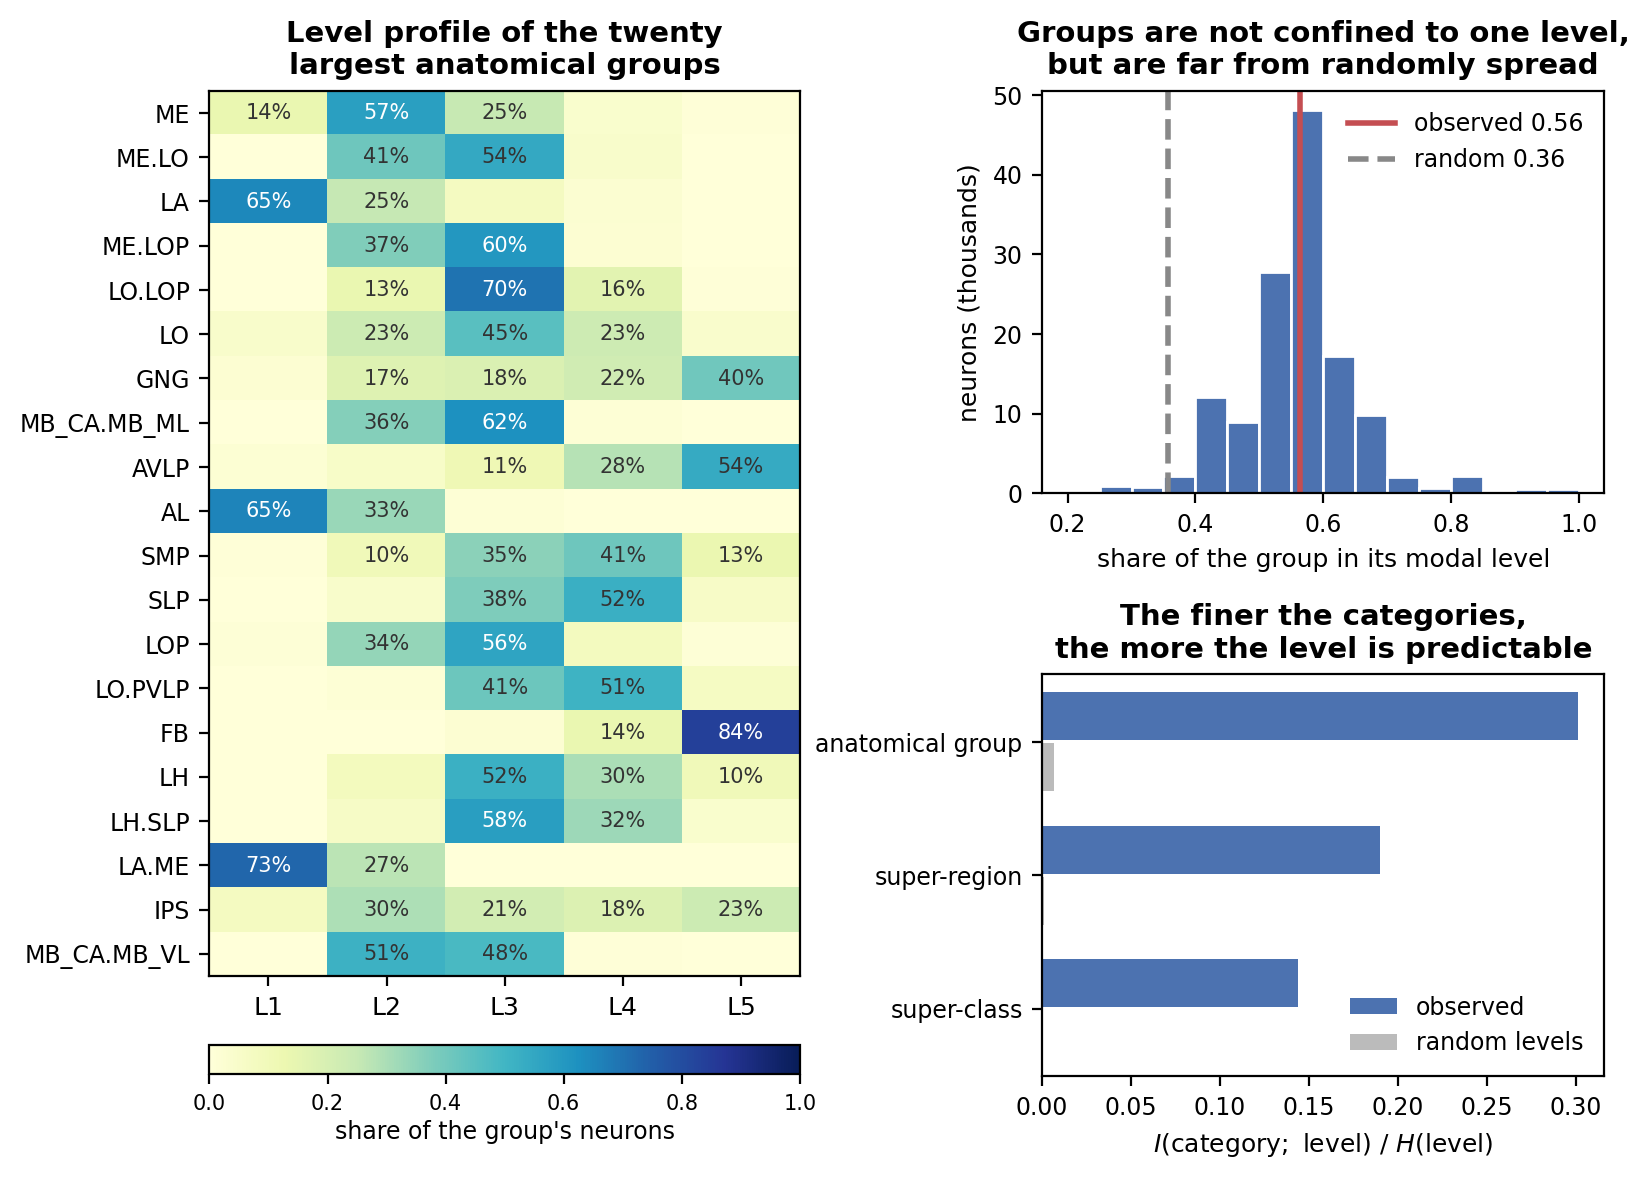
\includegraphics[width=0.88\textwidth]{level_coherence.png}
\caption[Coherence between anatomical group and level]{How anatomical
categories distribute over the hierarchical levels. On the left, the level
profile of the twenty largest anatomical groups, each row normalised to its
own population: the mass of a group concentrates on adjacent levels rather
than spreading uniformly, and the lobula plate is visible as a structure
straddling levels~2 and~3. In the centre, the distribution of purity over all
$628$ groups weighted by population, against the value obtained when levels
are assigned at random. On the right, the normalised mutual information
between category and level at the three granularities: the finer the
categorisation, the more the level is determined, which is the opposite of
what one would expect if the layering were an artefact of the super-class
labels it was calibrated on.}
\label{fig:level-coherence}
\end{figure}

One caveat should be recorded. All three quantities are computed on the
levels as given, and none of them validates the level construction itself;
they establish only that the construction is at least as compatible with the
anatomical group as with the categorisation used to build it.

Nor does the functional gradient of Section~\ref{sec:results-hierarchy}
supply the missing validation, for the reason given there: the level
boundaries were chosen to separate super-classes, so finding that the levels
separate super-classes is not an independent test. What that gradient does
support is the \emph{spectral embedding} underlying the levels, since four
thresholds on a fixed axis could not have produced it had the axis not
already carried the ordering. The discretisation itself remains a modelling
choice inherited from earlier work, and no result in this thesis tests it.

\subsection{The Macro-Scale Hourglass}
\label{sec:results-macro}

Table~\ref{tab:hscore} reports the hourglass score under both routing
schemes and several bounds on path length, all at $\tau = 0.9$.

\begin{table}[H]
\centering
\caption{Hourglass score under different routing schemes and path-length
bounds, at $\tau = 0.9$. The last row is degenerate and is reported to show
why the bound is mandatory.}
\label{tab:hscore}
\begin{tabular}{llrrrr}
\toprule
Routing & Max hops & $S \to T$ paths & $|C(\tau)|$ & $|C_f(\tau)|$ & $H$ \\
\midrule
\code{levels} & 4 (structural) & 1,995,460   & 154 & 307 & \textbf{0.498} \\
\code{score}  & 3              & 4,236,294   & 331 & 456 & 0.274 \\
\code{score}  & 4              & $1.20\times10^{8}$ & 326 & 433 & 0.247 \\
\code{score}  & 5              & $3.67\times10^{9}$ & 269 & 401 & 0.329 \\
\code{score}  & $\infty$       & $1.17\times10^{75}$ & 1 & 10 & \emph{(degenerate)} \\
\bottomrule
\end{tabular}
\end{table}

Under structural routing the score is $0.498$, which is to say that the real
core is half the size that the dependency structure alone would require. By
the definition of Equation~\eqref{eq:hscore} the hourglass property is
therefore present, and Figures~\ref{fig:hscore-curve}
and~\ref{fig:coverage-curve} show that the finding does not hinge on the
particular threshold chosen.

\begin{figure}[H]
\centering

\includegraphics[width=0.78\textwidth]{hscore_curve.png}
\caption[Hourglass score across coverage thresholds]{Hourglass score as a
function of the coverage threshold $\tau$, under level-based routing. The
score is stable over a broad range of $\tau$, which is what makes the single
value reported at $\tau = 0.9$ meaningful rather than an artefact of one
threshold.}
\label{fig:hscore-curve}
\end{figure}

\begin{figure}[H]
\centering

\includegraphics[width=0.78\textwidth]{coverage_curve.png}
\caption[Cumulative path coverage]{Cumulative fraction of sensory-to-motor
paths covered as neurons are added to the core in decreasing order of path
centrality. The sharp initial rise is the hourglass property in its rawest
form: $154$ neurons out of $134{,}181$ carry $90\%$ of the end-to-end
flow.}
\label{fig:coverage-curve}
\end{figure}

The score is nevertheless routing-dependent, ranging from $0.247$ to
$0.498$ across the schemes tested, and the honest way to report it is
therefore the full table rather than any single figure drawn from it. The
final row of the table shows what happens when the bound on path length is
removed altogether: the count of source-to-target paths reaches
$1.17 \times 10^{75}$, a single neuron then covers $97.6\%$ of them, and the
$\tau$-core collapses to one element. At that point the measure has lost all
content, which is the concrete justification for the requirement stated in
Section~\ref{sec:macro-methods}.

That the observed concentration is not an artefact of the degree sequence
was checked directly against randomised networks, as
Figure~\ref{fig:null-hscore} shows.

\begin{figure}[H]
\centering

\includegraphics[width=0.72\textwidth]{null_hscore.png}
\caption[Null distribution of the hourglass score]{Distribution of the
hourglass score over randomised networks, against the observed value. The
observed score falls well outside the null distribution, establishing that
the concentration of flow is not a by-product of the degree sequence
alone.}
\label{fig:null-hscore}
\end{figure}

\subsubsection{Weaker Than in \textit{C.\ elegans}, and Why That May Be
Expected}

The reference study of Sabrin et al.\ \cite{sabrin2020} reports hourglass
scores between $0.74$ and $0.87$ for the \textit{C.\ elegans} connectome.
The values obtained here, between $0.25$ and $0.50$, are substantially
lower. The \Dros{} brain is therefore hierarchically organised, but it
funnels its flow through a narrow waist considerably less than the nematode
does, and the difference is large enough to require an explanation rather
than a remark.

A plausible one, offered here as an argument to be weighed rather than as a
demonstrated result, is that the two nervous systems are solving different
problems. \textit{C.\ elegans} routes essentially all of its sensory
information through ten to fifteen command interneurons, an interneuron being
a neuron that sits between others rather than receiving from a sense organ or
driving a muscle; those few cells constitute a single shared bottleneck for
the whole animal. The fly processes several
sensory modalities in parallel, and each of them plausibly has its own
bottleneck rather than sharing one. The composition of the $\tau$-core
supports this reading, since it separates into distinct clusters, with
\code{AL} structures serving olfaction, \code{GNG} and \code{PRW} serving
taste and mechanosensation, and \code{LH.SLP} forming a third group, rather
than forming a single shared core. Several parallel hourglasses will
necessarily produce a lower global score than one deep hourglass, even when
each individual pathway is strongly funnelled, because the union of several
small cores is larger than any one of them.

\subsection{Bow-Tie Motifs Across Level Windows}
\label{sec:results-windows}


This section reports the exhaustive motif search. It covers the four level
windows and what changes between them, the decomposition of the patterns by
directional signature, and the distribution of the mass across chains of
levels, which is what locates the waist within the hierarchy.

The organising finding is that the architecture is not uniform with depth.
The shallow and the deep brain differ not in how many patterns they contain
but in what kind, and the difference is large enough that reporting a single
window would have given a misleading picture of the connectome.

\subsubsection{The Four Windows}

Table~\ref{tab:windows} summarises the exhaustive search over all four level
windows, which to our knowledge has not previously been carried out on this
connectome.

\begin{table}[H]
\centering
\caption{Exhaustive bow-tie motif search across level windows, with
$\kin=\kout=2$, $\mathit{max\_jump}=1$ and $\mathit{min\_count}=10$.}
\label{tab:windows}
\begin{tabular}{lrrrr}
\toprule
Window & Neurons & Metanodes & Motifs & Runtime \\
\midrule
$\{1,2,3\}$     & 104,915 &  879 & 31,184,800  & 14m39s \\
$\{2,3,4\}$     & 108,438 & 1155 & 119,026,375 & 57m43s \\
$\{3,4,5\}$     &  73,531 & 1220 & 433,546,629 & 3h05m51s \\
$\{1,2,3,4,5\}$ & 134,181 &  --- & 512,969,374 & 3h34m49s \\
\bottomrule
\end{tabular}
\end{table}

The motif count grows steeply with depth, from thirty-one million through
one hundred and nineteen million to four hundred and thirty-four million,
while the number of neurons does not grow at all: the deepest window
contains fewer neurons than the shallowest.
Figure~\ref{fig:window-growth} makes the dissociation visible. Growth is
therefore driven by connection density rather than by the size of the search
space, exactly as the density measurements of
Section~\ref{sec:results-hierarchy} would predict.

\begin{figure}[H]
\centering
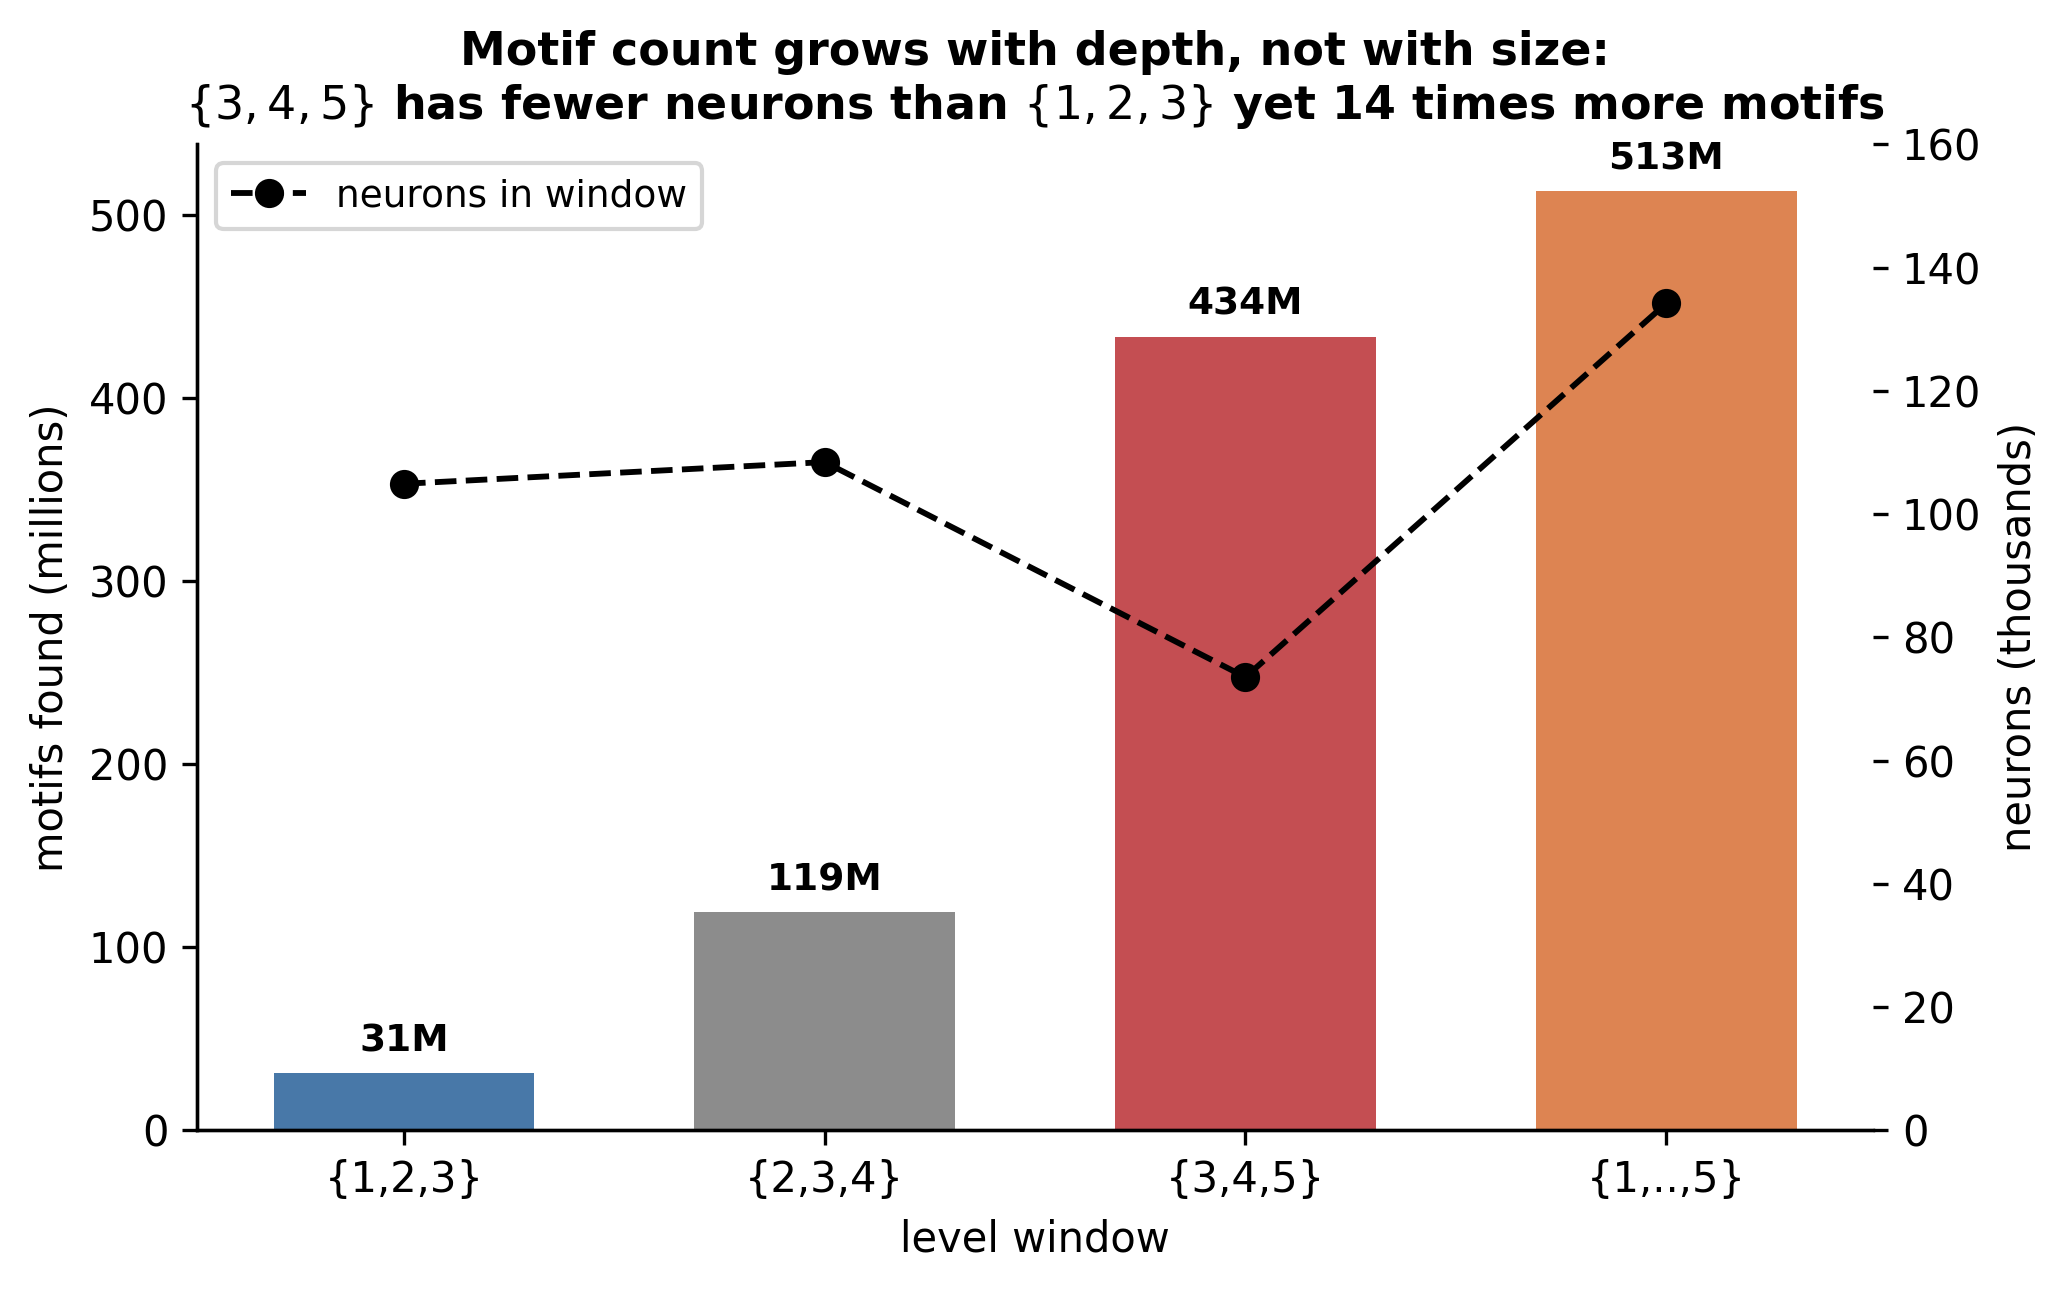
\includegraphics[width=0.86\textwidth]{window_growth.png}
\caption[Motif count and window size]{Number of bow-tie motifs found in each
level window, shown as bars against the left axis, together with the number
of neurons the window contains, shown as a dashed line against the right
axis. The two do not track each other: window $\{3,4,5\}$ contains fewer
neurons than $\{1,2,3\}$ yet yields fourteen times as many motifs.}
\label{fig:window-growth}
\end{figure}

The scale of the pruning described in Section~\ref{sec:micro-methods} can be
read off the shallow window, where the search examined $8{,}310{,}710{,}163$
candidate combinations. Of these, $112{,}688{,}248$ were excluded by the
disjointness constraint and $8{,}125{,}079{,}064$ were discarded because one
of their flow factors was identically zero, leaving $72{,}942{,}851$ raw
motifs of which $31{,}184{,}800$ passed the minimum count threshold. More
than ninety-seven per cent of the nominal space is thus eliminated without
any loss of exactness.

\subsubsection{Directional Signatures}
\label{sec:results-signature}

Section~\ref{sec:motifs} set out why the motifs are classified by the
signature of Equation~\eqref{eq:signature} rather than by the agreement of
all four edges at once. What that section could not show is how the thirteen
classes hidden inside the coarse \emph{mixed} label actually behave, and they
turn out to differ considerably, as Figure~\ref{fig:signature-distrib}
shows.

\begin{figure}[H]
\centering

\includegraphics[width=\textwidth]{signature_distrib.png}
\caption[Directional signature distribution]{Decomposition of the sixteen
directional signatures on window $\{1,2,3\}$, by number of patterns on the
left and by share of total count mass on the right. The two panels disagree
substantially: \code{mix->FWD} is frequent but carries almost no mass, while
\code{FWD->mix} is the reverse. The pure signatures \code{FWD->FWD} and
\code{BWD->BWD} are highlighted, and their rarity is what makes the coarse
four-way classification uninformative.}
\label{fig:signature-distrib}
\end{figure}

The two panels of that figure disagree in an instructive way. A signature
may account for many distinct patterns while contributing almost nothing to
the total count, as \code{mix->FWD} does, or account for relatively few
patterns each of which is realised enormously often, as \code{FWD->mix} does.
Reporting only one of the two quantities would therefore give a misleading
picture, and both are reported throughout.

Comparing the shallow and deep windows reveals that this composition is not
a fixed property of the connectome but changes substantially with depth.

\begin{table}[H]
\centering
\caption{Share of total motif mass by directional signature, shallow versus
deep window. The upper block lists every signature in which at least one
branch is entirely lateral, that is, in which \emph{both} edges entering the
waist, or \emph{both} edges leaving it, run within a single level; the lower
block gives the two largest signatures without such a branch. The seven
signatures omitted from the table carry $10.2\%$ of the shallow mass and
$2.1\%$ of the deep mass between them.}
\label{tab:signatures}
\begin{tabular}{lrr}
\toprule
Signature & $\{1,2,3\}$ (\% mass) & $\{3,4,5\}$ (\% mass) \\
\midrule
\code{LAT->mix}  &  9.2 & \textbf{42.7} \\
\code{mix->LAT}  & 10.3 & \textbf{23.3} \\
\code{FWD->LAT} & 11.9 &  0.4 \\
\code{LAT->LAT}  &  0.6 & \textbf{10.2} \\
\code{LAT->BWD} &  6.0 &  0.2 \\
\code{LAT->FWD} &  0.0 &  3.7 \\
\code{BWD->LAT} &  0.0 &  2.1 \\
\midrule
\emph{all seven of the above} & \emph{38.0} & \textbf{\emph{82.6}} \\
\midrule
\code{mix->mix}  & \textbf{38.5} & 13.9 \\
\code{FWD->mix}  & 13.3 &  1.5 \\
\bottomrule
\end{tabular}
\end{table}

Signatures containing at least one purely lateral branch carry $38.0\%$ of
the mass in the shallow window and $82.6\%$ in the deep one, while
\code{mix->mix}, which dominates the shallow window at $38.5\%$, falls to
$13.9\%$. What changes with depth is not only how much of the mass is
lateral but which kind: in the shallow window the lateral branch is usually
paired with a forward or backward one, as in \code{FWD->LAT} at $11.9\%$,
whereas in the deep window it is almost always paired with a mixed branch or
with another lateral one. Figure~\ref{fig:signature-shift} displays the same comparison
signature by signature, sorted by the magnitude of the shift. The deep brain
is, in this precise sense, laterally dominated: its characteristic circuit
is one in which information enters or leaves a waist by moving sideways
within a processing stage rather than by advancing through the hierarchy.

\begin{figure}[H]
\centering
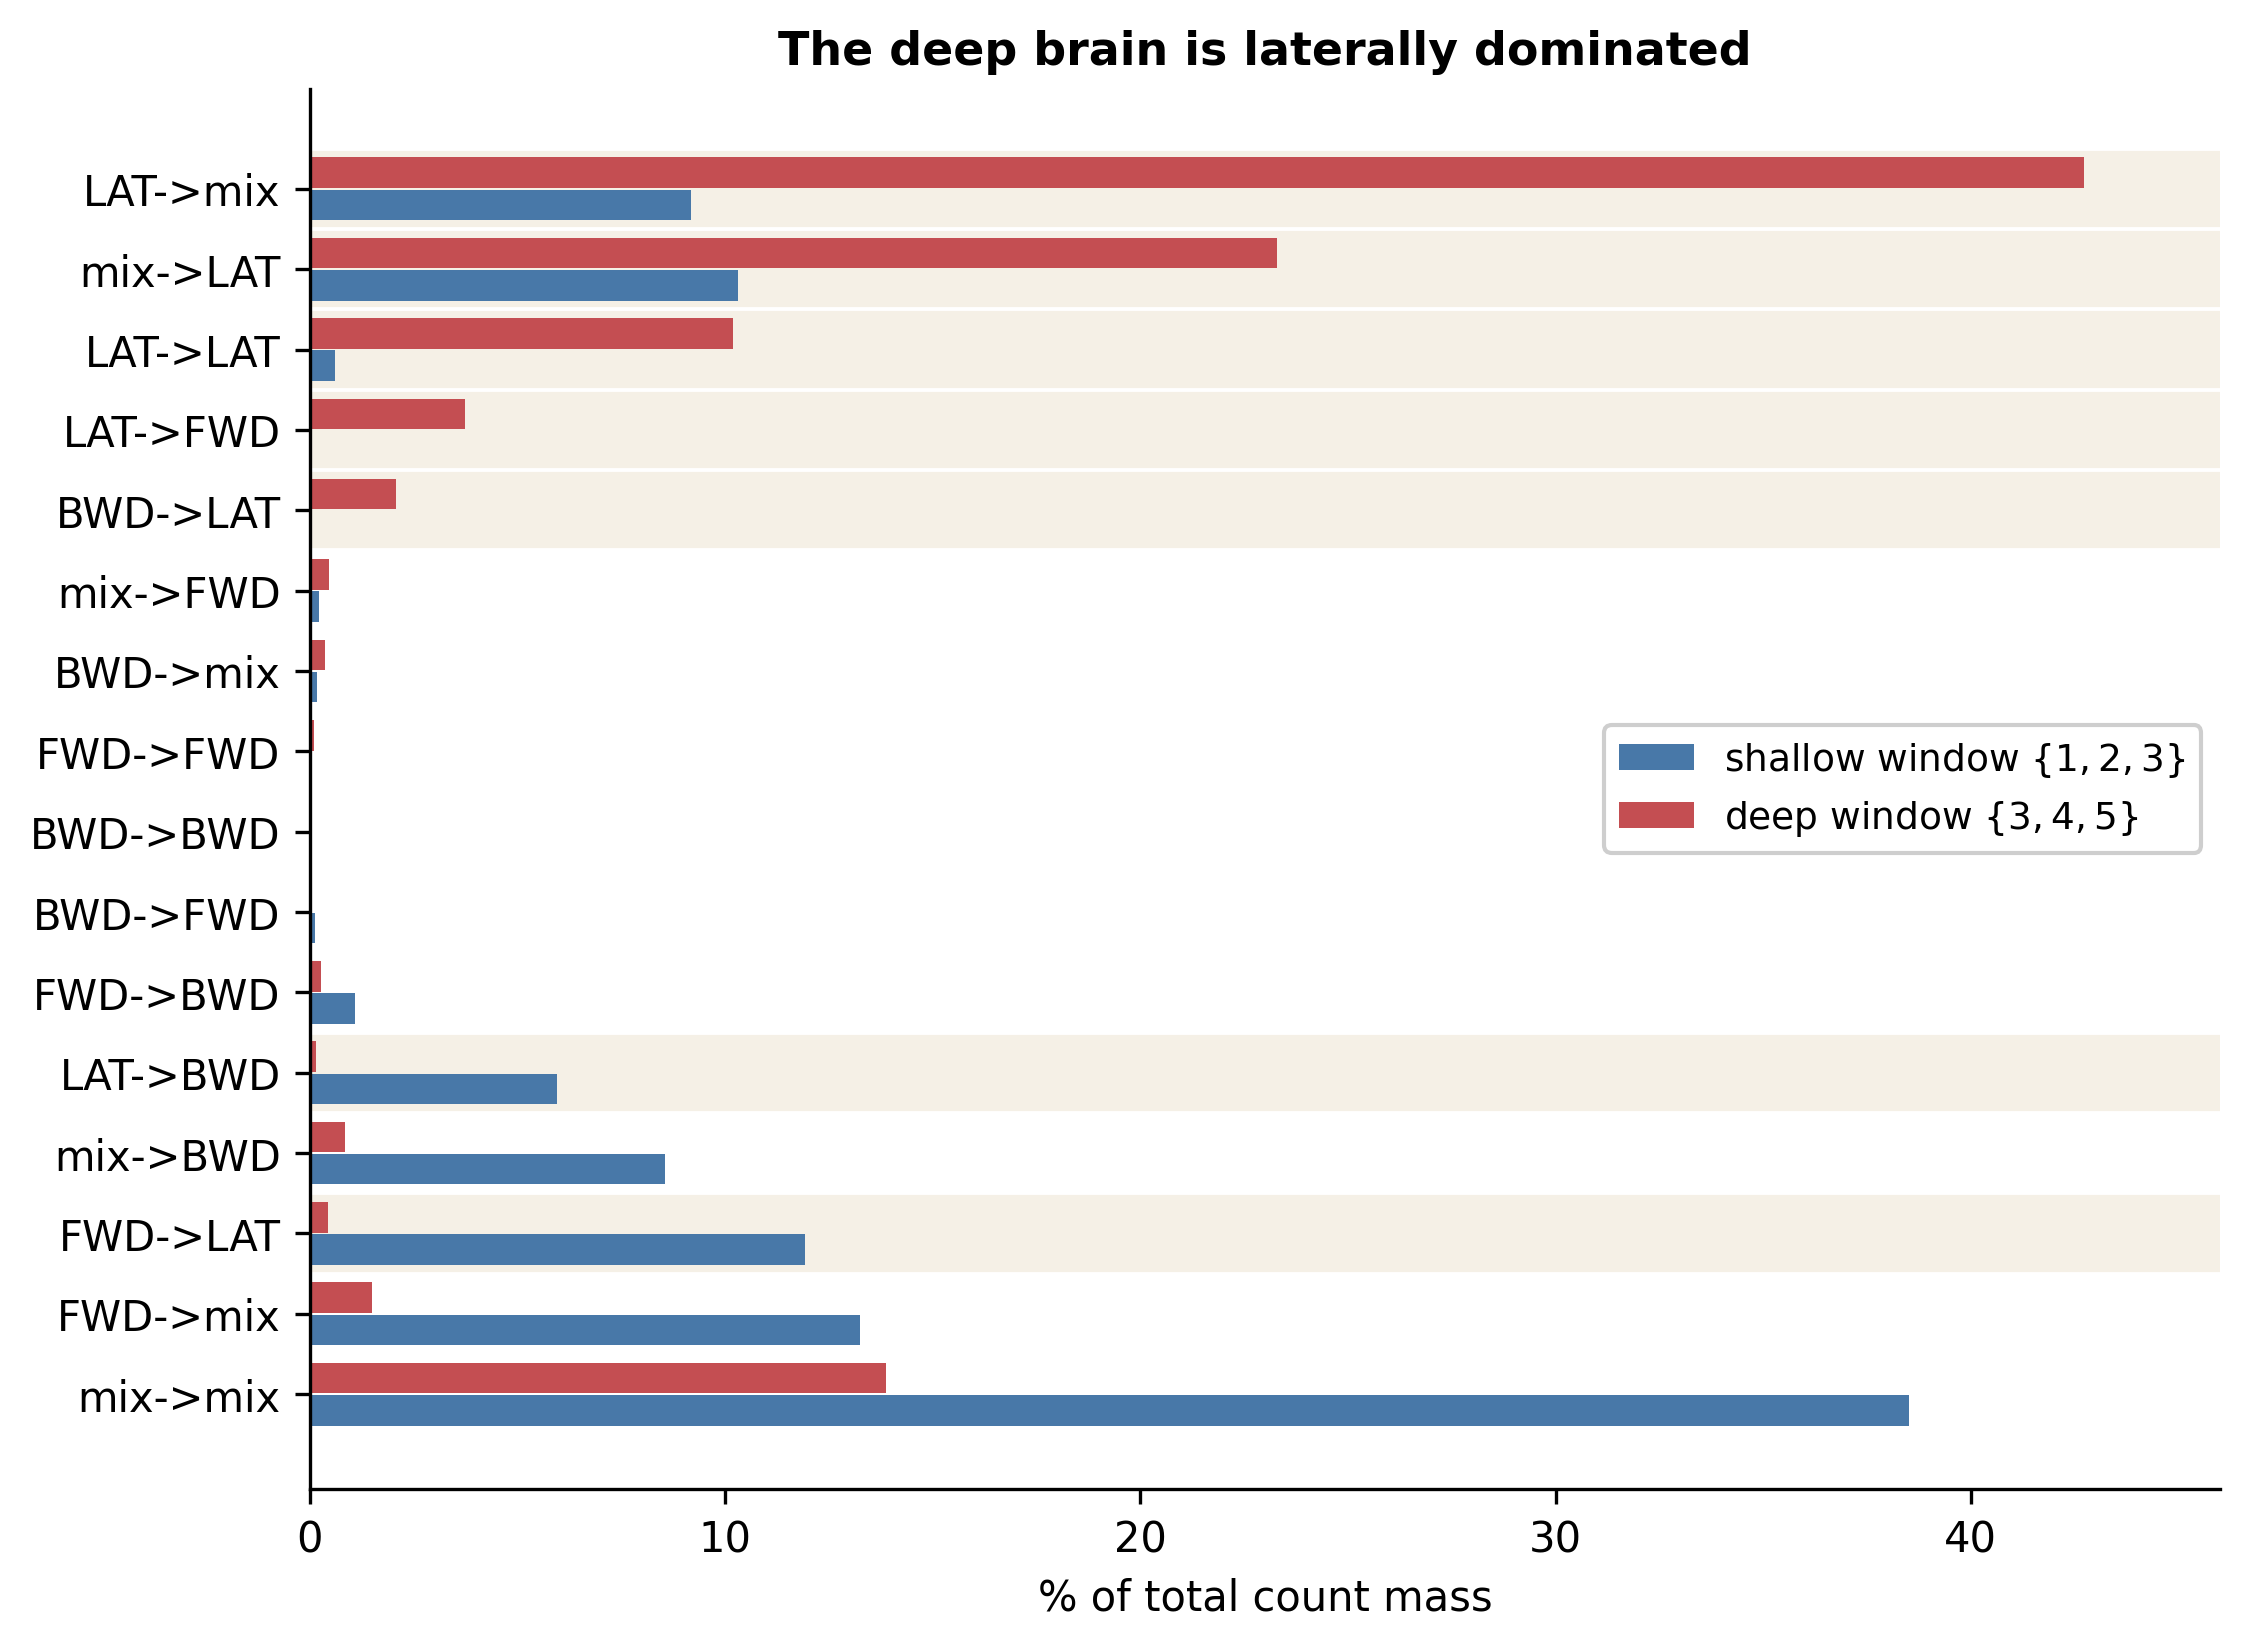
\includegraphics[width=0.92\textwidth]{signature_shift.png}
\caption[Signature composition, shallow versus deep]{Share of total count
mass by directional signature in the shallow and deep windows, sorted by the
size of the shift between them. Shaded rows are signatures containing a
purely lateral branch, and they gain almost exactly what the others lose.
\code{LAT->mix} alone rises from $9.2\%$ to $42.7\%$.}
\label{fig:signature-shift}
\end{figure}

The highest-count individual patterns illustrate the same point concretely.
Figure~\ref{fig:motif-top1} shows the single most frequent bow-tie of the
shallow window, and Figures~\ref{fig:motif-catalog-1}
to~\ref{fig:motif-catalog-4} give representative examples of every signature
class.

\begin{figure}[H]
\centering
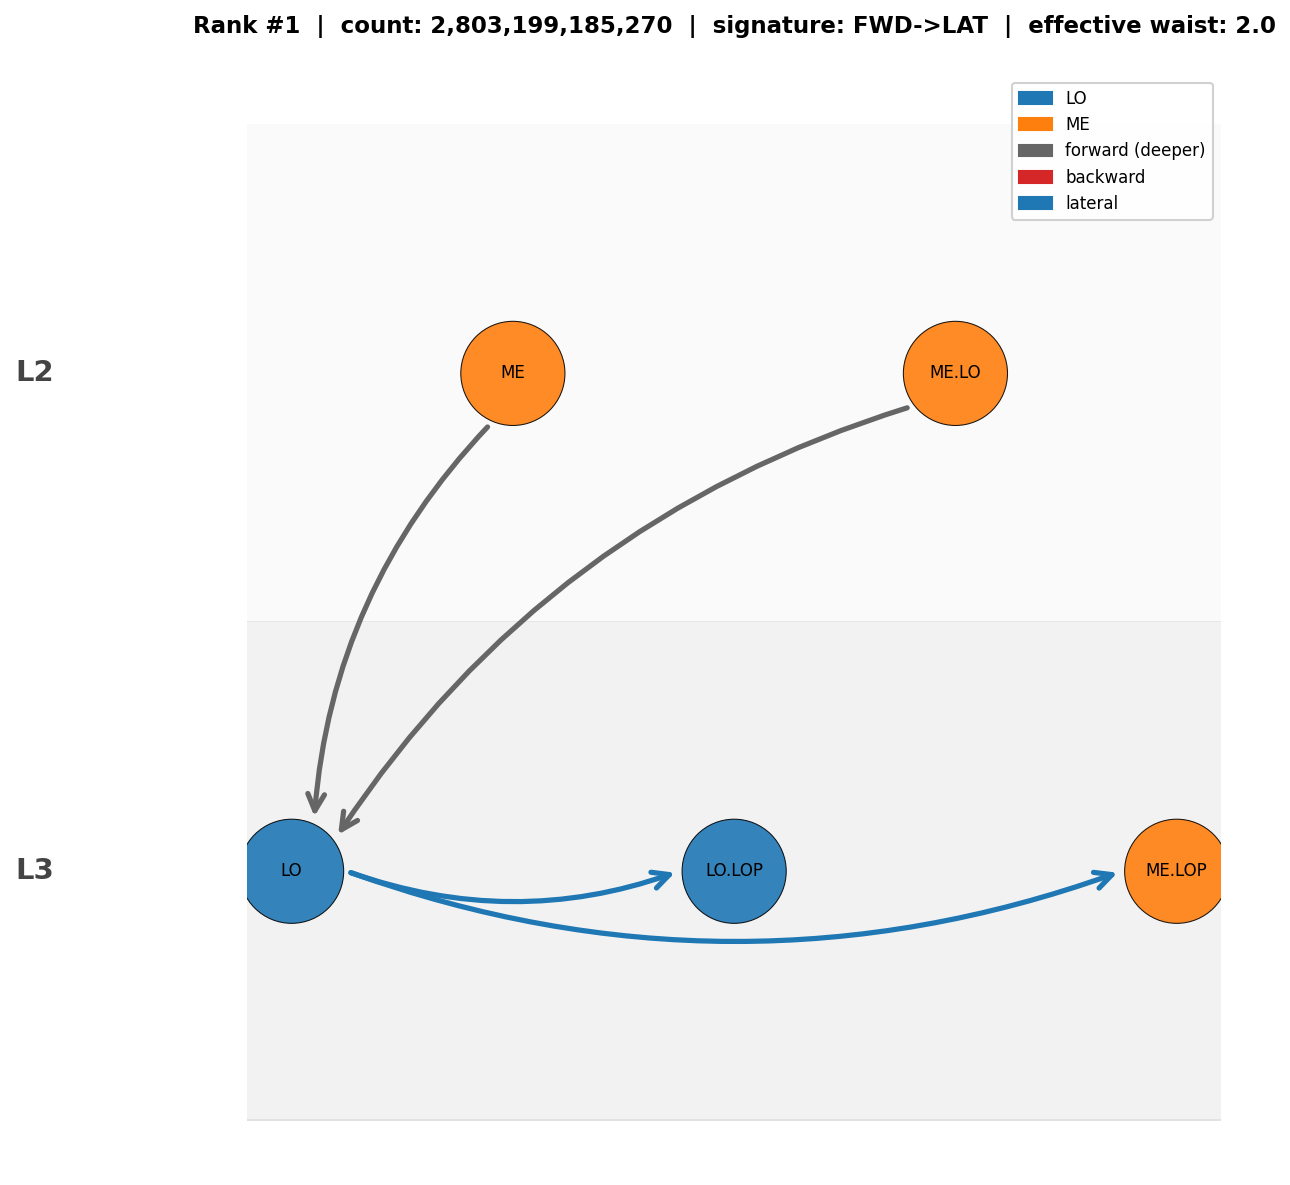
\includegraphics[width=0.92\textwidth]{motif_top1.png}
\caption[The most frequent bow-tie motif]{The single most frequent bow-tie
motif of window $\{1,2,3\}$, with $2.80 \times 10^{12}$ instances and
signature \code{FWD->LAT}. The vertical axis is the hierarchical level, with
depth increasing downwards and each level drawn as a shaded band, so that the
direction of an edge is given by its slope: an edge that descends runs
forward, one that rises runs backward, and a horizontal one is lateral. Two
medulla groups at level~2 converge onto the lobula at level~3, which then
distributes laterally within level~3. Grey edges are forward and blue edges
lateral. The pattern is a compact illustration of the general finding: the
dominant structures combine a forward entry with a lateral spread rather than
being purely forward.}
\label{fig:motif-top1}
\end{figure}

\begin{figure}[H]
\centering

\includegraphics[width=0.86\textwidth]{hourglass_catalog_1.png}
\caption[Representative motifs by signature, part 1]{Representative bow-tie
motifs for the first four directional signatures, window $\{1,2,3\}$. The
horizontal axis carries the role a group plays in the motif, with the input
groups on the left, the waist in the centre and the output groups on the
right; the vertical axis carries the hierarchical level, drawn as shaded
bands labelled at the left margin, with depth increasing downwards. The two
axes together make the structure legible from the shape alone: an edge that
descends is forward, one that rises is backward, and a horizontal one is
lateral, so the signature can be read without consulting the node labels.
Labels give the anatomical group, node colour encodes the macro-area, and
edge colour repeats the direction, with grey for forward, red for backward
and blue for lateral. The counts above each panel are numbers of neuron-level
instances, and they differ between classes by nearly three orders of
magnitude.}
\label{fig:motif-catalog-1}
\end{figure}

\begin{figure}[H]
\centering

\includegraphics[width=0.86\textwidth]{hourglass_catalog_2.png}
\caption[Representative motifs by signature, part 2]{Representative motifs,
signatures five to eight, with conventions as in
Figure~\ref{fig:motif-catalog-1}. The optic-lobe groups dominate the
highest-count patterns throughout, consistent with the density reported in
Section~\ref{sec:results-hierarchy}.}
\label{fig:motif-catalog-2}
\end{figure}

\begin{figure}[H]
\centering

\includegraphics[width=0.86\textwidth]{hourglass_catalog_3.png}
\caption[Representative motifs by signature, part 3]{Representative motifs,
signatures nine to twelve, with conventions as in
Figure~\ref{fig:motif-catalog-1}.}
\label{fig:motif-catalog-3}
\end{figure}

\begin{figure}[H]
\centering

\includegraphics[width=0.86\textwidth]{hourglass_catalog_4.png}
\caption[Representative motifs by signature, part 4]{Representative motifs,
the remaining signatures, with conventions as in
Figure~\ref{fig:motif-catalog-1}.}
\label{fig:motif-catalog-4}
\end{figure}

\subsubsection{Level Chains}

A complementary view attributes the mass of each pattern to the triple
consisting of the level of its inputs, the level of its waist and the level
of its outputs. This is coarser than the signature, since it records only
which levels are involved rather than how the branches are oriented, but it
answers a question the signature cannot: where in the hierarchy the
bottlenecks actually sit.

In the deep window the dominant chains are L3 to L3 to L3 at $45.6\%$ of the
mass, L3 to L3 to L4 at $28.0\%$, L4 to L3 to L3 at $16.6\%$ and L4 to L3 to
L4 at $3.3\%$, as Figure~\ref{fig:level-chains} shows.

\begin{figure}[H]
\centering
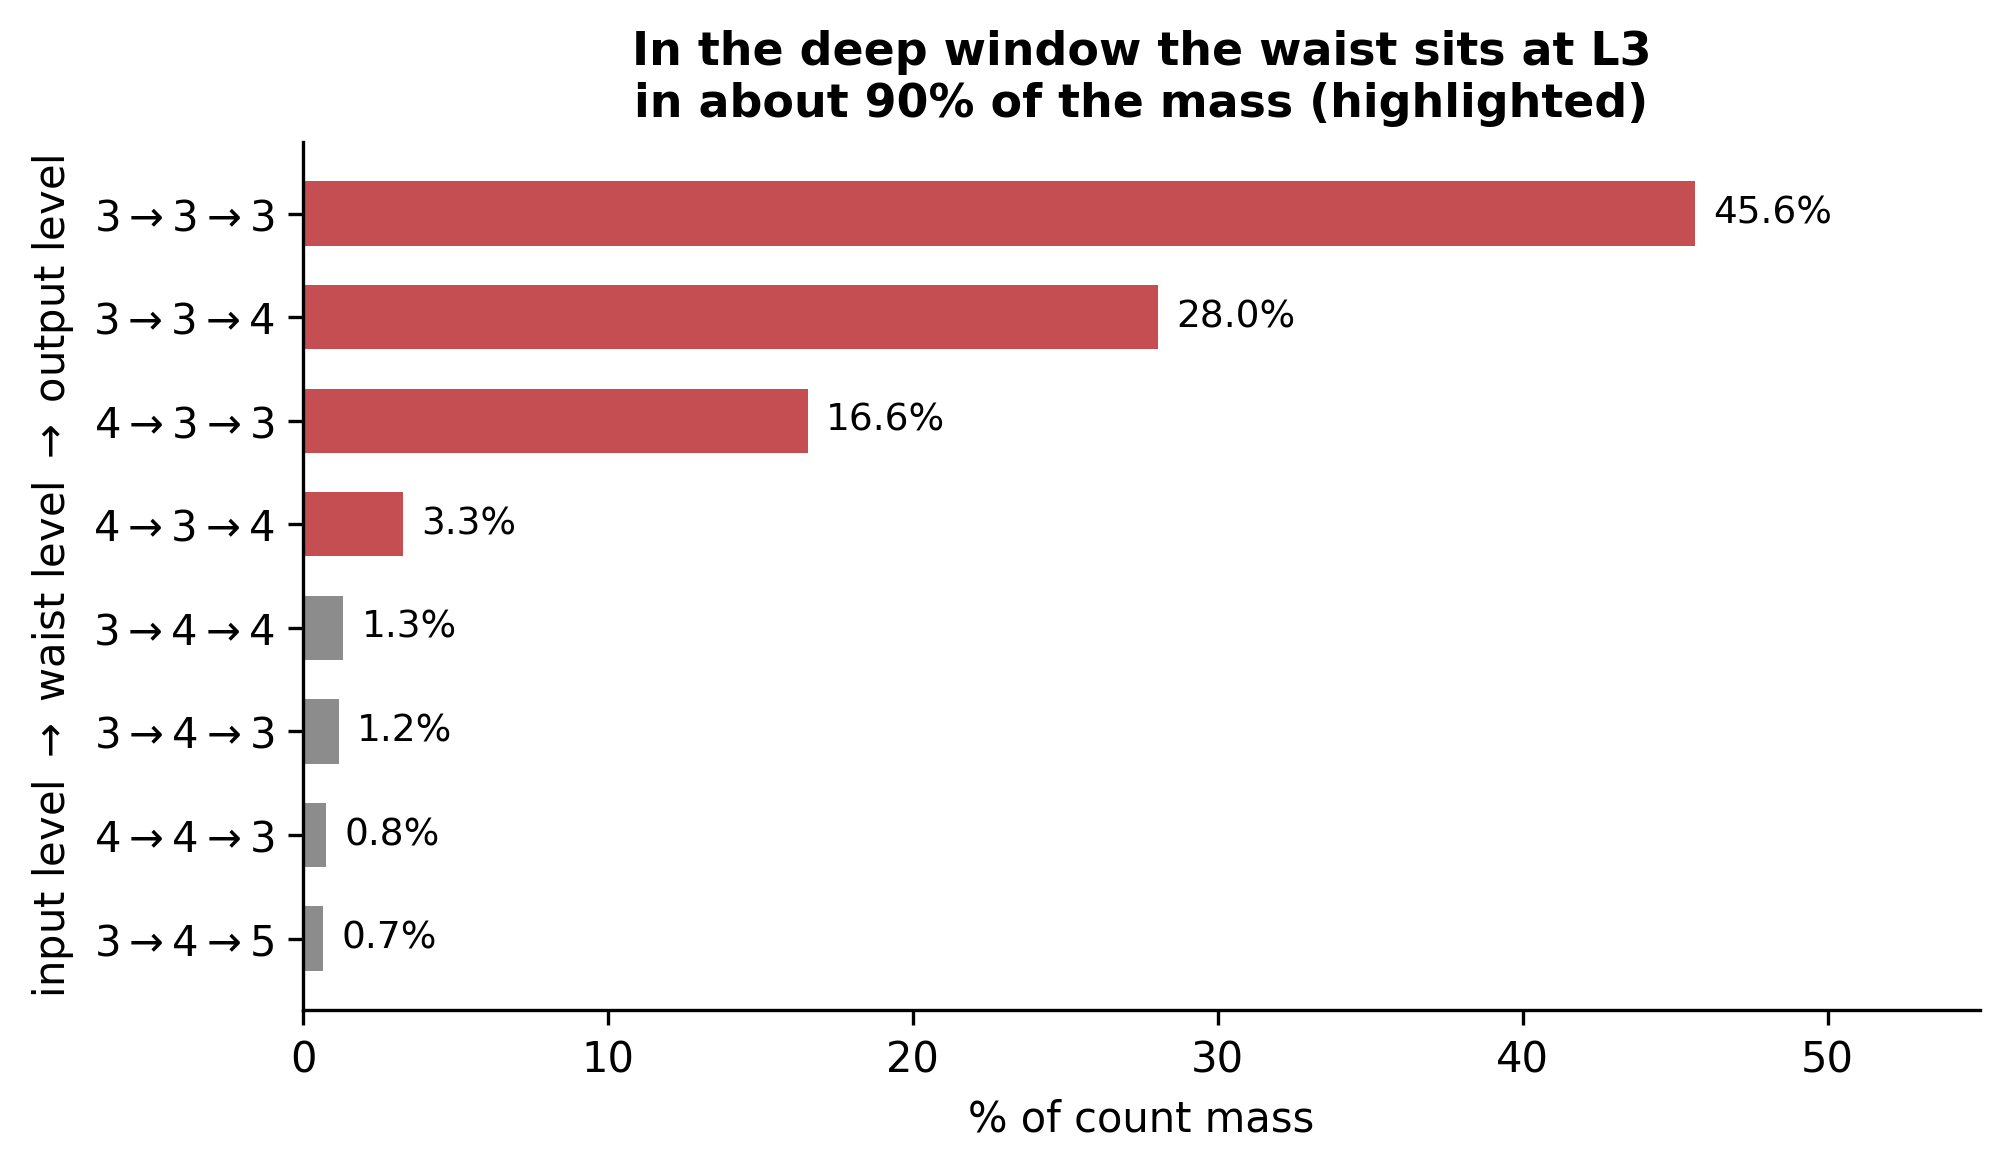
\includegraphics[width=0.80\textwidth]{level_chains.png}
\caption[Mass distribution across level chains]{Distribution of motif mass
across level chains in the deep window, where a chain records the input
level, the waist level and the output level. Chains whose waist lies at
level~3 are highlighted, and together they account for roughly $90\%$ of the
mass.}
\label{fig:level-chains}
\end{figure}

The waist sits at level~3 in roughly ninety per cent of the mass. That the
bottleneck is in the middle of the hierarchy is the expected outcome rather
than a surprising one, and it is worth saying why before drawing anything
further from the table.

A bow-tie requires convergence on its way in and divergence on its way out.
Neither is available at the ends of the hierarchy. Level~1 is dominated by
sensory neurons, which receive almost nothing from inside the brain and so
cannot be converged upon; level~5 is dominated by descending and motor
neurons, which project out of the brain and so have little to diverge into
within it. The middle is the only place where a neuron has both a substantial
input from within the network and a substantial output back into it, and it
is also, for the same reason, where the processing happens. Finding the waist
there therefore does not so much reveal something unexpected about the
connectome as confirm that the measure is picking up processing structure
rather than an artefact of how the levels were drawn. It is the result one
would want to see before trusting anything else the search reports.

What is not automatic is which of the middle levels it turns out to be, and
how sharply. Level~5 is the most internally dense level of the entire
connectome, as Section~\ref{sec:results-hierarchy} established, and yet it
barely appears as a waist at all. High internal density combined with very
few bottlenecks is a specific structural signature: it indicates connectivity
that is recurrent and lateral rather than convergent and divergent. A region
can be densely wired without any of its neurons functioning as an obligatory
passage point, and level~5 appears to be exactly such a region. That
distinction is invisible to density measurements taken on their own, and it
is one of the clearer instances in this work of the two scales of analysis
saying different things about the same tissue.

\subsubsection{The Shallow Window, and a Direct Answer About L1}

The same analysis on the shallow window gives a sharper picture still, in
which four chains account for $99.2\%$ of the entire count mass.

\begin{table}[H]
\centering
\caption{Level chains in the shallow window: four chains carry almost all
the mass, and all four have their waist at level~3.}
\label{tab:chains-shallow}
\begin{tabular}{lr}
\toprule
Chain & Share of mass \\
\midrule
L2 $\to$ L3 $\to$ L3 & 33.3\% \\
L3 $\to$ L3 $\to$ L2 & 24.4\% \\
L2 $\to$ L3 $\to$ L2 & 21.6\% \\
L3 $\to$ L3 $\to$ L3 & 19.9\% \\
\midrule
\textbf{total} & \textbf{99.2\%} \\
\bottomrule
\end{tabular}
\end{table}

All four have their waist at level~3, the same concentration observed
independently in the deep window and therefore not a peculiarity of either.
Two windows sharing only one level agree on where the bottleneck sits, which
is a stronger statement than either window makes alone.

The table also answers directly a question that motivated this part of the
analysis, namely how many bow-tie patterns run from level~1 into level~2.
The answer is that almost none do. Every chain involving level~1 together
accounts for roughly $0.02\%$ of the mass, despite level~1 containing
$13{,}601$ neurons. The explanation is functional rather than an artefact of
the method: level~1 is $94\%$ photoreceptors and sensory neurons, which
receive very little from within the brain and project forward. They are
sources of flow rather than points of convergence, and a bow-tie requires
convergence. A neuron population can therefore be large and still be a poor
waist, which is a useful corrective to the intuition that the biggest
structures must be the most important ones.

\subsection{What the Choice of Granularity Recovers}
\label{sec:results-granularity}

Section~\ref{sec:groups} argued for grouping neurons by anatomical group
rather than by functional super-class or by super-region. Since that choice
conditions every result in this chapter, and since the coarsest of the three
is the one adopted in the previous work of Section~\ref{sec:related}, the
entire search was repeated at both of the other granularities on the shallow
window, so that the comparison could be made on results rather than in the
abstract. The three runs differ only in the map from neurons to categories;
the window, the parameters, the engine and the pruning are identical.

\begin{table}[H]
\centering
\caption{The same search on window $\{1,2,3\}$ under the three
categorisations. Categories counts the values present in the window, and
metagraph edges counts distinct ordered pairs of metanodes joined by at least
one synapse within one level of each other.}
\label{tab:granularity}
\begin{tabular}{lrrr}
\toprule
 & super-class & super-region & anatomical group \\
\midrule
categories in window      & 9      & 76        & 477 \\
metanodes                 & 24     & 188       & 879 \\
metagraph edges           & 293    & 6{,}295   & 24{,}914 \\
median neurons / metanode & 511    & 11        & 3 \\
distinct waists           & 20     & 157       & 660 \\
motifs found              & 29{,}091 & 4{,}923{,}197 & 31{,}184{,}800 \\
runtime                   & 6.7\,s & 2m31s     & 14m39s \\
\bottomrule
\end{tabular}
\end{table}

The first thing to report is what the coarse analysis does \emph{not} do,
because it contradicts an argument that might be expected. One could suppose
that super-class granularity is unusable because its metanodes are too large
to be waists: the largest, \emph{optic} at level~2, contains $35{,}584$
neurons, a quarter of the network. That supposition is wrong. The waist
carrying the most mass in the coarse run is \emph{visual centrifugal} at
level~2, a metanode of only $311$ neurons with an effective size of $3.9$.
Narrow waists emerge perfectly well at coarse granularity, because what
produces a high count is convergence and divergence structure, not
population. The coarse analysis is also very cheap, finishing in under seven
seconds and yielding twenty-nine thousand patterns rather than thirty-one
million, which makes it far easier to inspect by hand.

What the coarse analysis loses is anatomical resolution, and the clearest way
to see it is to put the leading pattern of the three runs side by side. At
super-class granularity the most frequent bow-tie reads
\[
[\text{central L1},\ \text{central L2}] \rightarrow
\text{visual centrifugal L2} \rightarrow
[\text{optic L1},\ \text{optic L2}],
\]
which says that central neurons converge on visual centrifugal neurons that
project to optic ones. At super-region granularity it reads
\[
[\code{AL\_L1},\ \code{AL\_L2}] \rightarrow \code{AL.MB\_L2} \rightarrow
[\code{MB\_L2},\ \code{MB\_L3}],
\]
which is already a recognisable circuit: two antennal lobe populations
converge on neurons spanning the antennal lobe and the mushroom body, which
then project into the mushroom body. That is the olfactory pathway, and it is
the pathway on which several of the results of this chapter turn. At group
granularity the leading pattern reads
\[
[\code{ME\_L2},\ \code{ME.LO\_L2}] \rightarrow \code{LO\_L3} \rightarrow
[\code{LO.LOP\_L3},\ \code{ME.LOP\_L3}],
\]
which names a specific circuit within the optic lobe: two medulla populations
converge on the lobula, which distributes within its own level to the lobula
plate. All three statements are true of the same connectome; they differ in
how much they commit to.

The gap between the first and the other two is not a matter of degree. The
category \emph{central} contains $521$ distinct anatomical groups, and the
antennal lobe projection neurons, the Kenyon cells, the mushroom body output
neurons and the lateral horn all fall within it without exception. The
olfactory sequence just described therefore has every one of its stages
inside a single super-class node, and this is why the coarse run does not
merely rank it lower but cannot express it at all. The same holds for the
sequence reported in Section~\ref{sec:results-sweep}, in which projection
neurons broadcast onto Kenyon cells that then feed integrative output
neurons; for the compression results of Section~\ref{sec:results-compression},
which identify particular neuropils as bottlenecks; and for the recurrence
result of Section~\ref{sec:optic-recurrence}, which separates re-entry into
the lobula from relay through the lobula plate. None of these survives the
collapse of the central brain into one node.

The super-region granularity is the interesting middle case, because it
recovers most of what matters at a fraction of the cost. It is fine enough to
name the olfactory pathway, to separate the optic lobe from the central
complex and to distinguish the mushroom body from the lateral horn, and it
does so with $188$ metanodes rather than $879$ and in a sixth of the runtime.
What it cannot do is separate structures within a super-region: the calyx,
the pedunculus and the two lobes of the mushroom body are one node, so a
claim about where in the mushroom body a bottleneck sits is unavailable, and
the medulla, lobula and lobula plate are likewise merged, which is fatal to
the recurrence analysis of Section~\ref{sec:optic-recurrence}. It is the
right granularity for an overview and the wrong one for the questions this
thesis asks, but it is a genuinely useful third point of reference, and its
existence means the choice made here is not a binary one between an
unusable coarse view and an over-specific fine one.

\subsubsection{What the Abstraction Actually Buys}
\label{sec:abstraction-cost}

A fair objection to the fine granularity is that it weakens the abstraction
as a device for reducing complexity. If there are six hundred possible
categories per level, the metagraph starts to look less like a summary of the
connectome and more like a relabelling of it, and the reduction that
justified moving from neurons to metanodes in Section~\ref{sec:groups} is
correspondingly smaller. The objection is sound in direction, and the honest
answer is to quantify it rather than to deflect it.

On the shallow window the connectome contributes $104{,}915$ neurons and
$1{,}296{,}899$ distinct neuron-to-neuron connections within one level of
each other. The three abstractions reduce the nodes by factors of $4{,}371$,
$558$ and $119$ respectively, and the edges by factors of $4{,}426$, $206$
and $52$. The finest choice therefore still removes two orders of magnitude
from both, which is not nothing, but it removes a great deal less than the
coarsest one, and the number of metanodes it leaves, $879$, is of the same
order as the number of anatomical groups themselves. A reader who expected
the abstraction to leave a graph small enough to be inspected whole will not
find one.

Two things should be said in response. The first is that the reduction
matters less than it appears, because the search cost is not driven by the
number of metanodes but by the number of combinations of them around each
waist, and the pruning of Section~\ref{sec:pruning} removes most of those
before they are ever formed. The shallow window runs in fifteen minutes at
$879$ metanodes, so the abstraction is doing enough work to make an
exhaustive count feasible, which was its purpose.

The second, and the more important, is that reduction was never the only
objective. The abstraction has two jobs, and they pull against each other:
it must make the count tractable, and it must leave the result
interpretable. A metagraph of twenty-four nodes is maximally reduced and
tells us that \emph{central} neurons feed \emph{visual centrifugal} ones,
which is not a circuit. A metagraph of $879$ nodes is less reduced and tells
us that the medulla feeds the lobula, which is. The right measure of an
abstraction is not how much it compresses but how much of the compression it
achieves without destroying the distinctions the question depends on, and by
that measure the evidence in this section favours the finer choice, with the
super-region available as an intermediate whenever a coarser summary is
wanted. The three granularities are complementary rather than competing:
reporting all three costs less than three minutes of computation, and it
replaces an argument about which one is correct with a measurement of what
each one recovers.

\subsection{Waist Compression}
\label{sec:results-compression}

The nominal compression metric fails in exactly the way anticipated in
Section~\ref{sec:compression-methods}. Its ranking is headed by
\code{LO.PVLP\_L2}, which attains a nominal compression of $2431$ with only
\emph{two} active neurons out of twenty-one, while the biologically
prominent \code{AL.MB\_CA\_L2} scores merely $40$. The first of these is not
a bottleneck in any meaningful sense; it is a pair of neurons in a group
that happens to be large.

Under the realised metric of Equation~\eqref{eq:neff} the ranking becomes
interpretable. On the shallow window \code{AL.MB\_CA\_L2} has $144$ neurons
in its group, of which $118$ are active, an effective count of $4.8$, and
$2694$ peripheral neurons connected through it, giving a realised
compression of $561.8$. The metric now reflects the structure one wants it
to reflect, namely how much of the periphery is funnelled through how many
genuinely participating neurons.

On the deep window the analysis retains $19{,}416$ patterns, of which $794$
have an effective waist of at least five neurons, and the internal
consistency check described in Section~\ref{sec:verification} reproduced all
$19{,}416$ counts exactly. The leading structure there is \code{ME\_L4},
with a realised compression of $891.8$ over an effective waist of $5.7$
neurons, followed by several variants of \code{ME.LO\_L3}: the optic lobe
dominates compression in the deep brain as it dominates the motif counts.
Figure~\ref{fig:compression} plots the whole distribution.

\begin{figure}[H]
\centering

\includegraphics[width=0.82\textwidth]{compression.png}
\caption[Realised compression against effective waist size]{Realised
compression against the effective number of waist neurons for window
$\{3,4,5\}$, with the \code{ME.LO\_L3} family highlighted. Points at the far
left achieve high compression through a single active neuron and are
precisely the artefacts that the participation ratio is designed to expose.
A genuine bottleneck lies towards the upper right, having both many
effective neurons and high compression.}
\label{fig:compression}
\end{figure}

\subsubsection{Two Anatomically Distinct Forms of Recurrence}
\label{sec:optic-recurrence}

Restricting attention to the two recurrent signatures reveals something that
the aggregate figures conceal, namely that the two do not live in the same
place.

The re-entrant form, \code{FWD->BWD}, comprises $786{,}216$ patterns, which is
$2.52\%$ of the total, carrying a mass of $1.12 \times 10^{12}$ or $1.10\%$.
Its waist is the lobula, \code{LO\_L3}, in $88.5\%$ of that mass, and its
leading pattern has two medulla groups converging onto the lobula which then
projects onto two lobula plate groups. The relay form, \code{BWD->FWD},
comprises a very similar number of patterns, $822{,}466$, but carries nine
times less mass, and it sits on a different structure altogether: the lobula
plate, \code{LOP\_L2}, in $93.2\%$ of its mass. The purely backward form,
\code{BWD->BWD}, is negligible in mass and also lives on \code{LOP\_L2}.

The two forms of recurrence are therefore anatomically separated rather than
being two descriptions of one phenomenon. Re-entry into the lobula and relay
through the lobula plate are distinct circuits, and both belong to the optic
lobe, which dominates the recurrent structure of this window as it dominates
much else.

This dominance survives the correction of the compression metric, but it
must be qualified in one respect. Under realised compression the top of the
ranking remains optic, with \code{ME.LO\_L3} at $2173$, \code{ME.LO\_L2} at
$796$ and \code{ME\_L3} at $690$, but now with substantial counts, between
$4 \times 10^{5}$ and $1.4 \times 10^{7}$, and with genuine participation
rather than with two active neurons out of twenty-one. The dominance is thus
a property of the circuitry rather than an artefact of group size, which is
a stronger claim than the nominal metric could have supported.

\subsection{Statistical Significance}
\label{sec:results-validation}

Of the three hundred and twenty pre-registered patterns, all three hundred
and twenty had their observed counts reproduced exactly from the graph
before any testing began. After Benjamini--Hochberg correction at
$q < 0.05$, significance was obtained for $319$ of $320$ patterns under
model A and for $310$ of $320$ under both models B and C.

That the strictest model yields nearly the same number of significant
patterns as the weakest is the informative outcome. Model C preserves both
the block structure and the per-block degree sequences and randomises only
the alignment between them, so a pattern that remains significant under it
cannot be explained by degree sequences, nor by regional connection
densities, nor by which particular waist neurons happen to carry which
degrees. The convergence--divergence structure of these bow-ties is
therefore not accounted for by any of the three confounds tested.

\subsubsection{The Ranking Between Signatures Inverts Between Null Models}
\label{sec:null-inversion}

The counts of significant patterns are similar across the three models, but
the \emph{ordering} of signatures by degree of enrichment is not merely
different between them: it inverts.

\begin{table}[H]
\centering
\caption{Median ratio of real to randomised count, by signature, under two
complementary null models. The extremes swap places.}
\label{tab:null-inversion}
\begin{tabular}{lrr}
\toprule
Signature & Null A (degrees kept) & Null B/C (anatomy kept) \\
\midrule
\code{FWD->FWD}  & $2.21 \times 10^{5}$ \emph{(highest)} & $8.4$--$11.4$ \emph{(lowest)} \\
\code{mix->FWD} & $2.06 \times 10^{3}$ & $4.7 \times 10^{4}$ \\
\code{BWD->BWD}  & $1.98 \times 10^{3}$ & $9.2 \times 10^{3}$ \\
\code{LAT->LAT}& $1.84 \times 10^{3}$ & $6.4 \times 10^{5}$ \\
\bottomrule
\end{tabular}
\end{table}

The signature \code{FWD->FWD} is the most enriched of all when degree
sequences are preserved and anatomy destroyed, and the \emph{least} enriched
when anatomy is preserved and the degree alignment destroyed. The signature
\code{LAT->LAT} moves in the opposite direction by more than two orders of
magnitude.

The interpretation is straightforward once stated. Purely forward bow-ties
are rare given the degree sequence alone, so a null model that ignores
anatomy finds them strikingly over-represented in the real network; but once
the regional block structure is preserved, they turn out to be close to what
that structure already implies, because the anatomy itself runs broadly
forward. Lateral bow-ties behave in exactly the opposite way:
unremarkable given the degrees, strongly over-represented given the anatomy.

This is the strongest argument this thesis can offer for using several null
models rather than one. A single null would not merely have given a weaker
answer; depending on which one had been chosen, it would have supported the
opposite ranking of signatures, with nothing internal to that analysis to
indicate that anything was amiss.

\subsection{Micro--Macro Cross-Validation}
\label{sec:results-bridge}

Comparing the two scales on the six hundred and sixty groups of the shallow
window gives a Spearman rank correlation of $\rho = +0.121$. The Spearman
coefficient compares the two orderings rather than the two sets of values,
which is what is wanted here, since the motif mass and the path coverage are
measured on scales that are not comparable and the question is only whether
a group ranking high on one tends to rank high on the other. Its value is with
$p = 0.0018$ between the motif mass of a group acting as a waist and its
coverage in the $\tau$-core. A rank correlation was used rather than a
linear one because both quantities span several orders of magnitude and
neither is normally distributed; what it measures is whether groups that
rank highly on one scale tend to rank highly on the other. The value is
small but reliably different from zero, which means there is a real signal
and that it is far from a one-to-one relationship.

\begin{figure}[H]
\centering
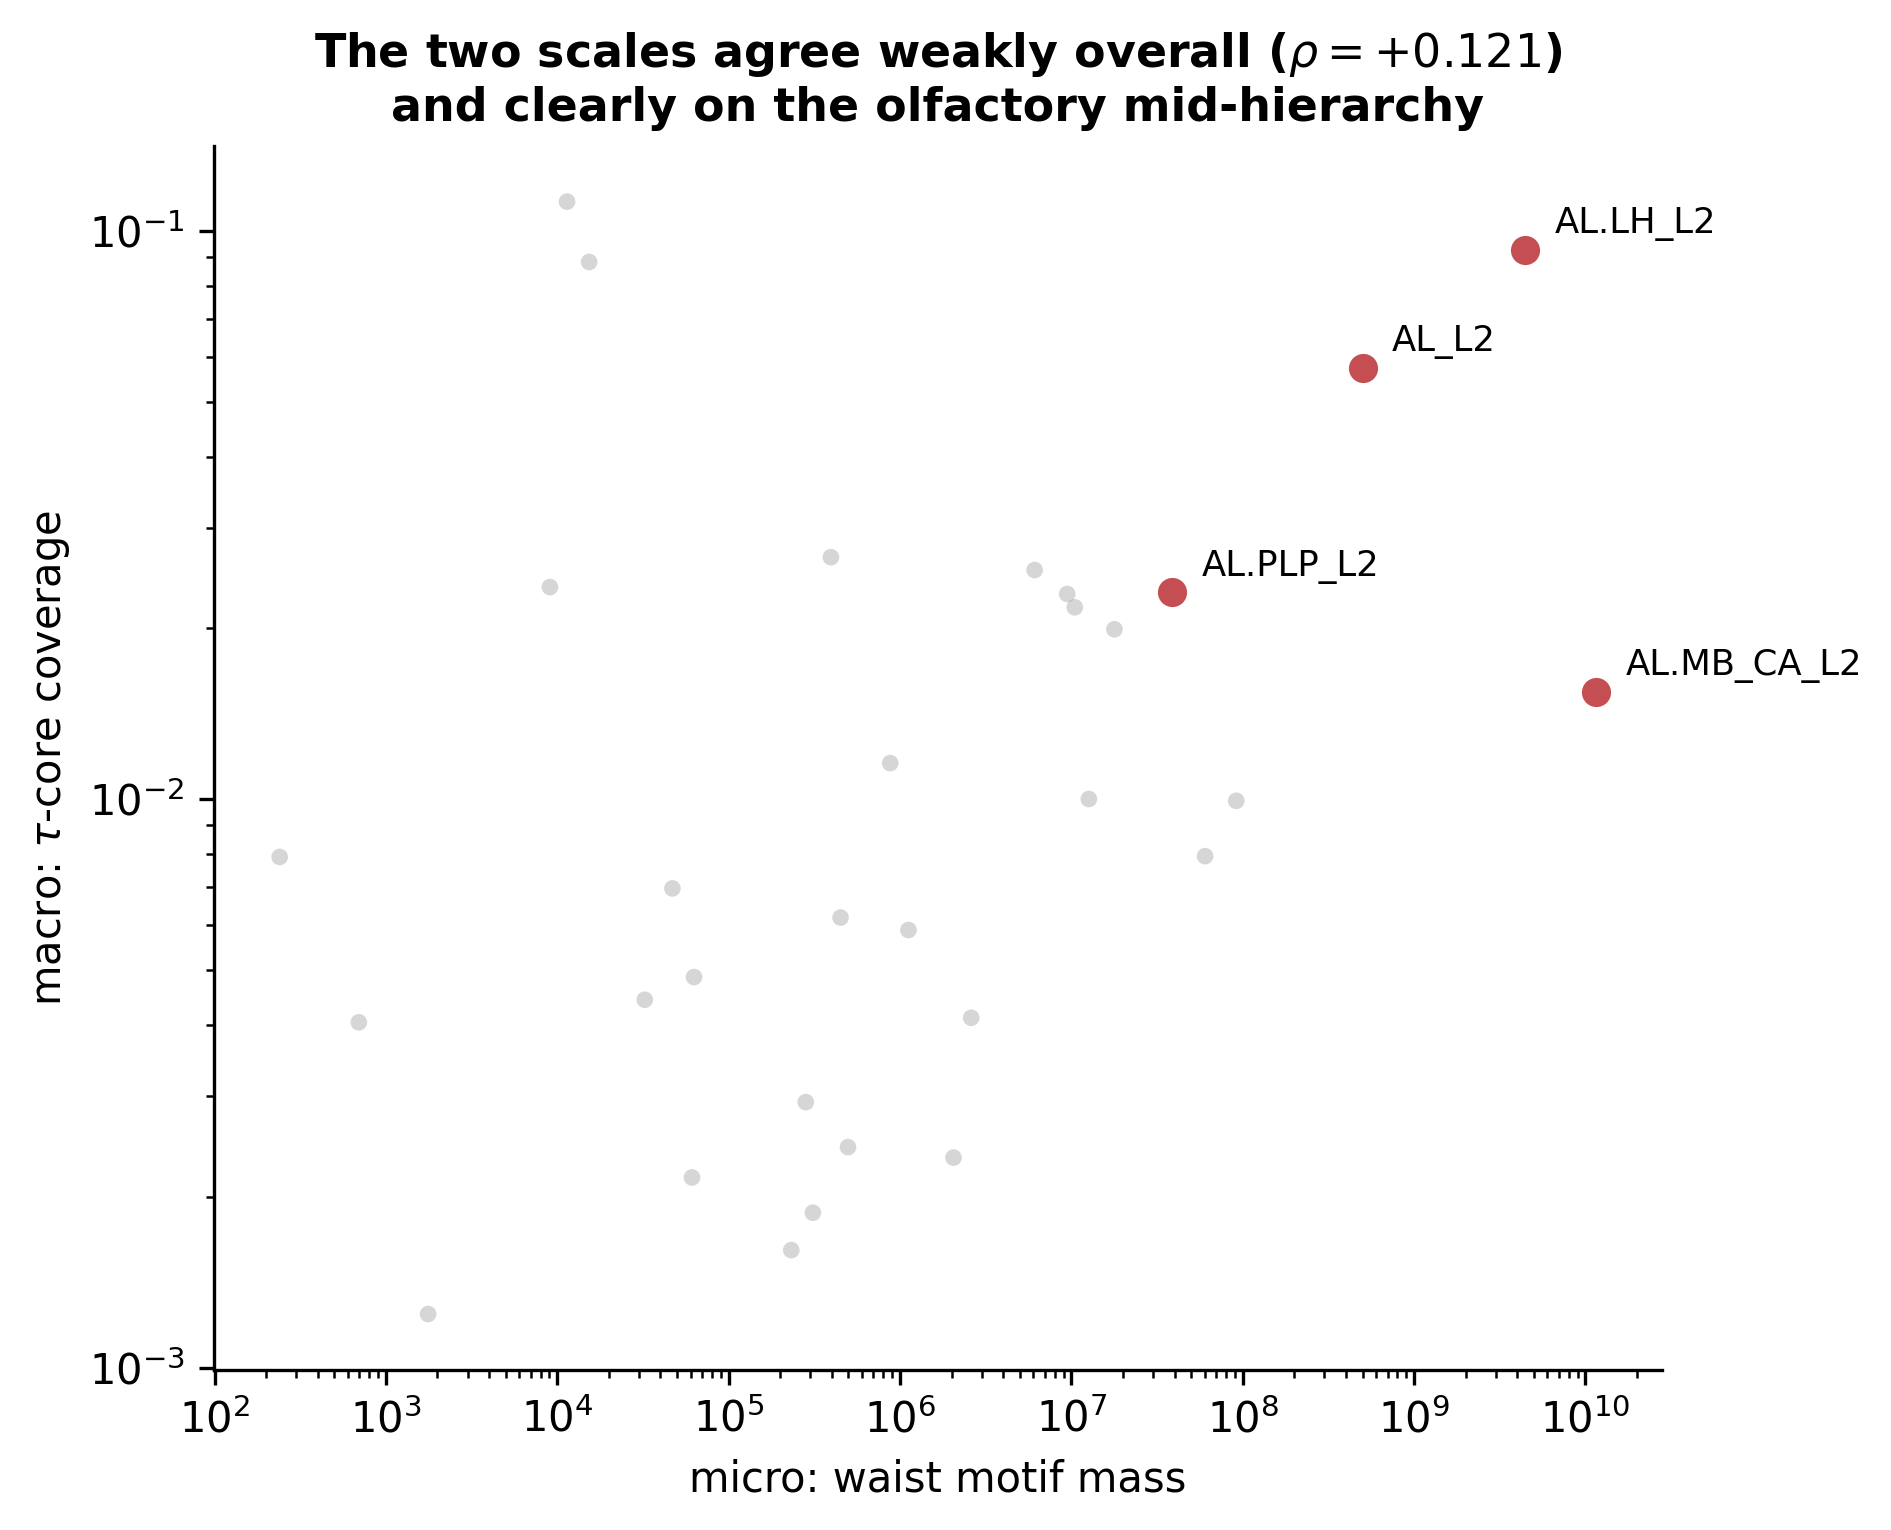
\includegraphics[width=0.72\textwidth]{micro_macro.png}
\caption[Agreement between the two scales]{Waist motif mass at the local
scale against $\tau$-core coverage at the global scale, one point per group
and level, with both axes logarithmic. The overall association is positive
but weak. Highlighted are the mid-hierarchy groups of the olfactory pathway,
on which the two scales agree closely.}
\label{fig:micro-macro}
\end{figure}

Where the two scales agree, they agree on the mid-hierarchy waists of the
olfactory pathway, as Table~\ref{tab:bridge} shows.

\begin{table}[H]
\centering
\caption{Groups where the two scales agree: mid-hierarchy waists of the
olfactory pathway, with ranks out of six hundred and sixty groups.}
\label{tab:bridge}
\begin{tabular}{lrr}
\toprule
Group & Micro rank (motif mass) & Macro rank (coverage) \\
\midrule
\code{AL.MB\_CA\_L2} &  8 & 12 \\
\code{AL.LH\_L2}     & 10 &  2 \\
\code{AL\_L2}        & 20 &  4 \\
\code{AL.PLP\_L2}    & 50 &  8 \\
\bottomrule
\end{tabular}
\end{table}

The overlap between the two top-twenty lists is three groups out of twenty.
Two lists of twenty drawn at random from six hundred and sixty would be
expected to share $0.61$ groups, a figure given by the hypergeometric
distribution, which describes how many elements two subsets of fixed size
share when drawn without replacement from the same population; observing
three gives $p = 0.0195$. That agreement is modest in absolute terms but is
concentrated on structures of known functional importance, which makes it
more meaningful than the raw number suggests.

The scales disagree on the input-side groups, and the disagreement is worth
examining rather than dismissing. Groups such as \code{GNG} and \code{PRW}
at level~1 are central in the global flow, appearing in the $\tau$-core,
while ranking very low as local waists. There is no contradiction here once
the two measurements are read carefully: being an obligatory passage point
on the way from sensation to action is a different property from being a
point at which many streams converge and then diverge locally. A relay
through which everything must pass will score highly on path centrality and
poorly on bow-tie counts, and the fly's early sensory structures are
precisely such relays.

On the deep window the global correlation is comparable, at $\rho = +0.103$
with $p = 0.001$, but the overlap of the top-twenty lists falls to one group
out of twenty and is no longer significant, with $p = 0.33$. This is the
expected outcome rather than a failure of replication, since the
$\tau$-core is dominated by olfactory and gustatory pathways which reside at
levels one to three and are therefore largely outside the deep window.

\subsection{Neurotransmitters: A Hypothesis and Its Scope}
\label{sec:results-nt}


The waists identified so far are structural objects, and a natural question
is whether they are also chemically distinct: whether the waists of backward
circuits, in particular, are more inhibitory than those of forward ones. The
hypothesis is plausible, since inhibition is commonly associated with
feedback control, and the data needed to test it are available, because
FlyWire predicts a neurotransmitter for every neuron, under the
classification set out in Section~\ref{sec:dataset}.

This section reports what came of it. Part of the answer is robust and is
stated first; the central comparison holds on one window and not on the
others, and the reason for the discrepancy is identified rather than left
open; and what survives is a narrower claim about one brain region, together
with the procedure that separated it from the broader one.

\subsubsection{What Holds}

Before turning to what does not hold, it is worth stating what does. The
composition of excitatory and inhibitory neurons by anatomical group is
robust across every window examined: \code{AL.MB\_CA} and the mushroom body
are essentially entirely excitatory, while the optic lobe and the lateral
horn are the most inhibitory structures in the brain. This result depends
only on counting neurons by their predicted neurotransmitter within each
group, and not on any comparison between classes of motif, which is why it
survives the difficulties described below.

Figure~\ref{fig:nt-direction} shows the related and also robust observation
that forward edges are more excitatory than backward ones. That difference,
however, is almost entirely attributable to the medulla, whose edges
dominate the forward class, and it is a statement about edges rather than
about waists.

\begin{figure}[H]
\centering

\includegraphics[width=0.86\textwidth]{nt_by_direction.png}
\caption[E/I composition by edge direction]{Excitatory and inhibitory
composition of edges by direction. Forward edges are more excitatory than
backward ones, but the difference is almost entirely attributable to the
medulla. This figure concerns edges; the waist-level comparison that
follows, which is the hypothesis actually under test, does not survive
replication.}
\label{fig:nt-direction}
\end{figure}

\subsubsection{What Does Not}

The hypothesis under test was that the waists of backward bow-ties differ
neurochemically from those of forward bow-ties. The natural way to test
it is to compare, for each waist group that hosts motifs of both kinds, the
excitatory fraction of that group as it appears in the two classes; working
at parity of waist in this way controls for the regional composition that
Section~\ref{sec:problem} identified as the principal confound.

Because each waist contributes one value to each class, the two samples are
paired rather than independent, and the comparison is made with the Wilcoxon
signed-rank test: the differences within each pair are ranked by magnitude
and the ranks of the positive and negative differences are compared. The
test is used rather than a paired $t$-test because the excitatory fractions
are proportions bounded in $[0,1]$ and far from normally distributed, with
many waists entirely excitatory or entirely inhibitory. Every $p$-value
reported in this section comes from that test.

On the shallow window the effect appears clear, with a gap of $+0.122$ at
$p = 0.0034$. Extending the same comparison to all four windows produces
Table~\ref{tab:nt} and Figure~\ref{fig:nt-windows}.

\begin{table}[H]
\centering
\caption{Excitatory fraction of the waist, \emph{pure\_BWD} against
\emph{pure\_FWD}, compared at parity of waist across all four level windows.}
\label{tab:nt}
\begin{tabular}{lrrrrr}
\toprule
Window & Shared waists & \emph{pure\_BWD} & \emph{pure\_FWD} & Gap at parity & $p$ \\
\midrule
$\{1,2,3\}$     &  86 & 0.387 & 0.508 & $+0.122$ & 0.0034 \\
$\{3,4,5\}$     & 221 & 0.501 & 0.547 & $+0.046$ & 0.0098 \\
$\{2,3,4\}$     & 185 & \textbf{0.506} & \textbf{0.449} & $\mathbf{-0.057}$ & 0.0296 \\
$\{1,2,3,4,5\}$ & \textbf{492} & 0.483 & 0.504 & $+0.021$ & \textbf{0.098} \\
\bottomrule
\end{tabular}
\end{table}

\begin{figure}[H]
\centering
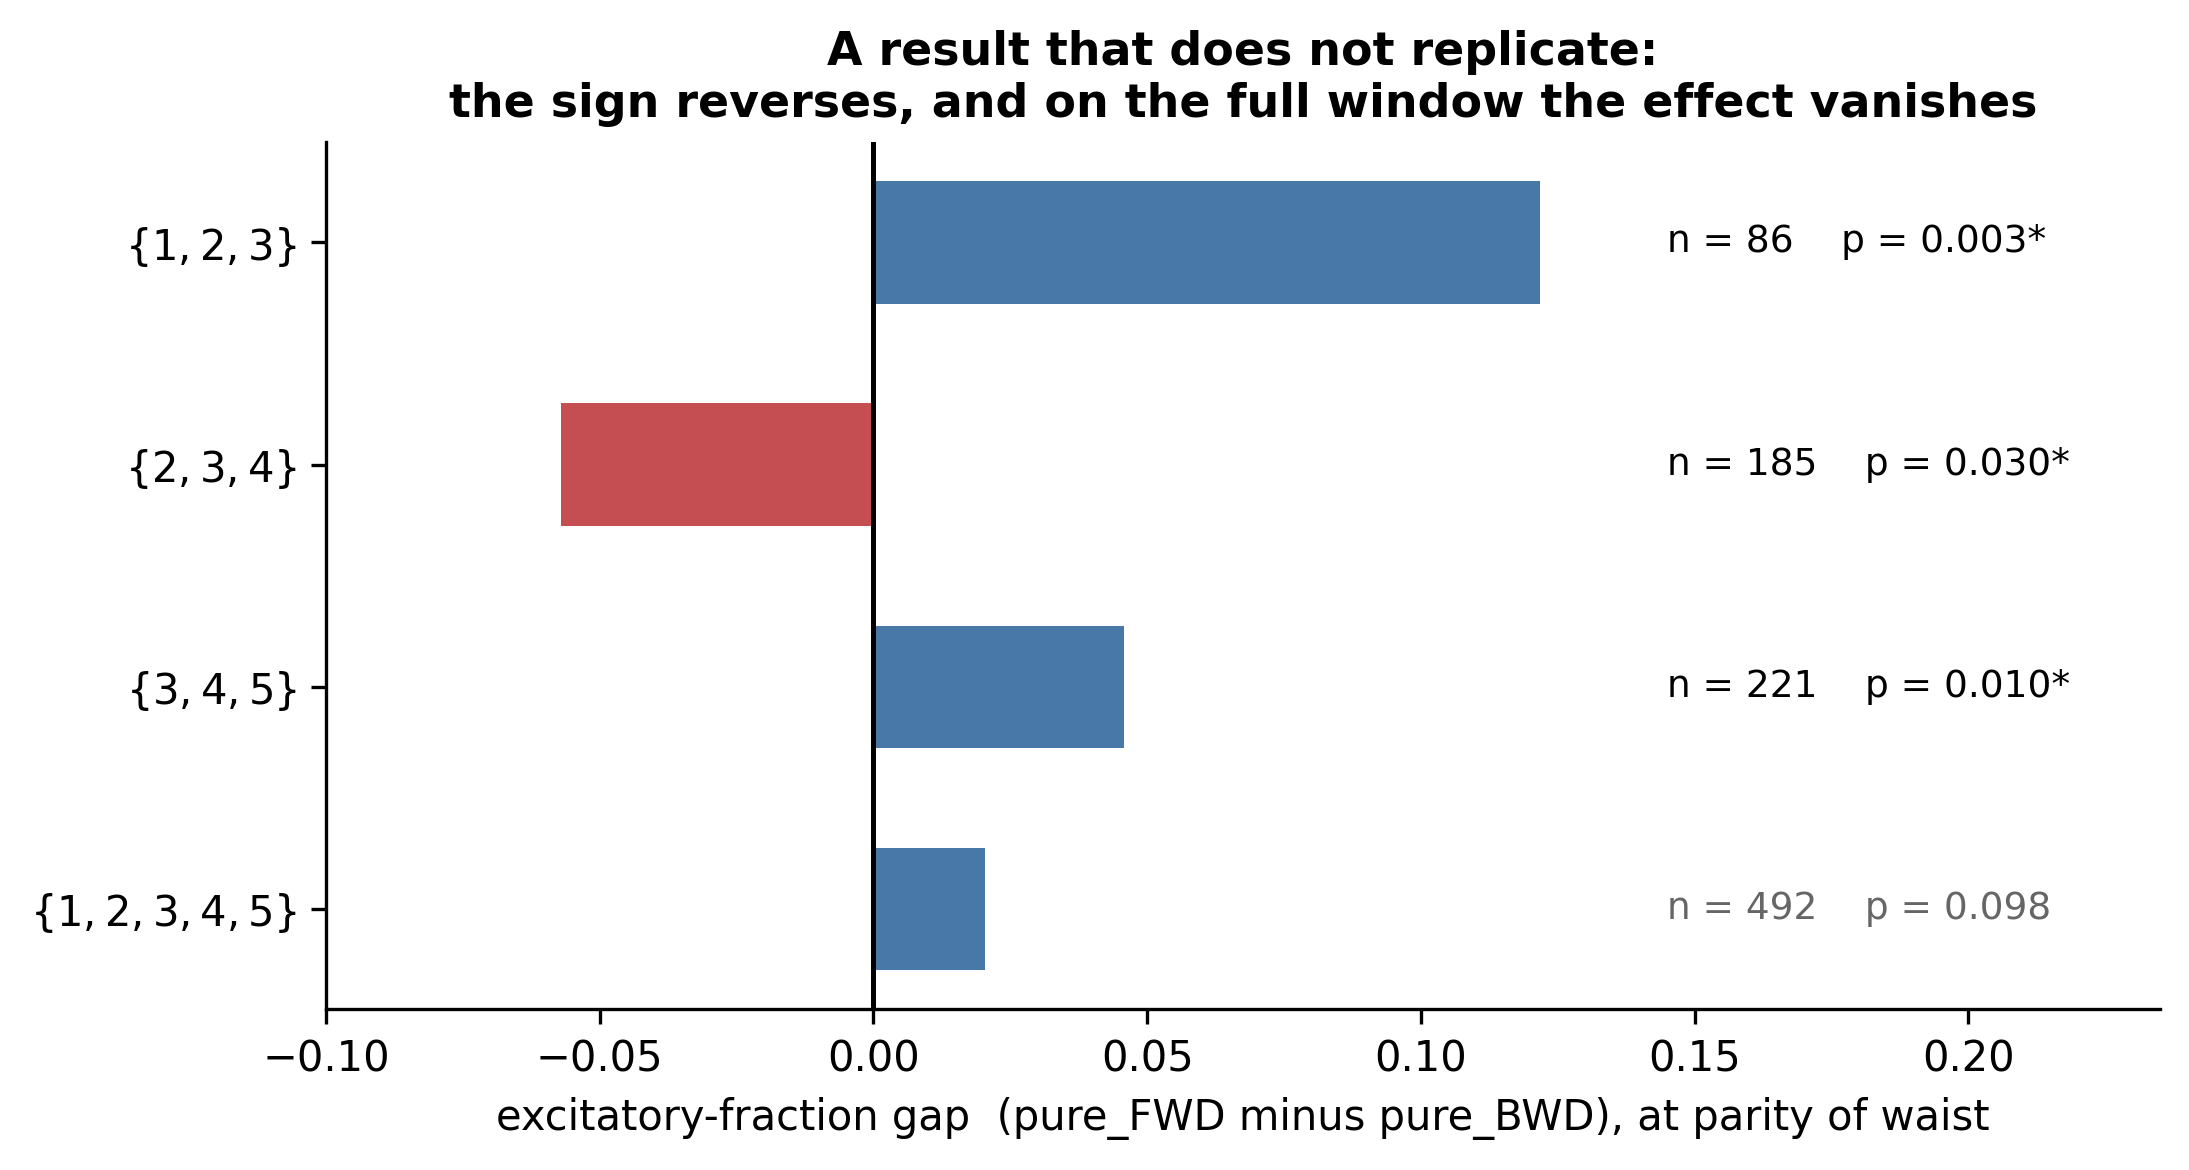
\includegraphics[width=0.90\textwidth]{nt_across_windows.png}
\caption[The neurotransmitter result across all four windows]{Excitatory
fraction gap between \emph{pure\_FWD} and \emph{pure\_BWD} waists, measured at
parity of waist, across all four level windows, with asterisks marking
$p < 0.05$. Window $\{2,3,4\}$ falls on the opposite side of zero from the
others, and the full window, which has the most shared waists and subsumes
the rest, does not reach significance.}
\label{fig:nt-windows}
\end{figure}

Three observations together dismantle the conclusion. On window
$\{2,3,4\}$ the sign of the effect reverses, with a $p$-value that would
conventionally be called significant: there, backward waists are
\emph{more} excitatory rather than less. On the full window, which has the
largest number of shared waists and which subsumes all the others, the
effect does not reach significance at all. And the raw gaps on those two
larger windows, before any control is applied, are essentially zero, at
$+0.0003$ and $+0.0021$ respectively, against $+0.726$ on the shallow
window; there is consequently not even an effect present to be explained.

\subsubsection{Why the First Window Looked Convincing}

The explanation lies in where the two classes of motif happen to sit. On the
shallow window the \emph{pure\_FWD} motifs concentrate in
\code{AL.MB\_CA}, which is essentially fully excitatory, while the
\emph{pure\_BWD} motifs concentrate in the optic lobe, which is inhibitory.
The apparent difference between motif classes is thus a difference between
brain regions wearing the costume of a difference between circuit types.

The control at parity of waist did substantial work: it removed $83\%$ of
the raw gap on that window, taking it from $+0.726$ down to $+0.122$. What
it did not do was remove all of it, and the residue looked like a genuine
effect. In hindsight the residue was the remaining part of the same
regional artefact, not an independent phenomenon, and the way this became
visible was replication rather than any refinement of the control itself.

It is also worth noting the multiple-testing situation. Across four windows
and six pairwise comparisons there are twenty-four tests in total, so
roughly one false positive is expected at a nominal $\alpha = 0.05$. None of
the four $p$-values in Table~\ref{tab:nt} survives a Bonferroni correction
within its own window, except the one obtained on the shallow window. The
Bonferroni correction is the most conservative way of accounting for
multiple tests: it divides the significance threshold by the number of tests
performed, so with six comparisons per window the level required drops from
$0.05$ to $0.0083$.

\subsubsection{What the Analysis Establishes}

Three things come out of this, and they should be kept apart.

The first is a claim that holds. Within the medulla, forward connections are
excitatory in $68.8\%$ of cases and backward ones in only $34.8\%$. This is
measured at parity of region, so it is not a composition effect, and it is
biologically unsurprising: the medulla contains the motion-detection
circuitry, in which lateral and feedback inhibition are the expected
mechanism. This is the version of the hypothesis that the data support.

The second is a claim that does not hold, at least not on this evidence: that
the same relation is a general property of the connectome. It is not
supported outside the optic lobe, and the analysis says why rather than
merely reporting that it failed. The two classes of motif are not spread
evenly across the brain, so a comparison between them is partly a comparison
between the regions they happen to occupy, and once that is controlled for
most of the effect is gone.

The third is a question left open. Whether some weaker version of the
relation holds in the central brain, where the two classes of motif are too
unevenly distributed for the present design to test it, is not settled here.
Answering it needs a different design rather than more data: a set of waists
selected in advance to carry both directions in comparable numbers, which
this analysis, working from an exhaustive search rather than a targeted one,
could not assemble. Section~\ref{sec:future} returns to this.

The procedure itself is the part that transfers. It has three steps:
control at parity of waist, decompose the raw gap to see how much of it the
control removes, and replicate across independent subsets of the data. The
last step was the decisive one, and its lesson is worth stating plainly. Two
concordant windows are not a replication but two draws from overlapping
data; it was only the third and fourth windows that made the scope of the
claim visible.

\subsection{Integrative, Broadcast and Mixed Networks}
\label{sec:results-sweep}

Everything so far has been counted with two inputs and two outputs, which
makes every pattern symmetric by construction. That symmetry is a
restriction on what can be seen, not a property of the connectome, and
lifting it turns out to reveal something the symmetric search cannot: not
just \emph{where} the bottlenecks are, but \emph{what kind of operation}
each one performs.

Allowing $\kin$ and $\kout$ to vary independently distinguishes three
regimes. A circuit with many inputs and one output is \emph{integrative}: it
gathers information from several sources and compresses it into one channel,
which is what a decision or a classification looks like structurally. A
circuit with one input and many outputs is a \emph{broadcast}: it takes one
signal and distributes it widely, which is what an expansion into a
higher-dimensional representation looks like. Balanced configurations are
mixed. The distinction is captured by an \emph{integration index}, negative
for broadcast and positive for integration, and the question this section
asks is whether the index, computed from wiring alone, recovers operations
that are known independently from physiology.

Enumeration is again avoided, this time by a different route. The sum over
all $k$-combinations of a product of flow vectors is the elementary
symmetric polynomial $e_k$ of those vectors, which can be evaluated in
$O(p \cdot k)$ time per neuron for $p$ available groups without ever forming
a single combination explicitly. The complete sweep for $k$ from two to five
on the shallow window takes ninety-four seconds, where explicit enumeration
would have required forming $2.9$ million combinations for a single waist at
$\kin = 3$.

One methodological caution applies to the resulting index, and it is
instructive because the artefact is easy to miss. The raw integration index
is confounded with the number of groups available to a waist, since $e_k$
over $p$ groups grows combinatorially with $p$: its Spearman correlation
with $\log(p/q)$, where $q$ is the number of output groups, is $+0.535$ at
$p = 3.6 \times 10^{-38}$. A waist with many neighbours would therefore
appear integrative purely on that account. Normalising by the number of
available combinations reduces the correlation to $-0.023$ at $p = 0.61$,
which eliminates the artefact, and only the normalised index is interpreted
here.

\subsubsection{The Sweep Recovers the Mushroom Body Architecture}

The window contains eight hundred and fifty-three metanodes, of which seven
hundred and five carry a total count of at least $10^3$ and are classified;
the rest are too sparsely populated for the index to mean anything. Of those
seven hundred and five, two hundred and forty-eight come out integrative,
three hundred and seventeen mixed and one hundred and forty broadcast. A tally of that kind
is not by itself informative: any classification of five hundred objects
into three bins will produce numbers, and nothing in them says whether the
bins mean anything.

What makes the classification testable is that there exists a circuit whose
answer is known in advance. The olfactory pathway of the mushroom body is
among the best characterised in any brain, and its computational
organisation has been established physiologically rather than structurally:
a compact odour code carried by a few dozen projection neuron types is
expanded onto a much larger population of Kenyon cells, and that expanded
representation is then read out by a small number of output neurons whose
activity drives behaviour. Expansion followed by compression is exactly the
sequence broadcast $\rightarrow$ mixed $\rightarrow$ integrative would
describe, so the pathway constitutes a prediction the index either meets or
fails.

Table~\ref{tab:mb-architecture} therefore reports the five metanodes lying
along that pathway rather than the highest-scoring metanodes overall. The
selection is made anatomically and before looking at the index: they are the
waists corresponding to the antennal-lobe projection neurons, to the
parallel projection into the lateral horn, to the Kenyon cells, and to the
two mushroom body output populations. Reporting the extremes of the ranking
instead would have shown only that the index has extremes.

\begin{table}[H]
\centering
\caption{Normalised integration index along the olfactory pathway. Negative
values indicate broadcast, positive values integration.}
\label{tab:mb-architecture}
\begin{tabular}{lrrl}
\toprule
Waist & in / out & Index & Regime \\
\midrule
\code{AL.MB\_CA\_L2} (projection neurons) & 46 / 99 & $-0.895$ & broadcast \\
\code{AL.LH\_L2}                          & 100 / 192 & $-0.712$ & broadcast \\
\code{MB\_CA.MB\_ML\_L3} (Kenyon cells)   & 58 / 53 & $+0.061$ & mixed \\
\code{MB\_ML.CRE\_L2} (MB output)         & 45 / 47 & $+0.997$ & integrative \\
\code{MB\_PED.CRE\_L2}                    & 28 / 29 & $+1.000$ & integrative \\
\bottomrule
\end{tabular}
\end{table}

\begin{figure}[H]
\centering
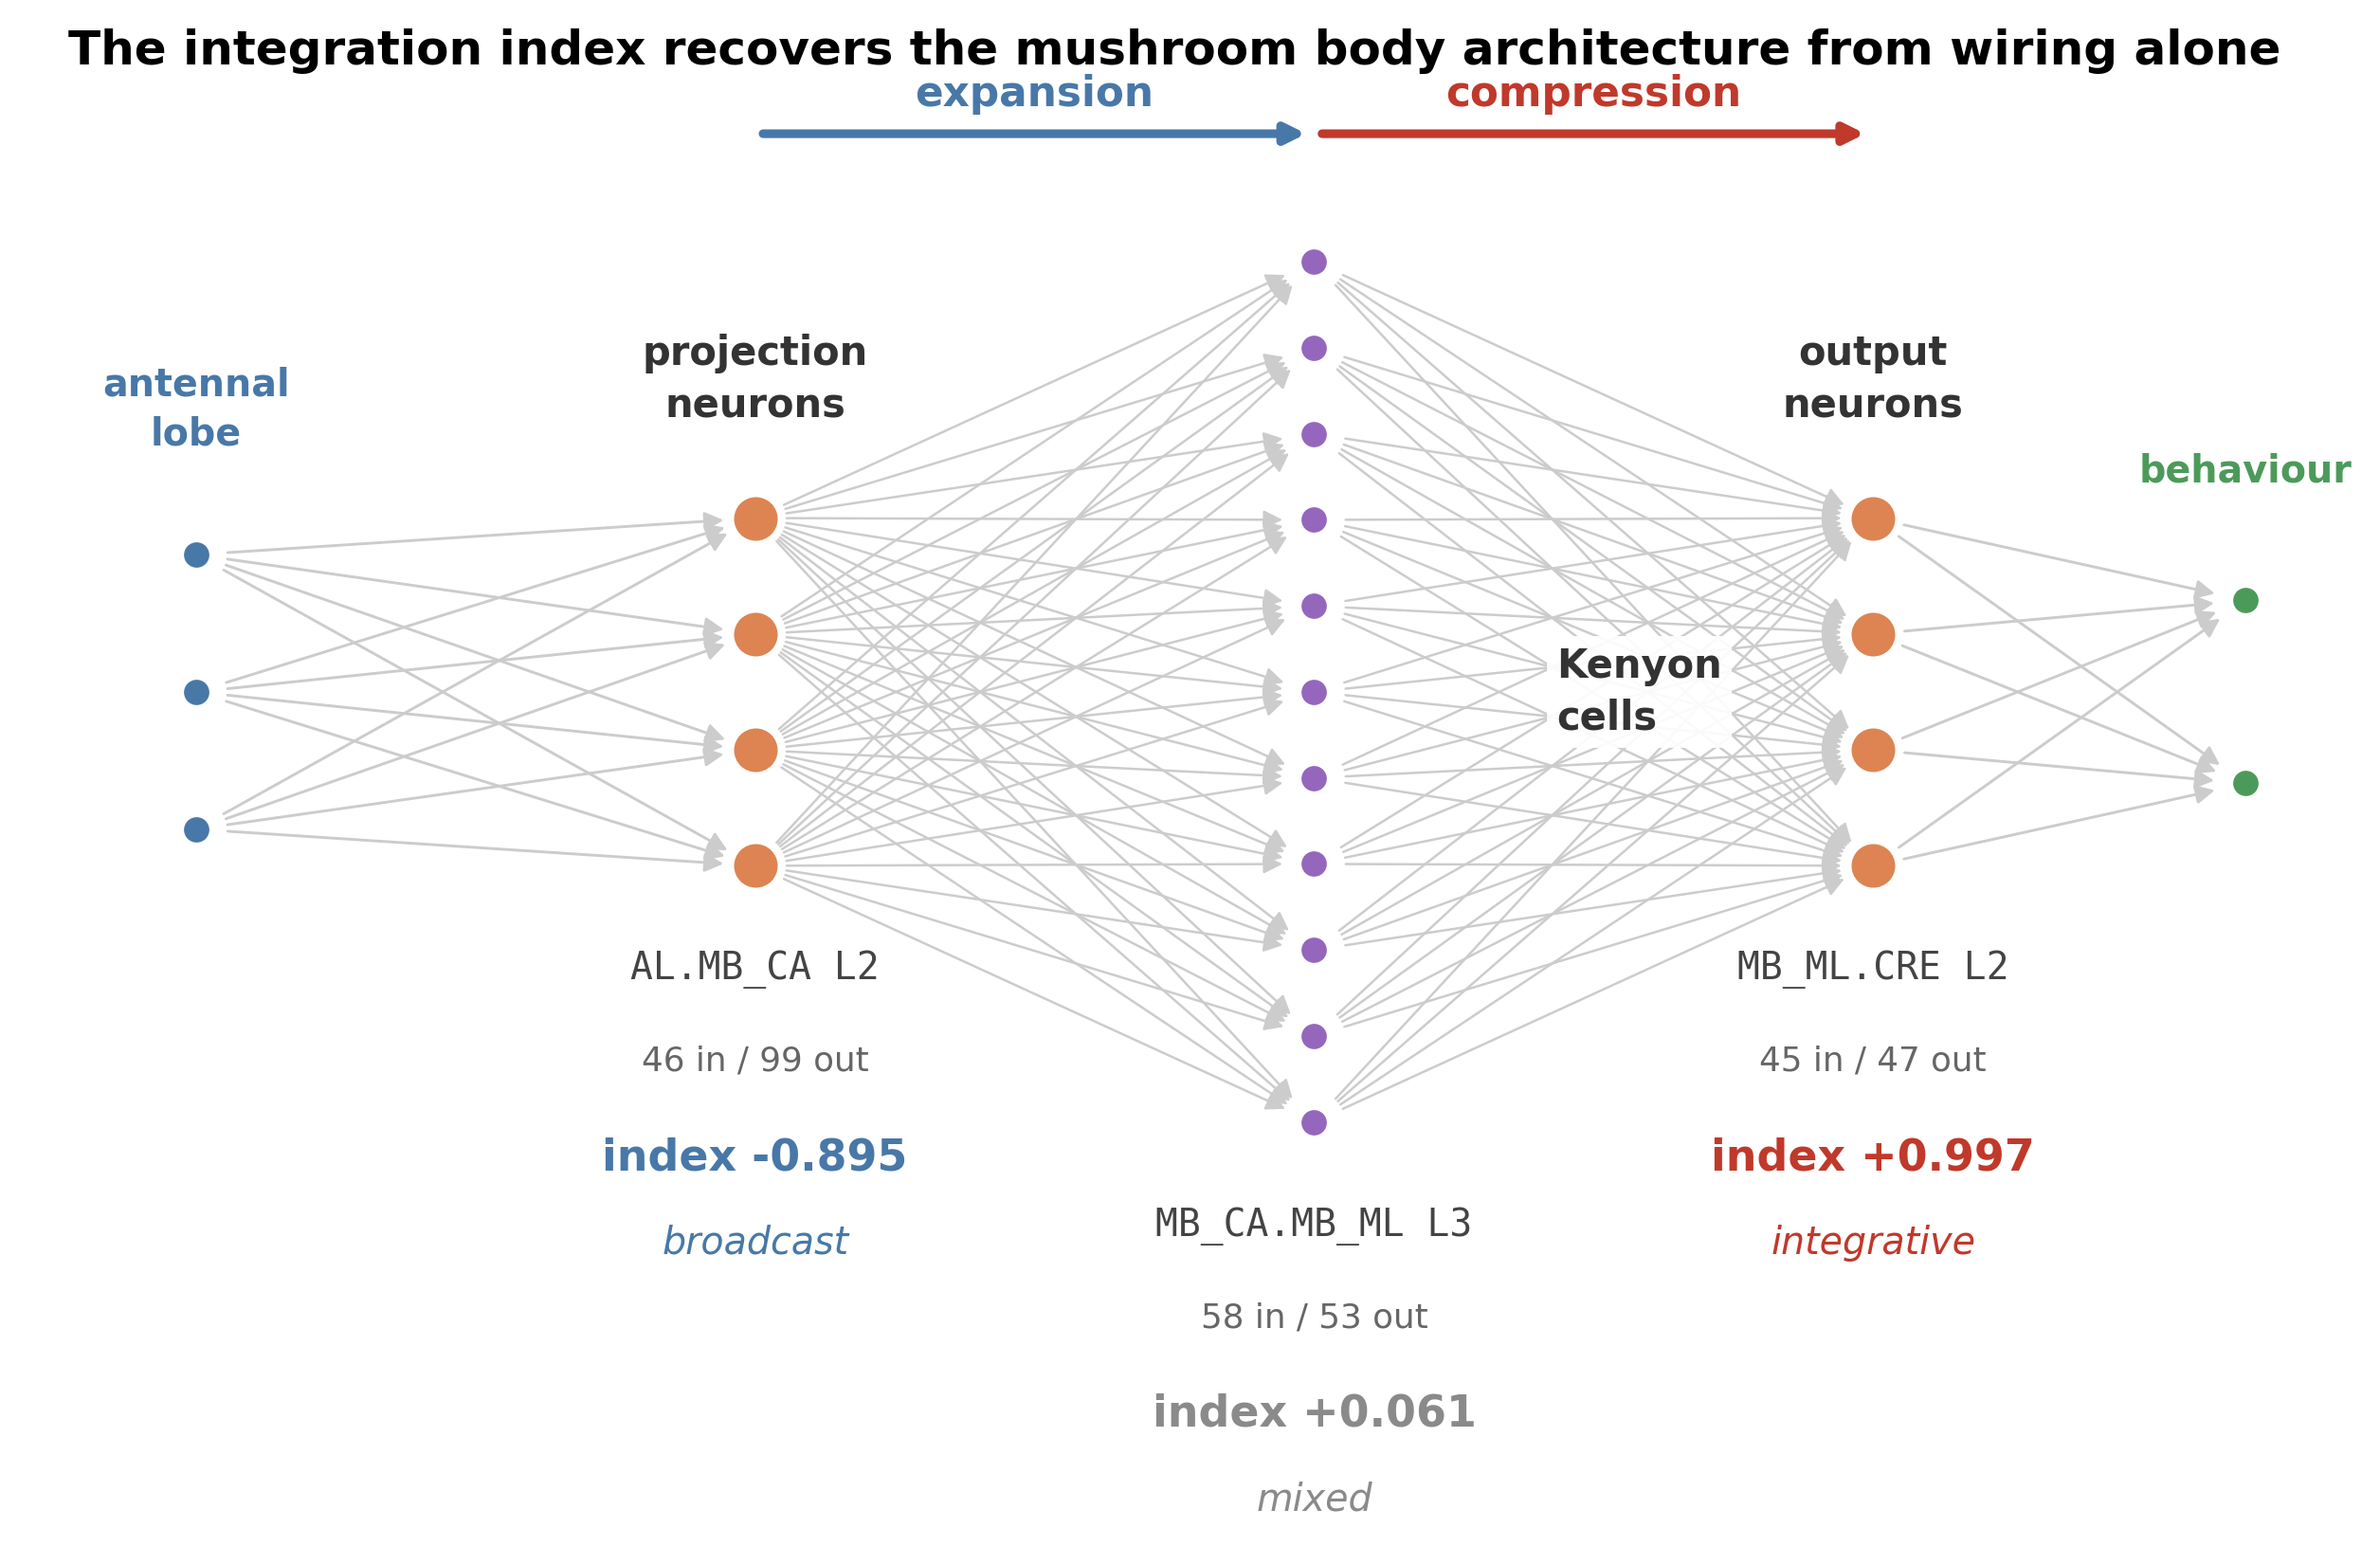
\includegraphics[width=\textwidth]{olfactory_pathway.png}
\caption[The olfactory pathway recovered by the integration index]{The
olfactory pathway of the mushroom body, drawn so that the width of each
stage reflects the operation the index attributes to it. Odour information
arrives from the antennal lobe, is distributed by a small population of
projection neurons onto a much larger one of Kenyon cells, and is then read
out by a small population of output neurons. The integration index beneath
each stage is computed from connectivity alone, with no anatomical
information supplied: it comes out strongly negative where the circuit
expands, near zero where it is maintained, and at the extreme of positive
where it compresses. The values are those of
Table~\ref{tab:mb-architecture}.}
\label{fig:olfactory}
\end{figure}

The prediction is met, and in order, as Figure~\ref{fig:olfactory} shows.
The two entries at the top of the
table, the projection neurons and the parallel pathway into the lateral
horn, come out strongly negative at $-0.895$ and $-0.712$: they are
broadcasts, distributing a compact odour representation outwards. The Kenyon
cells sit almost exactly at the boundary, $+0.061$, which is the mixed
regime: they receive the expansion and pass it on without yet compressing
it. The two output populations come out at $+0.997$ and $+1.000$, at the
extreme of integration: they collapse the expanded representation back into
a few channels. Read down the table, the index traces expansion, then
maintenance, then compression, which is the textbook description of the
circuit.

Three things follow, and they are worth separating because they are claims
of different strength.

The first concerns the index rather than the biology. The ordering was
recovered from connectivity alone, with no anatomical or physiological
information supplied at any stage, and with the selection of rows fixed in
advance. That is what makes it a test: the index could have come out flat,
or in the wrong order, and it did not. This is the strongest of the three
statements and it is a validation of the method.

The second concerns what the index adds to the rest of the thesis. The
symmetric search of Section~\ref{sec:results-windows} identifies
\code{MB\_CA.MB\_ML} and the mushroom body waists as high-count structures,
but it describes them all the same way, since with $\kin = \kout = 2$ every
pattern is symmetric by construction. The sweep separates them: the
projection neurons and the output neurons are both bottlenecks, and both
carry a great deal of mass, and yet they are performing opposite operations.
The direction of the asymmetry is information the fixed-shape search
discards, and recovering it costs ninety-four seconds.

The third is a caution about scope. The mushroom body is the case where the
answer was known, which is precisely why it was used, and a method validated
on one circuit has not thereby been validated on all of them. The remaining
seven hundred metanodes carry index values too, and nothing here establishes
that those values are equally meaningful. What the mushroom
body licenses is the weaker and still useful claim that the index is capable
of recovering a real computational organisation when one is present, which
makes it worth applying elsewhere and worth checking against physiology
wherever such a check is available.

\subsection{Within-Area Characterisation}
\label{sec:results-within}

The analyses so far have studied interactions \emph{between} anatomical
areas. A complementary question is what the motif composition looks like
\emph{within} a single area, and whether areas differ from one another in
that respect.

An area here is a neuropil, and a neuron is taken to belong to every
neuropil named in its group assignment, so that a neuron labelled
\code{AL.MB\_CA} counts towards both the antennal lobe and the mushroom body
calyx. Areas therefore overlap, which is anatomically correct: a projection
neuron genuinely does arborise in both structures. Of the forty-four
neuropils in the dataset, thirty-five contain at least two hundred neurons
and are analysed here.

Counting within a single area raises a difficulty that does not arise
between areas. Reciprocal connections within one neuropil are frequent, so
the sets of neurons available as inputs and as outputs overlap heavily, and
the requirement that the five participating neurons be distinct can no
longer be handled by simply choosing disjoint groups. The count is therefore
computed in closed form with an inclusion--exclusion correction that
subtracts the configurations in which neurons coincide. Explicit enumeration
would be quite infeasible, requiring on the order of $10^{10}$ combinations
in the medulla alone, whereas the closed form processes the entire
connectome in $4.5$ seconds. The formula was verified against exhaustive
enumeration on three hundred random graphs, with exact agreement on all
sixteen signatures.

\subsubsection{What Survives the Null, and What the Null Removes}

Across five hundred and sixty tests, being thirty-five areas by sixteen
signatures, one hundred and one are significant at $q < 0.05$ after
Benjamini--Hochberg correction. The comparison worth reporting, however, is
not that count but what changes between the naive analysis and the
controlled one.

\begin{table}[H]
\centering
\caption{Enrichment before and after applying the within-area null model.
The naive comparison against the global profile produces large values that
the null removes entirely.}
\label{tab:within-null}
\begin{tabular}{lrrr}
\toprule
Area & Naive enrichment & Versus null & $q$ \\
\midrule
\code{EB} & $12.6\times$ & $\mathbf{1.00\times}$ & $1.00$ \\
\code{MB\_CA} & --- & $0.76\times$ & $1.00$ \\
\code{NO} & $13.5\times$ & $1.99\times$ & $0.028$ \\
\code{FB} & $7.3\times$  & $1.84\times$ & $0.028$ \\
\bottomrule
\end{tabular}
\end{table}

The ellipsoid body falls from an apparent twelve-fold enrichment to exactly
one-fold: the entire effect was a consequence of how that area's neurons are
distributed across levels, and the null neutralises it completely. The
noduli and the fan-shaped body retain a smaller but genuine enrichment of
roughly twice the null expectation. The null model therefore does both of
the jobs asked of it, removing false positives while preserving real
signals, which is the property that makes the surviving results worth
reporting.

Three findings survive the control. The antennal lobe shows $31\%$ of its
motifs in the \code{LAT->LAT} class, with its neurons spread across several
levels rather than concentrated in one, and it is the only genuinely
informative lateral case in the dataset. It corresponds to the network of
local interneurons that performs lateral inhibition between olfactory
glomeruli, the spherical compartments of the antennal lobe in which the
receptors for a single odorant type converge, which is a well-established circuit recovered here independently
and not explicable by level concentration. The optic lobe shows the
re-entrant medulla pattern at $57.3\%$ and the lobula plate relay at
$40.9\%$, consistent with Section~\ref{sec:optic-recurrence} and reached by
an entirely independent route. The associative areas, by contrast, show no
comparable structure, which is itself informative: the lateral organisation
observed elsewhere is specific to particular circuits rather than a generic
property of dense tissue.

\subsection{Computational Performance}
\label{sec:results-performance}

Table~\ref{tab:performance} reports the effect of the sparse reformulation
on the two most expensive waists of the search.

\begin{table}[H]
\centering
\caption{Effect of the sparse reformulation on the most expensive
bottlenecks.}
\label{tab:performance}
\begin{tabular}{lrrr}
\toprule
Bottleneck & Before & After & Speed-up \\
\midrule
\code{ME\_L2} ($|B| = 24{,}835$) & 3172\,s & 14.5\,s & $219\times$ \\
\code{ME\_L3} ($|B| = 10{,}709$) & 355\,s  & 1.4\,s  & $254\times$ \\
\bottomrule
\end{tabular}
\end{table}

The single waist \code{ME\_L2} previously accounted for roughly half of the
total runtime on the shallow window, which is what makes a change of this
magnitude on one bottleneck worth the effort. With the sparse engine in
place, no waist falls back to the reference loop on any of the deeper
windows. End to end, the shallow window went from one hour and forty-four
minutes to fourteen minutes and thirty-nine seconds.

Output distillation, described in Section~\ref{sec:distillation}, reduced
the four windows from over $100$\,GB to $68$\,MB, a reduction of up to
$18{,}847$-fold on the largest window, while producing downstream results
that are identical to those obtained from the full output. The distillation
itself costs approximately thirty per cent of the search time, since the
aggregates must be maintained as the rows are produced; this is the price of
not writing the intermediate at all, and it is worth paying only because the
search has become fast enough that regenerating the rows costs less than
storing them.

%=======================================================================
\section{Conclusions}
\label{sec:conclusions}
%=======================================================================

\subsection{Summary of Contributions}

This thesis analysed the bow-tie architecture of the adult \Dros{}
connectome at two complementary scales, and its contributions fall into four
groups.

The theoretical contribution is the characterisation of when motif counts
compose, stated as Proposition~\ref{prop:algebra}. The boundary between
linear counting and the \sigmapi{} formulation is the presence of branching,
and cyclic patterns require quadratic memory and are therefore out of reach
at connectome scale. The result is verifiable by exhaustive enumeration, was
so verified on all thirty-one patterns up to four nodes, and applies beyond
this particular connectome to any counting problem of the same shape. The
accompanying catalogue also places the method honestly: already at four
nodes, $87\%$ of connected patterns fall outside what it can handle.

The computational contribution is to have made exhaustive counting
tractable. Reformulating the inner loop as a matrix product delegated to
optimised libraries, and then switching to a sparse product on the large
waists where the dense form fails, produced a factor of $219$ on the worst
bottleneck and reduced the shallow window from one hour and forty-four
minutes to under fifteen. Recognising that the row-level output is an
intermediate rather than a result reduced storage from over $100$\,GB to
$68$\,MB with no loss to any analysis.

The empirical contributions concern the architecture itself. The hourglass
property is present, with a score of $0.498$ under structural routing, but
it depends on the routing scheme and is markedly weaker than in
\textit{C.\ elegans}, plausibly because the fly maintains several parallel
modality-specific bottlenecks rather than one shared one. The deep brain is
laterally dominated, with purely lateral branches carrying $82.6\%$ of the
motif mass against $38.0\%$ in the shallow brain. The deepest level of the
hierarchy is the most internally dense and yet marginal as a waist, a
combination that points to recurrent rather than convergent organisation.
And the two scales of analysis agree on the mid-hierarchy olfactory waists
while diverging interpretably on input groups.

The methodological contribution is the way an initially broad hypothesis was
narrowed to the claim the data actually support. An apparent neurochemical
difference between backward and forward waists held on the shallow window,
did not replicate on the others, and was traced to the regions the two
classes of motif occupy; what remains is a specific and defensible statement
about the medulla, and an open question about the central brain that needs a
targeted design to answer. The related finding that the ranking between
signatures inverts between null models makes the same point from a different
direction: single-null analyses of this kind can be confidently wrong.

\subsection{Limitations}

The hierarchical decomposition on which everything else rests is inherited
from earlier work rather than derived here, and it is only partly tested.
The functional gradient of Section~\ref{sec:results-hierarchy} supports the
spectral embedding that produces the underlying axis, but it cannot validate
the four thresholds placed on that axis, because those thresholds were
themselves chosen to separate the super-classes whose gradient is then
observed. Section~\ref{sec:results-coherence} establishes that the levels
are at least as compatible with the anatomical grouping used here as with
the one they were built for, which addresses a different concern. Where the
boundaries fall therefore remains an untested inheritance, and any result
conditioned on levels carries whatever assumptions went into producing
them.

The hourglass score depends on the routing scheme, taking values between
$0.247$ and $0.498$ depending on the scheme and the path-length bound. No
single number should be quoted in isolation, and the comparison with
\textit{C.\ elegans} should be read with the same caution, since the two
studies do not use identical routing conventions.

The coarse motif classification is close to vacuous, with $94.4\%$ of
patterns falling into the \emph{mixed} bucket. The sixteen-signature
decomposition addresses this, but even after it the residual
\code{mix->mix} class retains $29.5\%$ of patterns in the shallow window.
Resolving that class further would require distinguishing branches by which
specific levels they connect, at the cost of a considerably larger label
space.

No null model isolates the hypothesis cleanly. The three used here preserve
different constraint sets and none is fully satisfactory: model A preserves
global degrees but destroys anatomy, model B preserves anatomy but destroys
degrees, and model C preserves both while having a ratio dominated by
sparsity. A null that simultaneously preserved within-block degrees and
block densities would make the statistic essentially deterministic, since
the motif count is very nearly a deterministic function of the degree
sequences. The limitation is intrinsic to the quantity being tested rather
than to the implementation, and Section~\ref{sec:null-inversion} shows that
it has real consequences for interpretation.

Realised compression remains sensitive to a collapsing waist. When the flow
is carried by a single neuron the ratio explodes, with \code{LO\_L3}
reaching $6316$ at an effective waist of $1.3$ and \code{ME\_L2} reaching
$4259$ at $1.8$. Such structures are hubs rather than waists and are
excluded here by a threshold on the effective waist size, set to five
throughout, but that threshold is a declared choice and results should be
checked for robustness against it. Reporting the pair consisting of the
effective size and the periphery, instead of their ratio, would avoid the
division entirely and is worth considering.

The pattern catalogue stops at four nodes, since exhaustive enumeration on
five would require $2^{20}$ edge masks over $120$ permutations. The
classification of Proposition~\ref{prop:algebra} does not depend on pattern
size, so the qualitative conclusion carries, but the proportion of
non-factorisable patterns beyond four nodes is not measured here. Relatedly,
that proposition concerns homomorphisms, whereas the requirement that
participating neurons be distinct is a separate inclusion--exclusion layer;
the two should be kept conceptually apart.

The sweep over $\kin$ and $\kout$ covers only the pure forms, because the
symmetric-polynomial shortcut it relies on admits an exact disjointness
correction only for those. This is a limitation of the sweep and not of the
search engine, which counts any configuration exactly; what limits the engine
at larger $\kin$ and $\kout$ is the combinatorial growth of the number of
group combinations, not correctness.

The distillation fixes the selection criteria at search time, since the
retained top-$N$ selections are chosen by occurrence count. An analysis
requiring a different criterion, such as selection by realised compression,
would require re-running the search rather than merely re-reading the
stored output.

Finally, and most fundamentally, all the results here are structural.
Connectivity constrains computation but does not determine it, and no claim
about neural dynamics follows directly from these counts. What a structural
analysis can establish is which circuits exist and in what abundance; what
they do remains a question for physiology.

\subsection{Future Directions}
\label{sec:future}

The most immediate extension is to carry the remaining analyses through to
the deep windows. Realised compression and statistical validation were
conducted in depth only on the shallow window, which is the least rich of
the four with thirty-one million motifs against four hundred and thirty-four
million, and there is no methodological obstacle to repeating them now that
the search is fast enough.

The open question left by Section~\ref{sec:results-nt} calls for a targeted
design rather than more data. Testing whether backward waists are more
inhibitory than forward ones in the central brain requires a set of waists
chosen in advance to carry both directions in comparable numbers, since the
present comparison is confounded by the regions the two classes of motif
happen to occupy. An exhaustive search cannot assemble such a set, because it
takes the waists the connectome provides; a targeted search over waists
pre-selected for balance could, and would settle whether the medulla result
generalises or is specific to motion-detection circuitry.

The behaviour of level~5 deserves separate investigation. It is the most
internally dense level of the connectome and yet marginal as a waist, and
characterising the connectivity that produces this combination, presumably
recurrent and lateral rather than convergent, is a well-posed structural
question with a plausible functional interpretation attached to it.

The framework already supports arbitrary values of $\kin$ and $\kout$, so a
systematic exploration of asymmetric configurations would connect the
bow-tie analysis to the integrative and broadcast distinction of
Section~\ref{sec:results-sweep} in a more thorough way than the present
sweep allows.

Finally, both the counting framework and the hourglass measurement are
species-agnostic. Applying them to other fully mapped connectomes as those
become available would establish whether the architectural principles found
here are general or particular to the fly, which is the question that
motivates structural connectomics in the first place.


\begin{thebibliography}{99}
\addcontentsline{toc}{section}{Bibliography}

\bibitem{bassett2017}
D.~S. Bassett and O.~Sporns.
\newblock Network neuroscience.
\newblock \emph{Nature Neuroscience}, 20(3):353--364, 2017.

\bibitem{benjamini1995}
Y.~Benjamini and Y.~Hochberg.
\newblock Controlling the false discovery rate: a practical and powerful
  approach to multiple testing.
\newblock \emph{Journal of the Royal Statistical Society, Series B},
  57(1):289--300, 1995.

\bibitem{bullmore2009}
E.~Bullmore and O.~Sporns.
\newblock Complex brain networks: graph theoretical analysis of structural and
  functional systems.
\newblock \emph{Nature Reviews Neuroscience}, 10(3):186--198, 2009.

\bibitem{cordella2004}
L.~P. Cordella, P.~Foggia, C.~Sansone, and M.~Vento.
\newblock A (sub)graph isomorphism algorithm for matching large graphs.
\newblock \emph{IEEE Transactions on Pattern Analysis and Machine
  Intelligence}, 26(10):1367--1372, 2004.

\bibitem{corradini2025}
E.~Corradini, F.~Parlapiano, A.~Ronci, G.~Terracina, and D.~Ursino.
\newblock A complex network-based approach to detect and investigate
  connectome motifs in the larval \emph{Drosophila}.
\newblock \emph{Computers in Biology and Medicine}, 192, 2025.

\bibitem{curcio2026}
D.~Curcio.
\newblock \emph{Decoding the Drosophila Brain: A Parametric Framework for
  Hierarchical Motif Discovery in the Adult Connectome}.
\newblock Master's thesis, University of Applied Sciences Upper Austria and
  University of Calabria, 2026.

\bibitem{ito2014}
K.~Ito et al.
\newblock A systematic nomenclature for the insect brain.
\newblock \emph{Neuron}, 81(4):755--765, 2014.

\bibitem{lin2024}
A.~Lin et al.
\newblock Network statistics of the whole-brain connectome of
  \emph{Drosophila}.
\newblock \emph{Nature}, 634(8032):153--165, 2024.

\bibitem{maslov2002}
S.~Maslov and K.~Sneppen.
\newblock Specificity and stability in topology of protein networks.
\newblock \emph{Science}, 296(5569):910--913, 2002.

\bibitem{milo2002}
R.~Milo, S.~Shen-Orr, S.~Itzkovitz, N.~Kashtan, D.~Chklovskii, and U.~Alon.
\newblock Network motifs: simple building blocks of complex networks.
\newblock \emph{Science}, 298(5594):824--827, 2002.

\bibitem{sabrin2020}
K.~M. Sabrin, Y.~Wei, M.~P. van~den Heuvel, and C.~Dovrolis.
\newblock The hourglass organization of the \emph{Caenorhabditis elegans}
  connectome.
\newblock \emph{PLOS Computational Biology}, 16(2):e1007526, 2020.

\bibitem{tricoli2025}
M.~Tricoli.
\newblock \emph{Structural Modeling of the Drosophila melanogaster Connectome:
  Motif-Based and Hierarchical Analysis}.
\newblock Master's thesis, University of Calabria, 2025.

\bibitem{ullmann1976}
J.~R. Ullmann.
\newblock An algorithm for subgraph isomorphism.
\newblock \emph{Journal of the ACM}, 23(1):31--42, 1976.

\bibitem{winding2023}
M.~Winding et al.
\newblock The connectome of an insect brain.
\newblock \emph{Science}, 379(6636):eadd9330, 2023.

\end{thebibliography}

\end{document}
